\documentclass[11pt,reqno]{amsart}
\usepackage{iftex}
\ifPDFTeX
  \usepackage[T1]{fontenc}
  \usepackage[utf8]{inputenc}
  \usepackage{lmodern}
\else
  \usepackage[no-math]{fontspec}
\fi
\usepackage{amsmath}
\usepackage{amssymb}
\usepackage{amsfonts}
\usepackage{mathrsfs}
\usepackage{amsthm}
\usepackage{mathtools}
\usepackage{geometry}
\usepackage{enumitem}
\usepackage{longtable}
\usepackage{booktabs}
\usepackage{array}
\usepackage{microtype}
\usepackage{graphicx}
\graphicspath{{../figures/}{figures/}}
\usepackage[dvipsnames]{xcolor}
\usepackage{float}
\usepackage{listings}
\lstset{basicstyle=\ttfamily\scriptsize,breaklines=true,columns=fullflexible,keepspaces=true,
  frame=single,framerule=0.3pt,showstringspaces=false,keywordstyle=\color{NavyBlue},
  commentstyle=\color{OliveGreen},stringstyle=\color{BrickRed},upquote=true}
\usepackage[pagebackref=true]{hyperref}
\usepackage{bookmark}
\usepackage{pdfcomment}

% Hover previews for internal references (no layout change).
\makeatletter
\let\CG@origref\ref
\let\CG@origeqref\eqref
\newcommand{\CG@gettip}[1]{\@ifundefined{CGTip@#1}{Reference: #1}{\csname CGTip@#1\endcsname}}
\DeclareRobustCommand{\CGref}[1]{\pdftooltip{\CG@origref{#1}}{\CG@gettip{#1}}}
\DeclareRobustCommand{\CGeqref}[1]{\pdftooltip{\CG@origeqref{#1}}{\CG@gettip{#1}}}
\makeatother
% Tooltip texts shown when hovering over internal references.
\makeatletter
\expandafter\gdef\csname CGTip@sec:introduction\endcsname{Section 1: Introduction (p. 2)}
\expandafter\gdef\csname CGTip@subsec:object\endcsname{Section 1.1: The object (p. 2)}
\expandafter\gdef\csname CGTip@eq:intro_clock\endcsname{Eq. (1.1), p. 2: tau\_k=(2pi (k-(11)/(8)))/(W((k-(11)/(8))/e))(k>=1),}
\expandafter\gdef\csname CGTip@eq:intro_FL_equation\endcsname{Eq. (1.2), p. 2: (t)/(2pi)log(t)/(2pi e)+(1)/(pi)lim\_eps ->0\textasciicircum{}+arg zeta ((1)/(2)+eps+it)=k-(11)/(8)}
\expandafter\gdef\csname CGTip@eq:intro_defect\endcsname{Eq. (1.3), p. 2: u\_k(X)=k-(1)/(2)-N\_0(gamma\_k)-S\_X(gamma\_k),}
\expandafter\gdef\csname CGTip@subsec:why\endcsname{Section 1.2: Why it is interesting (p. 3)}
\expandafter\gdef\csname CGTip@subsec:main_results\endcsname{Section 1.3: Main results (p. 3)}
\expandafter\gdef\csname CGTip@eq:intro_main\endcsname{Eq. (1.4), p. 3: (1)/(no.I\_T)sum\_kin I\_Tu\_k(X)\textasciicircum{}2=(1)/(2pi\textasciicircum{}2)log(1)/(c)+O(1+sqrt(log(1/c))).}
\expandafter\gdef\csname CGTip@subsec:selberg_relation\endcsname{Section 1.4: Relation to Selberg's work (p. 3)}
\expandafter\gdef\csname CGTip@sec:notation\endcsname{Section 2: Notation and the clock (p. 3)}
\expandafter\gdef\csname CGTip@subsec:counting\endcsname{Section 2.1: Counting functions (p. 3)}
\expandafter\gdef\csname CGTip@eq:RvM\endcsname{Eq. (2.1), p. 3: N(t)=(1)/(pi)vartheta(t)+1+S(t), S(t)=(1)/(pi)arg zeta ((1)/(2)+it)=O(log t),}
\expandafter\gdef\csname CGTip@eq:N0_def\endcsname{Eq. (2.2), p. 3: Theta\_0(t)=(t)/(2)log(t)/(2pi e)-(pi)/(8), N\_0(t)=(1)/(pi)Theta\_0(t)+1, omega(t)=vartheta(t)-Theta\_0(t),}
\expandafter\gdef\csname CGTip@eq:N_decomposition\endcsname{Eq. (2.3), p. 3: N(t)=N\_0(t)+S(t)+(omega(t))/(pi) .}
\expandafter\gdef\csname CGTip@eq:L_def\endcsname{Eq. (2.4), p. 4: L(t)=N\_0'(t)=(1)/(2pi)log(t)/(2pi).}
\expandafter\gdef\csname CGTip@eq:IT_size\endcsname{Eq. (2.5), p. 4: no.I\_T=TL(T)+O(T).}
\expandafter\gdef\csname CGTip@subsec:clock\endcsname{Section 2.2: The clock and the displacements (p. 4)}
\expandafter\gdef\csname CGTip@lem:clock\endcsname{Lemma 2.1 (p. 4): The sequence (1.1) is the unique solution of N\_0(tau\_k)=k-(1)/(2) with tau\_k>2pi, k>=2. As a function of a real variable k, tau\_k is smooth and increasing with (dtau\_k)/(dk)=(1)/(L(tau\_k))=(2pi)/(log(tau\_k/2pi)).}
\expandafter\gdef\csname CGTip@eq:clock_derivative\endcsname{Eq. (2.6), p. 4: (dtau\_k)/(dk)=(1)/(L(tau\_k))=(2pi)/(log(tau\_k/2pi)).}
\expandafter\gdef\csname CGTip@def:displacements\endcsname{Definition 2.2 (p. 4): The ordinal displacement and the displacement of the clock are s\_k=k-(1)/(2)-N\_0(gamma\_k), delta\_k=tau\_k-gamma\_k .}
\expandafter\gdef\csname CGTip@eq:displacements\endcsname{Eq. (2.7), p. 4: s\_k=k-(1)/(2)-N\_0(gamma\_k), delta\_k=tau\_k-gamma\_k .}
\expandafter\gdef\csname CGTip@eq:s_delta\endcsname{Eq. (2.8), p. 4: s\_k=L(xi\_k) delta\_kfor some xi\_k between gamma\_k and tau\_k .}
\expandafter\gdef\csname CGTip@rem:gram_points\endcsname{Remark 2.3 (p. 4): Since Theta\_0(tau\_k)=pi(k-(3)/(2)) and vartheta=Theta\_0+omega, the clock point tau\_k is the point at which vartheta takes the value pi(k-(3)/(2)), up to a shift O(tau\_k\textasciicircum{}-1(log tau\_k)\textasciicircum{}-1). Thus tau\_k lies, in phase, half way between the Gram points g\_k-2 and g\_k-1, defined by vartheta(g\_n)=npi. The integer displaceme...}
\expandafter\gdef\csname CGTip@lem:s_bounds\endcsname{Lemma 2.4 (p. 4): For every k with gamma\_k>2, N(gamma\_k\textasciicircum{}-)-N\_0(gamma\_k)+(1)/(2)<= s\_k<= N(gamma\_k\textasciicircum{}+)-N\_0(gamma\_k)-(1)/(2), where N(gamma\textasciicircum{}+-) are the one-sided limits. In particular |s\_k|<=|S(gamma\_k\textasciicircum{}-)|+|S(gamma\_k\textasciicircum{}+)|+1.}
\expandafter\gdef\csname CGTip@eq:s_bounds\endcsname{Eq. (2.9), p. 4: N(gamma\_k\textasciicircum{}-)-N\_0(gamma\_k)+(1)/(2)<= s\_k<= N(gamma\_k\textasciicircum{}+)-N\_0(gamma\_k)-(1)/(2),}
\expandafter\gdef\csname CGTip@subsec:euler_phase\endcsname{Section 2.3: Euler phases and the truncated equation (p. 4)}
\expandafter\gdef\csname CGTip@eq:an_def\endcsname{Eq. (2.10), p. 4: a\_n=-(Lambda(n))/(pisqrt(n) log n),}
\expandafter\gdef\csname CGTip@eq:SA_def\endcsname{Eq. (2.11), p. 4: S\_A(t)=sum\_nin Aa\_nsin(tlog n), v\_A=(1)/(2)sum\_nin Aa\_n\textasciicircum{}2 .}
\expandafter\gdef\csname CGTip@eq:SX_def\endcsname{Eq. (2.12), p. 4: S\_X(t)=-(1)/(pi)sum\_p<= Xarg (1-p\textasciicircum{}-1/2-it)=-(1)/(pi)sum\_p<= Xsum\_m>=1(sin(mtlog p))/(m p\textasciicircum{}m/2),}
\expandafter\gdef\csname CGTip@eq:cP_def\endcsname{Eq. (2.13), p. 5: c\_P=(1)/(2pi\textasciicircum{}2)sum\_pin PLi\_2((1)/(p))=lim\_M->infv\_p\textasciicircum{}m: pin P, m<= M,}
\expandafter\gdef\csname CGTip@eq:sigma_M_def\endcsname{Eq. (2.14), p. 5: |S\_X(t)|<=sigma\_X:=(1)/(pi)sum\_p<= Xsum\_m>=1(1)/(m p\textasciicircum{}m/2), |S\_X'(t)|<= M\_X:=(1)/(pi)sum\_p<= X(log p)/(sqrt(p)-1),}
\expandafter\gdef\csname CGTip@def:LeClair_model\endcsname{Definition 2.5 (p. 5): For X>=2 the truncated counting model and the defect of the k-th zero are F\_X(t)=N\_0(t)+S\_X(t), u\_k(X)=k-(1)/(2)-F\_X(gamma\_k)=s\_k-S\_X(gamma\_k). The one-step corrected clock is tau\_k\textasciicircum{}X=tau\_k-(S\_X(tau\_k))/(L(tau\_k))=tau\_k-(dtau\_k)/(dk) S\_X(tau\_k), and, for a saturation level B>0, tau\_k\textasciicircum{}X,B=tau\_k-sat\_B(S\_X(tau\_k)/L(tau...}
\expandafter\gdef\csname CGTip@eq:defect_def\endcsname{Eq. (2.15), p. 5: F\_X(t)=N\_0(t)+S\_X(t), u\_k(X)=k-(1)/(2)-F\_X(gamma\_k)=s\_k-S\_X(gamma\_k).}
\expandafter\gdef\csname CGTip@eq:one_step_clock\endcsname{Eq. (2.16), p. 5: tau\_k\textasciicircum{}X=tau\_k-(S\_X(tau\_k))/(L(tau\_k))=tau\_k-(dtau\_k)/(dk) S\_X(tau\_k),}
\expandafter\gdef\csname CGTip@lem:LeClair_equation\endcsname{Lemma 2.6 (p. 5): Equation (1.2) is equivalent to N\_0(t)+S(t)=k-(1)/(2). Replacing (1)/(pi)arg zeta((1)/(2)+it) by (1)/(pi)arg prod\_p<= X(1-p\textasciicircum{}-1/2-it)\textasciicircum{}-1 turns it into F\_X(t)=k-(1)/(2), and tau\_k\textasciicircum{}X is the first step of the iteration t-> t-(F\_X(t)-k+(1)/(2))/L(t) started at t=tau\_k.}
\expandafter\gdef\csname CGTip@sec:known_results\endcsname{Section 3: Known results used (p. 5)}
\expandafter\gdef\csname CGTip@thm:known_basic\endcsname{Theorem 3.1 (Riemann--von Mangoldt; Littlewood; [ref, Thms. 9.4, 9.9 and S 9.4], [ref]) (p. 5): S(t)=O(log t); the gaps gamma\_k+1-gamma\_k are bounded; and S\_1(t)=int\_0\textasciicircum{}tS(u) du=O(log t).}
\expandafter\gdef\csname CGTip@thm:known_BW\endcsname{Theorem 3.2 (Bellotti--Wong [ref]) (p. 5): For T>= e, |N(T)-(T)/(2pi)log(T)/(2pi e)|<=0.10076log T+0.24460log log T+8.08344 .}
\expandafter\gdef\csname CGTip@eq:BW_bound\endcsname{Eq. (3.1), p. 5: |N(T)-(T)/(2pi)log(T)/(2pi e)|<=0.10076log T+0.24460log log T+8.08344 .}
\expandafter\gdef\csname CGTip@thm:known_selberg_moments\endcsname{Theorem 3.3 (Selberg [ref]; see [ref, p. 225] and [ref, S 9.25]) (p. 5): For every integer j>=1, with c\_j=((2j)!)/(j! (2pi)\textasciicircum{}2j), int\_T\textasciicircum{}2TS(t)\textasciicircum{}2j dt=c\_j T(log log T)\textasciicircum{}j+O\_j(T(log log T)\textasciicircum{}j-1/2).}
\expandafter\gdef\csname CGTip@eq:selberg_moments\endcsname{Eq. (3.2), p. 5: int\_T\textasciicircum{}2TS(t)\textasciicircum{}2j dt=c\_j T(log log T)\textasciicircum{}j+O\_j(T(log log T)\textasciicircum{}j-1/2).}
\expandafter\gdef\csname CGTip@thm:known_selberg_approx\endcsname{Theorem 3.4 (Selberg's approximation, in the form of [ref, S 3, pp. 232--233]; [ref]) (p. 5): Let x\_0=T\textasciicircum{}1/160 and S\textasciicircum{}rm pr\_x\_0(t)=-(1)/(pi)sum\_p<x\_0p\textasciicircum{}-1/2sin(tlog p). Then int\_T\textasciicircum{}2T(S(t)-S\textasciicircum{}rm pr\_x\_0(t))\textasciicircum{}4dt<< T .}
\expandafter\gdef\csname CGTip@eq:selberg_approx\endcsname{Eq. (3.3), p. 5: int\_T\textasciicircum{}2T(S(t)-S\textasciicircum{}rm pr\_x\_0(t))\textasciicircum{}4dt<< T .}
\expandafter\gdef\csname CGTip@thm:known_MV\endcsname{Theorem 3.5 (Montgomery--Vaughan [ref, Cor. 3]) (p. 6): For complex b\_n, int\_T\textasciicircum{}2T|sum\_n<= Yb\_nn\textasciicircum{}-it|\textasciicircum{}2dt=sum\_n<= Y|b\_n|\textasciicircum{}2(T+O(n)) with an absolute implied constant.}
\expandafter\gdef\csname CGTip@thm:known_mertens\endcsname{Theorem 3.6 (Mertens [ref]) (p. 6): For y>=2, sum\_p<= y(log p)/(p)=log y+O(1) and sum\_p<= y(1)/(p)=log log y+B\_1+O((1)/(log y)) with a constant B\_1.}
\expandafter\gdef\csname CGTip@thm:known_KL\endcsname{Theorem 3.7 (Kusmin--Landau; [ref, Thm. 2.1]) (p. 6): Let f be real with a continuous monotone derivative on [a,b], and suppose that ||f'(x)||>=lambda>0 there, where ||*|| is the distance to the nearest integer. Then sum\_a<n<= be\textasciicircum{}2pi if(n)<<lambda\textasciicircum{}-1.}
\expandafter\gdef\csname CGTip@thm:known_landau\endcsname{Theorem 3.8 (Landau [ref]; uniform version by Gonek [ref]) (p. 6): For fixed x>1, sum\_0<gamma <= Tx\textasciicircum{}rho=-(T)/(2pi)Lambda(x)+O(log T), where Lambda(x)=0 unless x is a prime power, and the zeros are counted with multiplicity.}
\expandafter\gdef\csname CGTip@thm:known_RH_S\endcsname{Theorem 3.9 (Littlewood; [ref, Thm. 14.13]) (p. 6): On the Riemann hypothesis, S(t)=O(log t/log log t).}
\expandafter\gdef\csname CGTip@sec:identities\endcsname{Section 4: Exact identities at the zeros (p. 6)}
\expandafter\gdef\csname CGTip@thm:identity_general\endcsname{Theorem 4.1 (p. 6): Let m<n be indices, let F be a real C\textasciicircum{}1 function on [gamma\_m,gamma\_n] and put u\_k=k-(1)/(2)-F(gamma\_k) for m<= k<= n. For every integer j>=1, int\_gamma\_m\textasciicircum{}gamma\_n(N(t)-F(t))\textasciicircum{}2jF'(t) dt=sum\_k=m+1\textasciicircum{}n-1P\_j(u\_k)+(((1)/(2)+u\_m)\textasciicircum{}2j+1+((1)/(2)-u\_n)\textasciicircum{}2j+1)/(2j+1), where P\_j(u)=(((1)/(2)+u)\textasciicircum{}2j+1+((1)/(2)-u)\textasciicircum{}2j+1)/(2j+1)=sum\_i=0...}
\expandafter\gdef\csname CGTip@eq:identity_general\endcsname{Eq. (4.1), p. 6: int\_gamma\_m\textasciicircum{}gamma\_n(N(t)-F(t))\textasciicircum{}2jF'(t) dt=sum\_k=m+1\textasciicircum{}n-1P\_j(u\_k)+(((1)/(2)+u\_m)\textasciicircum{}2j+1+((1)/(2)-u\_n)\textasciicircum{}2j+1)/(2j+1),}
\expandafter\gdef\csname CGTip@eq:Pj_def\endcsname{Eq. (4.2), p. 6: P\_j(u)=(((1)/(2)+u)\textasciicircum{}2j+1+((1)/(2)-u)\textasciicircum{}2j+1)/(2j+1)=sum\_i=0\textasciicircum{}jbinom(2j+1,2i)(2\textasciicircum{}2i-2j)/(2j+1) u\textasciicircum{}2i=u\textasciicircum{}2j+sum\_i<jb\_j,iu\textasciicircum{}2i.}
\expandafter\gdef\csname CGTip@eq:identity_quadratic\endcsname{Eq. (4.3), p. 6: sum\_k=m+1\textasciicircum{}n-1u\_k\textasciicircum{}2=int\_gamma\_m\textasciicircum{}gamma\_n(N(t)-F(t))\textasciicircum{}2F'(t) dt-(n-m-1)/(12)-(((1)/(2)+u\_m)\textasciicircum{}3+((1)/(2)-u\_n)\textasciicircum{}3)/(3) .}
\expandafter\gdef\csname CGTip@eq:identity_one_gap\endcsname{Eq. (4.4), p. 6: int\_gamma\_k\textasciicircum{}gamma\_k+1(k-F(t))\textasciicircum{}2jF'(t) dt=int\_F(gamma\_k)\textasciicircum{}F(gamma\_k+1)(k-y)\textasciicircum{}2jdy=(((1)/(2)-u\_k+1)\textasciicircum{}2j+1+((1)/(2)+u\_k)\textasciicircum{}2j+1)/(2j+1),}
\expandafter\gdef\csname CGTip@rem:twelfth\endcsname{Remark 4.2 (p. 7): The constant (1)/(12) is the mean square of a centred sawtooth of unit step: between two consecutive zeros N-F decreases through one unit in the variable y=F(t). Identity (4.3) therefore says that the mean square of the defect at the zeros is the dF-mean square of N-F minus the contribution of the sawtooth. Nothing...}
\expandafter\gdef\csname CGTip@cor:identity_clock\endcsname{Corollary 4.3 (p. 7): With F=N\_0, so that u\_k=s\_k and N-N\_0=S+omega/pi almost everywhere, sum\_k=m+1\textasciicircum{}n-1s\_k\textasciicircum{}2=int\_gamma\_m\textasciicircum{}gamma\_n(S(t)+(omega(t))/(pi))\textasciicircum{}2L(t) dt-(n-m-1)/(12)-(((1)/(2)+s\_m)\textasciicircum{}3+((1)/(2)-s\_n)\textasciicircum{}3)/(3) . With F=F\_X, so that u\_k=u\_k(X) and N-F\_X=S-S\_X+omega/pi almost everywhere, sum\_k=m+1\textasciicircum{}n-1u\_k(X)\textasciicircum{}2=int\_gamma\_m\textasciicircum{}gamma\_n(S(t)-S\_X(...}
\expandafter\gdef\csname CGTip@eq:identity_clock\endcsname{Eq. (4.5), p. 7: sum\_k=m+1\textasciicircum{}n-1s\_k\textasciicircum{}2=int\_gamma\_m\textasciicircum{}gamma\_n(S(t)+(omega(t))/(pi))\textasciicircum{}2L(t) dt-(n-m-1)/(12)-(((1)/(2)+s\_m)\textasciicircum{}3+((1)/(2)-s\_n)\textasciicircum{}3)/(3) .}
\expandafter\gdef\csname CGTip@eq:identity_LeClair\endcsname{Eq. (4.6), p. 7: sum\_k=m+1\textasciicircum{}n-1u\_k(X)\textasciicircum{}2=int\_gamma\_m\textasciicircum{}gamma\_n(S(t)-S\_X(t)+(omega(t))/(pi))\textasciicircum{}2(L(t)+S\_X'(t))dt-(n-m-1)/(12)-(((1)/(2)+u\_m)\textasciicircum{}3+((1)/(2)-u\_n)\textasciicircum{}3)/(3) .}
\expandafter\gdef\csname CGTip@lem:first_moment_identity\endcsname{Lemma 4.4 (p. 7): Let 2<a<b be points which are not ordinates, let fin C\textasciicircum{}1[a,b] and G=N-N\_0. Then sum\_a<gamma\_k<= bs\_kf(gamma\_k)=int\_a\textasciicircum{}bG(t)f(t)L(t) dt+(1)/(2)[f G\textasciicircum{}2]\_a\textasciicircum{}b-(1)/(2)int\_a\textasciicircum{}bG(t)\textasciicircum{}2f'(t) dt .}
\expandafter\gdef\csname CGTip@eq:first_moment_identity\endcsname{Eq. (4.7), p. 7: sum\_a<gamma\_k<= bs\_kf(gamma\_k)=int\_a\textasciicircum{}bG(t)f(t)L(t) dt+(1)/(2)[f G\textasciicircum{}2]\_a\textasciicircum{}b-(1)/(2)int\_a\textasciicircum{}bG(t)\textasciicircum{}2f'(t) dt .}
\expandafter\gdef\csname CGTip@cor:cumulative\endcsname{Corollary 4.5 (p. 7): sum\_gamma\_k<= ts\_k=O(log\textasciicircum{}2t). In particular the mean of s\_k over k<= K is O(K\textasciicircum{}-1log\textasciicircum{}2K).}
\expandafter\gdef\csname CGTip@sec:clock_moments\endcsname{Section 5: Moments and extremes of the clock displacement (p. 7)}
\expandafter\gdef\csname CGTip@thm:clock_moments\endcsname{Theorem 5.1 (p. 7): For every fixed integer j>=1, as T->inf, (1)/(no.I\_T)sum\_kin I\_Ts\_k\textasciicircum{}2j=c\_j(log log T)\textasciicircum{}j+O\_j((log log T)\textasciicircum{}j-1/2), c\_j=((2j)!)/(j! (2pi)\textasciicircum{}2j) . In particular the mean square of s\_k over I\_T is (1)/(2pi\textasciicircum{}2)log log T+O(sqrt(log log T)) and (1)/(no.I\_T)sum\_kin I\_Tdelta\_k\textasciicircum{}2=(2log log T)/(log\textasciicircum{}2T)(1+O((log log T)\textasciicircum{}-1/2)).}
\expandafter\gdef\csname CGTip@eq:clock_moments\endcsname{Eq. (5.1), p. 7: (1)/(no.I\_T)sum\_kin I\_Ts\_k\textasciicircum{}2j=c\_j(log log T)\textasciicircum{}j+O\_j((log log T)\textasciicircum{}j-1/2), c\_j=((2j)!)/(j! (2pi)\textasciicircum{}2j) .}
\expandafter\gdef\csname CGTip@eq:delta_mean_square\endcsname{Eq. (5.2), p. 7: (1)/(no.I\_T)sum\_kin I\_Tdelta\_k\textasciicircum{}2=(2log log T)/(log\textasciicircum{}2T)(1+O((log log T)\textasciicircum{}-1/2)).}
\expandafter\gdef\csname CGTip@eq:moments_step1\endcsname{Eq. (5.3), p. 8: sum\_k=m+1\textasciicircum{}n-1P\_j(s\_k)=int\_gamma\_m\textasciicircum{}gamma\_n(S+(omega)/(pi))\textasciicircum{}2jL dt+O(log\textasciicircum{}2j+1T),}
\expandafter\gdef\csname CGTip@eq:moments_step2\endcsname{Eq. (5.4), p. 8: int\_T\textasciicircum{}2TS\textasciicircum{}2jL dt=L(T) c\_jT(log log T)\textasciicircum{}j+O(L(T) T(log log T)\textasciicircum{}j-1/2).}
\expandafter\gdef\csname CGTip@eq:moments_step3\endcsname{Eq. (5.5), p. 8: (1)/(no.I\_T)sum\_kin I\_TP\_j(s\_k)=c\_j(log log T)\textasciicircum{}j+O((log log T)\textasciicircum{}j-1/2).}
\expandafter\gdef\csname CGTip@cor:clock_distribution\endcsname{Corollary 5.2 (p. 8): Let sigma\_T\textasciicircum{}2=(1)/(2pi\textasciicircum{}2)log log T and let Z be a standard normal variable. For every fixed eta >=0, (1)/(no.I\_T)no.kin I\_T:|s\_k|<=eta sigma\_T-> P(|Z|<=eta). In particular, for every fixed A>0, no.kin I\_T:|s\_k|<= A=o(no.I\_T).}
\expandafter\gdef\csname CGTip@eq:clock_distribution\endcsname{Eq. (5.6), p. 8: (1)/(no.I\_T)no.kin I\_T:|s\_k|<=eta sigma\_T-> P(|Z|<=eta).}
\expandafter\gdef\csname CGTip@rem:korolev\endcsname{Remark 5.3 (p. 8): Selberg stated, and Korolev proved [ref], moment formulae for the integer displacement of gamma\_n with respect to the Gram intervals, and Korolev deduced that gamma\_n lies in its own Gram interval only for a set of indices of density zero. By Remark 2.3, Theorem 5.1 and Corollary 5.2 are the analogous statements for...}
\expandafter\gdef\csname CGTip@prop:extremes\endcsname{Proposition 5.4 (p. 8): item limsup\_k->infs\_k=+inf and liminf\_k->infs\_k=-inf. item limsup\_k->inf|delta\_k|<=2pi *0.10076=0.633093.... item On the Riemann hypothesis, delta\_k->0.}
\expandafter\gdef\csname CGTip@eq:sawtooth_sandwich\endcsname{Eq. (5.7), p. 8: s\_k+1-(1)/(2)<= N(t)-N\_0(t)<= s\_k+(1)/(2) .}
\expandafter\gdef\csname CGTip@eq:holder_contradiction\endcsname{Eq. (5.8), p. 8: int\_T\textasciicircum{}2TS\textasciicircum{}2dt<=(int\_T\textasciicircum{}2T|S| dt)\textasciicircum{}2/3(int\_T\textasciicircum{}2TS\textasciicircum{}4dt)\textasciicircum{}1/3<< T(log log T)\textasciicircum{}2/3,}
\expandafter\gdef\csname CGTip@prop:fixed_sup\endcsname{Proposition 5.5 (p. 9): Let X>=2 be fixed and Bin(0,inf]. Then limsup\_k|delta\_k\textasciicircum{}X,B|=limsup\_k|delta\_k|, while limsup\_k|u\_k(X)|=inf.}
\expandafter\gdef\csname CGTip@sec:main_theorem\endcsname{Section 6: The main theorem: a variable cutoff in the truncated equation (p. 9)}
\expandafter\gdef\csname CGTip@subsec:main_statement\endcsname{Section 6.1: Statement (p. 9)}
\expandafter\gdef\csname CGTip@thm:main\endcsname{Theorem 6.1 (p. 9): There are absolute constants T\_0 and C such that for T>= T\_0 and every X with 2<= X<= T\textasciicircum{}1/2, writing c=log X/log T, |(1)/(no.I\_T)sum\_kin I\_Tu\_k(X)\textasciicircum{}2-(1)/(2pi\textasciicircum{}2)log(1)/(c)|<= C(1+sqrt(log(1/c))).}
\expandafter\gdef\csname CGTip@eq:main_theorem\endcsname{Eq. (6.1), p. 9: |(1)/(no.I\_T)sum\_kin I\_Tu\_k(X)\textasciicircum{}2-(1)/(2pi\textasciicircum{}2)log(1)/(c)|<= C(1+sqrt(log(1/c))).}
\expandafter\gdef\csname CGTip@cor:fixed_cutoff\endcsname{Corollary 6.2 (fixed cutoff) (p. 9): Let X>=2 be fixed. Then (1)/(no.I\_T)sum\_kin I\_Tu\_k(X)\textasciicircum{}2=(1)/(2pi\textasciicircum{}2)log log T+O\_X(sqrt(log log T)), and for every fixed A>0, no.kin I\_T:|u\_k(X)|<= A=o(no.I\_T).}
\expandafter\gdef\csname CGTip@eq:fixed_cutoff\endcsname{Eq. (6.2), p. 9: (1)/(no.I\_T)sum\_kin I\_Tu\_k(X)\textasciicircum{}2=(1)/(2pi\textasciicircum{}2)log log T+O\_X(sqrt(log log T)),}
\expandafter\gdef\csname CGTip@cor:power_cutoff\endcsname{Corollary 6.3 (power cutoff) (p. 9): Let 0<c<=(1)/(2) be fixed and X=T\textasciicircum{}c. Then limsup\_T->inf(1)/(no.I\_T)sum\_kin I\_Tu\_k(T\textasciicircum{}c)\textasciicircum{}2<=(1)/(2pi\textasciicircum{}2)log(1)/(c)+C(1+sqrt(log(1/c))), and for every function eta(T)->inf, no.kin I\_T:|u\_k(T\textasciicircum{}c)|>eta(T)=o(no.I\_T). The same holds for X=K\textasciicircum{}c with K=N(T) and fixed 0<c<(1)/(2), because then X=T\textasciicircum{}c\_T with c\_T=c+O(log log T/log T), so...}
\expandafter\gdef\csname CGTip@eq:power_cutoff\endcsname{Eq. (6.3), p. 9: limsup\_T->inf(1)/(no.I\_T)sum\_kin I\_Tu\_k(T\textasciicircum{}c)\textasciicircum{}2<=(1)/(2pi\textasciicircum{}2)log(1)/(c)+C(1+sqrt(log(1/c))),}
\expandafter\gdef\csname CGTip@cor:dichotomy\endcsname{Corollary 6.4 (dichotomy) (p. 9): Let X=X(T) with 2<= X<= T\textasciicircum{}1/2. The mean square of u\_k(X) over kin I\_T is bounded as T->inf if and only if liminf\_T->inflog X/log T>0. In particular, for any fixed X\_0>=2 and fixed cin(0,(1)/(2)], (1)/(no.I\_T)sum\_kin I\_T(u\_k(X\_0)\textasciicircum{}2-u\_k(T\textasciicircum{}c)\textasciicircum{}2)=(1)/(2pi\textasciicircum{}2)log log T+O(sqrt(log log T))->inf .}
\expandafter\gdef\csname CGTip@eq:dichotomy\endcsname{Eq. (6.4), p. 9: (1)/(no.I\_T)sum\_kin I\_T(u\_k(X\_0)\textasciicircum{}2-u\_k(T\textasciicircum{}c)\textasciicircum{}2)=(1)/(2pi\textasciicircum{}2)log log T+O(sqrt(log log T))->inf .}
\expandafter\gdef\csname CGTip@rem:comparison_LeClair\endcsname{Remark 6.5 (p. 9): Corollary 6.4 is the precise sense in which an ordinal-dependent number of primes improves the truncated Franca--LeClair equation. With N=no.p<= X primes, log N=log X+O(log log X), so the condition is that log N grows proportionally to log T. A fixed N, as in the computations of [ref, Sect. VI], leaves a defect whose...}
\expandafter\gdef\csname CGTip@rem:block_rule\endcsname{Remark 6.6 (p. 10): Theorem 6.1 concerns a cutoff that is constant on each window I\_T. Taking T=2\textasciicircum{}r and X=2\textasciicircum{}rc on I\_2\textasciicircum{}r gives a cutoff depending on the ordinal through the window; the rule X\_k=(tau\_k/2pi)\textasciicircum{}theta used in Section 9 differs from such a block rule by a factor at most 2\textasciicircum{}theta inside each window. The extension of (6.1) to cut...}
\expandafter\gdef\csname CGTip@subsec:main_lemmas\endcsname{Section 6.2: Lemmas on prime polynomials (p. 10)}
\expandafter\gdef\csname CGTip@eq:D_def\endcsname{Eq. (6.5), p. 10: D\_1(t)=-(1)/(pi)sum\_pin P(sin(tlog p))/(sqrt(p)), V=sum\_pin P(1)/(p), D=S\textasciicircum{}rm pr\_x\_0-S\_X=epsilon D\_1-S\_X\textasciicircum{}(2)-S\_X\textasciicircum{}(>=3) .}
\expandafter\gdef\csname CGTip@lem:V_size\endcsname{Lemma 6.7 (p. 10): V=log(1/c)+O(1) uniformly for 0<c<=(1)/(2) with X=T\textasciicircum{}c>=2.}
\expandafter\gdef\csname CGTip@lem:trig_MV\endcsname{Lemma 6.8 (p. 10): For real b\_n, 2<= n<= Y, int\_T\textasciicircum{}2T(sum\_n<= Yb\_nsin(tlog n))\textasciicircum{}2dt=(T)/(2)sum\_n<= Yb\_n\textasciicircum{}2+O(sum\_n<= Ynb\_n\textasciicircum{}2+(sum\_n<= Y|b\_n|)\textasciicircum{}2), and the same holds with cos in place of sin.}
\expandafter\gdef\csname CGTip@eq:trig_MV\endcsname{Eq. (6.6), p. 10: int\_T\textasciicircum{}2T(sum\_n<= Yb\_nsin(tlog n))\textasciicircum{}2dt=(T)/(2)sum\_n<= Yb\_n\textasciicircum{}2+O(sum\_n<= Ynb\_n\textasciicircum{}2+(sum\_n<= Y|b\_n|)\textasciicircum{}2),}
\expandafter\gdef\csname CGTip@lem:D_moments\endcsname{Lemma 6.9 (p. 10): With absolute implied constants, int\_T\textasciicircum{}2TD\textasciicircum{}2 dt =(T)/(2pi\textasciicircum{}2)V+O(T(1+sqrt(V))), ; int\_T\textasciicircum{}2TD\textasciicircum{}4 dt << T(1+V)\textasciicircum{}2, ; int\_T\textasciicircum{}2TS\_X'(t)\textasciicircum{}2 dt << T(1+log X)\textasciicircum{}2 .}
\expandafter\gdef\csname CGTip@eq:D_second\endcsname{Eq. (6.7), p. 10: int\_T\textasciicircum{}2TD\textasciicircum{}2 dt =(T)/(2pi\textasciicircum{}2)V+O(T(1+sqrt(V))),}
\expandafter\gdef\csname CGTip@eq:D_fourth\endcsname{Eq. (6.8), p. 10: int\_T\textasciicircum{}2TD\textasciicircum{}4 dt << T(1+V)\textasciicircum{}2,}
\expandafter\gdef\csname CGTip@eq:SX_derivative\endcsname{Eq. (6.9), p. 10: int\_T\textasciicircum{}2TS\_X'(t)\textasciicircum{}2 dt << T(1+log X)\textasciicircum{}2 .}
\expandafter\gdef\csname CGTip@subsec:main_proof\endcsname{Section 6.3: Proof of the main theorem (p. 11)}
\expandafter\gdef\csname CGTip@eq:E0_bounds\endcsname{Eq. (6.10), p. 11: int\_T\textasciicircum{}2TE\_0\textasciicircum{}4 dt<< T,int\_T\textasciicircum{}2TE\_0\textasciicircum{}2 dt<= T\textasciicircum{}1/2(int\_T\textasciicircum{}2TE\_0\textasciicircum{}4 dt)\textasciicircum{}1/2<< T .}
\expandafter\gdef\csname CGTip@eq:J_asymptotic\endcsname{Eq. (6.11), p. 11: J=(T)/(2pi\textasciicircum{}2)V+O(T(1+sqrt(V))),}
\expandafter\gdef\csname CGTip@eq:R_fourth\endcsname{Eq. (6.12), p. 11: int\_T\textasciicircum{}2TR\textasciicircum{}4 dt<< T(1+V)\textasciicircum{}2 .}
\expandafter\gdef\csname CGTip@eq:main_step1\endcsname{Eq. (6.13), p. 11: sum\_kin I\_Tu\_k(X)\textasciicircum{}2=int\_T\textasciicircum{}2TR\textasciicircum{}2L dt+int\_T\textasciicircum{}2TR\textasciicircum{}2S\_X' dt-(no.I\_T)/(12)+O(T\textasciicircum{}3/4).}
\expandafter\gdef\csname CGTip@eq:main_step2\endcsname{Eq. (6.14), p. 11: |int\_T\textasciicircum{}2TR\textasciicircum{}2S\_X' dt|<=(int\_T\textasciicircum{}2TR\textasciicircum{}4)\textasciicircum{}1/2(int\_T\textasciicircum{}2TS\_X'\textasciicircum{}2)\textasciicircum{}1/2<< T(1+V)(1+log X).}
\expandafter\gdef\csname CGTip@eq:main_step3\endcsname{Eq. (6.15), p. 11: (1)/(no.I\_T)sum\_kin I\_Tu\_k(X)\textasciicircum{}2=(V)/(2pi\textasciicircum{}2)+O(1+sqrt(V)+(1+V)/(log T)+(1+V) c),}
\expandafter\gdef\csname CGTip@rem:alternative_route\endcsname{Remark 6.10 (p. 11): An alternative route to an upper bound of the form sum\_kin I\_Tu\_k(T\textasciicircum{}c)\textasciicircum{}2<<\_cno.I\_T averages a pointwise inequality for |u\_k| over windows [gamma\_k,gamma\_k+h] with h=1/log T, and controls the overlap of the windows through the multiplicity M\_h(t)=no.k:gamma\_k<= t<=gamma\_k+h<=1+N(t)-N(t-h), whose moments are bounded by th...}
\expandafter\gdef\csname CGTip@subsec:localization\endcsname{Section 6.4: Localization of the zeros for small cutoffs (p. 12)}
\expandafter\gdef\csname CGTip@prop:localization\endcsname{Proposition 6.11 (p. 12): Let X>=2 with M\_X<=(1)/(2)L(T). Then F\_X is strictly increasing on [T,2T], for every kin I\_T with F\_X(T)<= k-(1)/(2)<= F\_X(2T) the truncated equation F\_X(t)=k-(1)/(2) has exactly one solution t\_k\textasciicircum{}Xin[T,2T], and |gamma\_k-t\_k\textasciicircum{}X|<=(2 |u\_k(X)|)/(L(T)) .}
\expandafter\gdef\csname CGTip@eq:localization\endcsname{Eq. (6.16), p. 12: |gamma\_k-t\_k\textasciicircum{}X|<=(2 |u\_k(X)|)/(L(T)) .}
\expandafter\gdef\csname CGTip@rem:localization_scope\endcsname{Remark 6.12 (p. 12): Since M\_Xasympsqrt(X), Proposition 6.11 applies only for X<<log\textasciicircum{}2T, where log(1/c)\textasciitilde{}log log T; it then turns (6.1) into a mean-square localization of gamma\_k around the solutions of LeClair's truncated equation, but with a growing constant. For X=T\textasciicircum{}c the bound M\_X<=(1)/(2)L(T) fails, F\_X need not be monotone and the...}
\expandafter\gdef\csname CGTip@sec:conditional\endcsname{Section 7: Results conditional on a Landau-type hypothesis (p. 12)}
\expandafter\gdef\csname CGTip@hyp:L\endcsname{Hypothesis 7.1 (L) (p. 12): For every fixed integer n>=2, as t->inf, sum\_0<gamma <= tn\textasciicircum{}igamma=-(t)/(2pi)(Lambda(n))/(sqrt(n))+o(t), the zeros being counted with multiplicity.}
\expandafter\gdef\csname CGTip@eq:hyp_L\endcsname{Eq. (7.1), p. 12: sum\_0<gamma <= tn\textasciicircum{}igamma=-(t)/(2pi)(Lambda(n))/(sqrt(n))+o(t),}
\expandafter\gdef\csname CGTip@prop:RH_implies_L\endcsname{Proposition 7.2 (p. 12): The Riemann hypothesis implies Hypothesis 7.1, with error O(log t).}
\expandafter\gdef\csname CGTip@rem:L_unconditional\endcsname{Remark 7.3 (p. 12): Unconditionally, Theorem 3.8 holds for sum n\textasciicircum{}rho, and |n\textasciicircum{}rho-sqrt(n) n\textasciicircum{}igamma|<= nlog n |beta-(1)/(2)|. Hypothesis 7.1 therefore follows from sum\_0<gamma <= t|beta-(1)/(2)|=o(t), whereas the density estimates of Selberg give O(t) [ref, S 9.24]. Theorems 4.1--6.1 do not use Hypothesis 7.1.}
\expandafter\gdef\csname CGTip@lem:clock_equidistribution\endcsname{Lemma 7.4 (p. 12): For fixed beta !=0, sum\_kin I\_Te\textasciicircum{}ibeta tau\_k<<\_beta log T. Consequently, for fixed integers m,n>=2, (1)/(no.I\_T)sum\_kin I\_Tsin(tau\_klog m)sin(tau\_klog n)->(1)/(2) 1\_m=n.}
\expandafter\gdef\csname CGTip@eq:clock_equidistribution\endcsname{Eq. (7.2), p. 12: (1)/(no.I\_T)sum\_kin I\_Tsin(tau\_klog m)sin(tau\_klog n)->(1)/(2) 1\_m=n.}
\expandafter\gdef\csname CGTip@thm:projection\endcsname{Theorem 7.5 (p. 12): Assume Hypothesis 7.1. For every fixed integer n>=2, (1)/(no.I\_T)sum\_kin I\_Ts\_ksin(gamma\_klog n)->(a\_n)/(2)=-(Lambda(n))/(2pisqrt(n)log n), and the same holds with tau\_k in place of gamma\_k.}
\expandafter\gdef\csname CGTip@eq:projection\endcsname{Eq. (7.3), p. 12: (1)/(no.I\_T)sum\_kin I\_Ts\_ksin(gamma\_klog n)->(a\_n)/(2)=-(Lambda(n))/(2pisqrt(n)log n),}
\expandafter\gdef\csname CGTip@eq:projection_Phi\endcsname{Eq. (7.4), p. 12: Phi(t)=[Sg]\_14\textasciicircum{}t-(1)/(ialpha)sum\_14<gamma <= tn\textasciicircum{}igamma+int\_14\textasciicircum{}tg(L+(omega')/(pi))du=(i)/(alpha)sum\_0<gamma <= tn\textasciicircum{}igamma+O(log t),}
\expandafter\gdef\csname CGTip@eq:projection_partial\endcsname{Eq. (7.5), p. 13: int\_T\textasciicircum{}2TS(t)n\textasciicircum{}itL(t) dt=[Phi L ]\_T\textasciicircum{}2T-int\_T\textasciicircum{}2T(Phi(t))/(2pi t) dt=-i (Lambda(n))/(2pisqrt(n) alpha)int\_T\textasciicircum{}2TL dt+o(Tlog T).}
\expandafter\gdef\csname CGTip@cor:gain\endcsname{Corollary 7.6 (p. 13): Assume Hypothesis 7.1. Let A be a finite set of prime powers and lambda in R. Then (1)/(no.I\_T)sum\_kin I\_T(s\_k\textasciicircum{}2-(s\_k-lambda S\_A(tau\_k))\textasciicircum{}2)->(2lambda-lambda\textasciicircum{}2) v\_A , with v\_A as in (2.11). The limit is maximal for lambda=1, where it equals v\_A.}
\expandafter\gdef\csname CGTip@eq:gain\endcsname{Eq. (7.6), p. 13: (1)/(no.I\_T)sum\_kin I\_T(s\_k\textasciicircum{}2-(s\_k-lambda S\_A(tau\_k))\textasciicircum{}2)->(2lambda-lambda\textasciicircum{}2) v\_A ,}
\expandafter\gdef\csname CGTip@rem:gain_full_factors\endcsname{Remark 7.7 (p. 13): For a finite set of primes P and A\_P,M=p\textasciicircum{}m:pin P,m<= M one has v\_A\_P,Mincreasing to c\_P as M->inf by (2.13). The experiments of Section 9 use the full local factors (M=inf); the passage M->inf inside the limit (7.6) is not covered by the proof, because the convergence in Theorem 7.5 is not shown to be uniform in n....}
\expandafter\gdef\csname CGTip@rem:gain_meaning\endcsname{Remark 7.8 (p. 13): Corollary 7.6 shows that, among the multiples lambda S\_A of the Euler phase, the Euler phase itself (lambda=1) is optimal for the clock, and that its gain v\_A is half of what a perfect predictor of the corresponding Fourier components would gain. Since v\_A\_X->inf as X->inf while v\_A is finite for every fixed A, a fi...}
\expandafter\gdef\csname CGTip@sec:one_step_clock\endcsname{Section 8: The one-step corrected clock (p. 13)}
\expandafter\gdef\csname CGTip@prop:one_step_decomposition\endcsname{Proposition 8.1 (p. 13): Let r\_k(X)=L(tau\_k) delta\_k\textasciicircum{}X be the residual of the one-step clock in ordinal units. Then r\_k(X)=u\_k(X)+(S\_X(gamma\_k)-S\_X(tau\_k))+eps\_k,|eps\_k|<=(delta\_k\textasciicircum{}2)/(2pi min(gamma\_k,tau\_k)), and |S\_X(gamma\_k)-S\_X(tau\_k)|<= M\_X|delta\_k|.}
\expandafter\gdef\csname CGTip@eq:one_step_decomposition\endcsname{Eq. (8.1), p. 13: r\_k(X)=u\_k(X)+(S\_X(gamma\_k)-S\_X(tau\_k))+eps\_k,|eps\_k|<=(delta\_k\textasciicircum{}2)/(2pi min(gamma\_k,tau\_k)),}
\expandafter\gdef\csname CGTip@heur:exponent\endcsname{Heuristic 8.2 (p. 13): This is a heuristic argument. The middle term of (8.1) is approximately S\_X'(gamma\_k) s\_k/L(gamma\_k). Treating S\_X', s\_k and S-S\_X at the zeros as independent centred variables with their t-mean variances, one formally arrives at < r\_k(X)\textasciicircum{}2>\textasciitilde{}(1)/(2pi\textasciicircum{}2)log(1)/(theta)+kappa+theta\textasciicircum{}2 < s\_k\textasciicircum{}2>,theta=(log X)/(log(T/2pi))...}
\expandafter\gdef\csname CGTip@eq:heuristic_rk\endcsname{Eq. (8.2), p. 13: < r\_k(X)\textasciicircum{}2>\textasciitilde{}(1)/(2pi\textasciicircum{}2)log(1)/(theta)+kappa+theta\textasciicircum{}2 < s\_k\textasciicircum{}2>,theta=(log X)/(log(T/2pi)),}
\expandafter\gdef\csname CGTip@eq:heuristic_theta\endcsname{Eq. (8.3), p. 14: theta\_rm opt\textasciitilde{}(1)/(2pisqrt(< s\_k\textasciicircum{}2>)),}
\expandafter\gdef\csname CGTip@rem:negative_exponent\endcsname{Remark 8.3 (p. 14): The following quantitative use of Heuristic 8.2 appears not to work. Inserting the measured < s\_k\textasciicircum{}2> of Table 3 into (8.3) predicts theta\_rm opt=0.614, 0.545, 0.508, 0.488, 0.479, 0.473 in the six windows, that is X\_rm opt\textasciitilde{}20, 42, 90, 158, 214, 270. The observed optima (Table 2) are 7, 43, 151, 401, 701, 907, with l...}
\expandafter\gdef\csname CGTip@heur:second_order\endcsname{Heuristic 8.4 (p. 14): This is a heuristic argument. In Theorem 7.5 the term -(1)/(2)int G\textasciicircum{}2f' of (4.7) and the replacement of gamma\_k by tau\_k are of relative size 1/log T. Modelling S by sum a\_msin(tlog m), the coefficient of cos(tlog n) in S\textasciicircum{}2 for n=p\textasciicircum{}aq\textasciicircum{}b with distinct primes p,q is -a\_p\textasciicircum{}aa\_q\textasciicircum{}b, and the two corrections combine to the...}
\expandafter\gdef\csname CGTip@eq:second_order\endcsname{Eq. (8.4), p. 14: rho\_n:=-2pisqrt(n) < s\_ksin(tau\_klog n)>\textasciitilde{}(Lambda(n))/(log n)+(log n)/(ab log(T/2pi)) 1\_n=p\textasciicircum{}aq\textasciicircum{}b,}
\expandafter\gdef\csname CGTip@sec:numerical_experiments\endcsname{Section 9: Numerical experiments (p. 14)}
\expandafter\gdef\csname CGTip@subsec:data\endcsname{Section 9.1: Data and conventions (p. 14)}
\expandafter\gdef\csname CGTip@exp:data_integrity\endcsname{Experiment 9.1 (p. 14): Object: agreement of the data with independent evaluations. Range: kin 1,10\textasciicircum{}3,10\textasciicircum{}5,10\textasciicircum{}6,K,258317,258318,258319 for the zeros and seven indices for the clock. Expected outcome: agreement to the precision of the data. Observed outcome: the differences between the stored ordinates and mpmath.zetazero are at most 3.5*10...}
\expandafter\gdef\csname CGTip@subsec:methods\endcsname{Section 9.2: Comparison of methods (p. 14)}
\expandafter\gdef\csname CGTip@exp:methods\endcsname{Experiment 9.2 (p. 14): Object: root mean square (RMS), maximum of |residual|, and number of residuals with |residual|>=(1)/(2), for the bare clock, two fixed prime sets with saturation B=0.6, a fixed set of 303 primes without saturation, and the ordinal-dependent cutoff X\_k=max(7,(tau\_k/2pi)\textasciicircum{}0.57) with B=0.6. Range: 1<= k<= K, by windows....}
\expandafter\gdef\csname CGTip@tab:methods\endcsname{Table 1 (p. 15): Residual of the bare clock and of the one-step corrected clocks, by windows of ordinals (Experiment 9.2).}
\expandafter\gdef\csname CGTip@fig:displacement\endcsname{Figure 1 (p. 16): The displacement delta\_k=tau\_k-gamma\_k and the residual of the one-step clock with P=2,3,5,7 and B=0.6, for k<=2000.}
\expandafter\gdef\csname CGTip@fig:rms_height\endcsname{Figure 2 (p. 16): RMS of the residual in logarithmic bins of k for the five methods of Table 1.}
\expandafter\gdef\csname CGTip@fig:max_window\endcsname{Figure 3 (p. 17): Maximum of |residual| in each window for the five methods of Table 1; the dotted line is (1)/(2).}
\expandafter\gdef\csname CGTip@subsec:optimal_cutoff\endcsname{Section 9.3: The optimal cutoff grows with the height (p. 15)}
\expandafter\gdef\csname CGTip@exp:optimal_cutoff\endcsname{Experiment 9.3 (p. 15): Object: RMS of delta\_k\textasciicircum{}X (no saturation) as a function of the cutoff X, for 40 cutoffs between 2 and 1999, and the minimizing cutoff in each window. Range: the six windows. Expected outcome: by Corollary 6.4 the cutoff should grow with the height; Heuristic 8.2 predicts an exponent theta slowly decreasing with the h...}
\expandafter\gdef\csname CGTip@tab:optimal_cutoff\endcsname{Table 2 (p. 17): RMS-optimal prime cutoff of the one-step clock (no saturation) in each window (Experiment 9.3).}
\expandafter\gdef\csname CGTip@fig:rms_cutoff\endcsname{Figure 4 (p. 18): RMS of the one-step residual against the cutoff X (primes p<= X, full local factors), by window; dots mark the minimum of each window.}
\expandafter\gdef\csname CGTip@fig:optimal_cutoff\endcsname{Figure 5 (p. 18): Logarithm of the optimal cutoff against the median of log(tau\_k/2pi) in each window, with the least-squares line through the origin fitted on windows 2--6.}
\expandafter\gdef\csname CGTip@exp:saturation\endcsname{Experiment 9.4 (p. 16): Object: global maximum of |delta\_k\textasciicircum{}X,B|, its location, the number of residuals >=(1)/(2), the RMS, and the residual at k=258318, for the fixed cutoffs 11<= X<=71 and Bin 0.5,0.6,0.7. Range: 1<= k<= K. Expected outcome: none from the theory, which says nothing about finite maxima (Proposition 5.5 concerns the limit)....}
\expandafter\gdef\csname CGTip@subsec:gain_projection\endcsname{Section 9.4: Mean-square gain and projections (p. 17)}
\expandafter\gdef\csname CGTip@exp:gain\endcsname{Experiment 9.5 (p. 17): Object: the gain < s\_k\textasciicircum{}2>-<(s\_k-S\_P(tau\_k))\textasciicircum{}2> for P=2,3,5,7 and P=p<=61 with full local factors, compared with c\_P of (2.13). Range: the six windows. Expected outcome: by Corollary 7.6 and Remark 7.7 (conditional on Hypothesis 7.1), the gain of each finite truncation tends to its v\_A, and v\_Aincreasing to c\_P. Obse...}
\expandafter\gdef\csname CGTip@tab:gain\endcsname{Table 3 (p. 19): Mean-square gain of a fixed Euler phase against its limit c\_P; P\_7=2,3,5,7, P\_61=p<=61 (Experiment 9.5).}
\expandafter\gdef\csname CGTip@fig:gain\endcsname{Figure 6 (p. 19): Measured mean-square gain of a fixed Euler phase in each window (markers) and the constants c\_P (dashed).}
\expandafter\gdef\csname CGTip@exp:projection\endcsname{Experiment 9.6 (p. 17): Object: the normalized projections rho\_n=-2pisqrt(n) < s\_ksin(tau\_klog n)> for 2<= n<=64. Range: 10\textasciicircum{}6<k<= K, where the median of log(tau\_k/2pi) is 11.8382. Expected outcome: rho\_n->Lambda(n)/log n by Theorem 7.5 (conditional on Hypothesis 7.1), with the second-order correction (8.4) at finite height (Heuristic 8.4)....}
\expandafter\gdef\csname CGTip@fig:projection\endcsname{Figure 7 (p. 20): Normalized projections rho\_n of the displacement on sin(tau\_klog n), 10\textasciicircum{}6<k<= K, with the first-order limit Lambda(n)/log n and the second-order prediction (8.4).}
\expandafter\gdef\csname CGTip@subsec:close_pair\endcsname{Section 9.5: The extreme residual: a close pair of zeros (p. 19)}
\expandafter\gdef\csname CGTip@exp:close_pair\endcsname{Experiment 9.7 (p. 19): Object: the zero at which the fixed set P=2,3,5,7 with B=0.6 attains its largest residual. Range: 258315<= k<=258321. Expected outcome: a large |s\_k|, which by (5.7) forces a large value of |S| nearby. Observed outcome: Table 4 and Figure 8. The ordinates gamma\_258317=175681.649131916 and gamma\_258318=175681.7158944...}
\expandafter\gdef\csname CGTip@tab:close_pair\endcsname{Table 4 (p. 20): Ordinates, clock and gaps around the close pair k=258317,258318; the normalized gap is (gamma\_k+1-gamma\_k)log(gamma\_k/2pi)/2pi (Experiment 9.7).}
\expandafter\gdef\csname CGTip@fig:close_pair\endcsname{Figure 8 (p. 20): Zeros, clock and one-step clocks around the close pair k=258317,258318.}
\expandafter\gdef\csname CGTip@sec:discussion\endcsname{Section 10: Discussion (p. 19)}
\expandafter\gdef\csname CGTip@subsec:status\endcsname{Section 10.1: Status of the results (p. 19)}
\expandafter\gdef\csname CGTip@subsec:what_proved\endcsname{Section 10.2: What is proved about the improvement (p. 21)}
\expandafter\gdef\csname CGTip@subsec:novelty\endcsname{Section 10.3: Novelty (p. 21)}
\expandafter\gdef\csname CGTip@rem:no_spacing\endcsname{Remark 10.1 (p. 21): The results proved here concern the arithmetic part of the displacement, of size sqrt(log log T), and its removal by primes; they do not address the local spacing statistics of the zeros. For instance, replacing each gamma\_k by gamma\_k+epsilon\_k with |epsilon\_k|<=epsilon/L(gamma\_k) changes each s\_k by at most epsilo...}
\expandafter\gdef\csname CGTip@sec:open_questions\endcsname{Section 11: Open questions and future work (p. 21)}
\expandafter\gdef\csname CGTip@q:constant\endcsname{Question 11.1 (p. 21): Does (1)/(no.I\_T)sum\_kin I\_Tu\_k(T\textasciicircum{}c)\textasciicircum{}2=(1)/(2pi\textasciicircum{}2)log(1)/(c)+kappa+o(1) hold for fixed cin(0,(1)/(2)], with an explicit constant kappa?}
\expandafter\gdef\csname CGTip@q:large_c\endcsname{Question 11.2 (p. 21): Does Theorem 6.1 extend to (1)/(2)<c<=2, which contains LeClair's range N<[t\textasciicircum{}2]? The proof uses X\textasciicircum{}2<= T in the fourth-moment step of Lemma 6.9.}
\expandafter\gdef\csname CGTip@q:per_ordinate\endcsname{Question 11.3 (p. 21): Does (6.1) hold for cutoffs X\_k=(tau\_k/2pi)\textasciicircum{}theta that vary from zero to zero? This needs a maximal inequality for partial sums of S\_X at the zeros.}
\expandafter\gdef\csname CGTip@q:one_step\endcsname{Question 11.4 (p. 21): Is the mean square of the one-step residual r\_k(T\textasciicircum{}c) asymptotic to c\textasciicircum{}2(2pi\textasciicircum{}2)\textasciicircum{}-1log log T for fixed c, as Heuristic 8.2 suggests, and what is the optimal exponent theta(T) of the one-step clock?}
\expandafter\gdef\csname CGTip@q:experiment_uk\endcsname{Question 11.5 (p. 21): Future experiment: compute u\_k(X) for X=2\textasciicircum{}rc on the windows I\_2\textasciicircum{}r and compare with (6.1); compute the solutions of F\_X(t)=k-(1)/(2) by Newton's method for X<<log\textasciicircum{}2T and compare with Proposition 6.11.}
\expandafter\gdef\csname CGTip@q:generalization\endcsname{Question 11.6 (p. 21): Possible generalization: Dirichlet L-functions, for which Franca and LeClair give the analogous equation [ref] and Selberg's approximation is available in the form of [ref, S 3] for primitive characters.}
\expandafter\gdef\csname CGTip@sec:appendix_tables\endcsname{Section A: Complete tables (p. 21)}
\expandafter\gdef\csname CGTip@tab:scan_rms\endcsname{Table 5 (p. 22): RMS of delta\_k\textasciicircum{}X (no saturation) for all cutoffs of the scan of Experiment 9.3.}
\expandafter\gdef\csname CGTip@tab:scan_max\endcsname{Table 6 (p. 22): Maximum of |delta\_k\textasciicircum{}X| (no saturation) for all cutoffs of the scan of Experiment 9.3.}
\expandafter\gdef\csname CGTip@tab:saturation\endcsname{Table 7 (p. 23): Fixed cutoffs and saturation levels over all K zeros (Experiment 9.4).}
\expandafter\gdef\csname CGTip@tab:projection\endcsname{Table 8 (p. 24): Projections of the displacement, 10\textasciicircum{}6<k<= K (Experiment 9.6). Columns: n; <L(tau\_k)delta\_ksin(tau\_klog n)>; rho\_n; Lambda(n)/log n; second-order prediction log n/(ablog(tau/2pi)) for n=p\textasciicircum{}aq\textasciicircum{}b with the median of log(tau\_k/2pi).}
\expandafter\gdef\csname CGTip@sec:reproducibility\endcsname{Section B: Reproducibility (p. 26)}
\expandafter\gdef\csname CGTip@sec:python_code\endcsname{Section C: Python code (p. 27)}
\makeatother

\hypersetup{
  colorlinks=false,
  pdfborder={0 0 1},
  linkbordercolor={1 0 0},
  citebordercolor={0 0.3 1},
  urlbordercolor={0 0.6 0.6},
  filebordercolor={0 0.6 0.6},
  linktoc=all,
  bookmarksnumbered=true,
  bookmarksopen=true,
  bookmarksopenlevel=1,
  pdfstartview=FitH,
  pdftitle={An improvement of the Franca-LeClair approximation of the Riemann zeros with a variable number of primes},
  pdfauthor={Rotkiv Ayn\"asac},
  pdfsubject={Riemann zeros, Franca-LeClair equation, truncated Euler products, ordinal-dependent prime cutoffs, mean-square defect at the zeros, Selberg's approximation of S(t)},
  pdfkeywords={Riemann zeta function, zeros, Lambert W clock, Franca-LeClair equation, Euler product, prime cutoff, argument of zeta, Selberg, Gram law}
}
% Back-references in the bibliography (placed after the DOI).
\renewcommand*{\backref}[1]{}
\renewcommand*{\backrefalt}[4]{%
  \ifcase #1 %
    \relax
  \or
    \ (Cited on p.~#2.)%
  \else
    \ (Cited on pp.~#2.)%
  \fi}

% In \cite[note]{key} the note (e.g. a section number) is linked too.
\makeatletter
\let\CG@origcite\cite
\renewcommand*{\cite}[2][]{\def\CG@citekey{#2}%
  \ifx\relax#1\relax\CG@origcite{#2}\else\CG@origcite[#1]{#2}\fi}
\def\@cite#1#2{{\@citestyle[\citeform{#1}\if@tempswa, \hyper@link{cite}{cite.\CG@citekey}{#2}\fi]}}
\makeatother

\geometry{margin=1in}
\numberwithin{equation}{section}
\setcounter{tocdepth}{3}
\setcounter{secnumdepth}{3}
\setlength{\emergencystretch}{1.5em}

\theoremstyle{plain}
\newtheorem{theorem}{Theorem}[section]
\newtheorem{proposition}[theorem]{Proposition}
\newtheorem{lemma}[theorem]{Lemma}
\newtheorem{corollary}[theorem]{Corollary}
\newtheorem{conjecture}[theorem]{Conjecture}
\theoremstyle{definition}
\newtheorem{definition}[theorem]{Definition}
\newtheorem{hypothesis}[theorem]{Hypothesis}
\newtheorem{heuristic}[theorem]{Heuristic}
\newtheorem{experiment}[theorem]{Experiment}
\newtheorem{question}[theorem]{Question}
\theoremstyle{remark}
\newtheorem{remark}[theorem]{Remark}
\newtheorem{warning}[theorem]{Warning}

\newcommand{\R}{\mathbb R}
\newcommand{\N}{\mathbb N}
\newcommand{\eps}{\varepsilon}
\newcommand{\NO}{N_0}
\newcommand{\lL}{\mathcal L}
\newcommand{\IT}{\mathcal I_T}
\newcommand{\sgn}{\operatorname{sgn}}
\providecommand{\NoCaseChange}[1]{\lowercase{#1}}

\begin{document}

\title[Variable prime cutoffs in the Fran\c{c}a--LeClair equation]{An improvement of the Fran\c{c}a--LeClair approximation\\ of the Riemann zeros with a variable number of primes}
\author{Rotkiv Ayn\"asac\\[2pt]{\normalfont\NoCaseChange{ROTKIVANYASAC@GMAIL.COM}}}
\date{16 October 2026 -- version 1}

\begin{abstract}
Let $\gamma_1\le\gamma_2\le\cdots$ be the positive ordinates of the nontrivial zeros of $\zeta(s)$, counted with multiplicity, let $\NO(t)$ be the smooth part of the Riemann--von Mangoldt formula and let $\tau_k$ be the Fran\c{c}a--LeClair Lambert clock, $\NO(\tau_k)=k-\frac12$. Fran\c{c}a and LeClair proposed the equation $\NO(t)+\frac1\pi\arg\zeta(\frac12+it)=k-\frac12$ for the $k$-th zero, and LeClair replaced $\arg\zeta$ by the argument of an Euler product over finitely many primes. For a prime cutoff $X$ let $S_X(t)=-\frac1\pi\sum_{p\le X}\arg(1-p^{-1/2-it})$ and let $u_k(X)=k-\frac12-\NO(\gamma_k)-S_X(\gamma_k)$ be the defect with which the true ordinate $\gamma_k$ satisfies the truncated equation. We prove an exact identity which expresses $\sum_k u_k^2$ through the weighted mean square of $N-\NO-S_X$ minus one twelfth per zero, valid for every $C^1$ counting model. Combined with Selberg's unconditional approximation of $S(t)$ by prime sums and with the Montgomery--Vaughan mean value theorem it gives, unconditionally and uniformly for $2\le X\le T^{1/2}$, that the mean of $u_k(X)^2$ over $T<\gamma_k\le2T$ equals $\frac1{2\pi^2}\log\frac{\log T}{\log X}+O\bigl(1+(\log\frac{\log T}{\log X})^{1/2}\bigr)$. Hence any fixed set of primes leaves a defect of mean square $\sim(2\pi^2)^{-1}\log\log T$, and almost all zeros violate the truncated equation by more than any fixed amount, while a cutoff $X=T^c$ that grows with the ordinal keeps the mean-square defect bounded; within $X\le T^{1/2}$ boundedness holds if and only if $\log X\asymp\log T$. We also prove moment formulae for the clock displacement, the continuous analogue of the Selberg--Korolev formulae for Gram intervals, we show that no fixed set of primes changes $\limsup_k|\tau_k-\gamma_k|$, which is at most $0.6331$ by the Bellotti--Wong bound, and under a Landau-type hypothesis implied by the Riemann hypothesis we identify the Fourier coefficients of the displacement with the coefficients of the Euler phase. Experiments on the first $2\,001\,052$ zeros show the one-step corrected clock with the ordinal-dependent cutoff $X_k=\max(7,(\tau_k/2\pi)^{0.57})$ reducing the root mean square of $\tau_k-\gamma_k$ in the top window from $0.1789$ to $0.0643$; the exponent $0.57$ is an empirical observation.
\end{abstract}

\maketitle
\markboth{ROTKIV AYN\"ASAC}{VARIABLE PRIME CUTOFFS IN THE FRAN\c{C}A--LECLAIR EQUATION}

\tableofcontents

\section{Introduction}
\label{sec:introduction}

\subsection{The object}
\label{subsec:object}
Let $N(t)$ be the number of zeros $\rho=\beta+i\gamma$ of $\zeta(s)$ with $0<\beta<1$ and $0<\gamma\le t$, counted with multiplicity, and let $\gamma_1\le\gamma_2\le\cdots$ be their ordinates listed with multiplicity. The Riemann--von Mangoldt formula writes $N(t)$ as a smooth part plus $S(t)=\frac1\pi\arg\zeta(\frac12+it)$ \cite[\S\S9.3--9.4]{Titchmarsh1986}. Inverting the smooth part with the Lambert $W$ function, Fran\c{c}a and LeClair \cite{FrancaLeClair2014,FrancaLeClair2015} obtained the explicit sequence
\begin{equation}
\tau_k=\frac{2\pi\,(k-\frac{11}8)}{W\bigl((k-\frac{11}8)/e\bigr)}\qquad(k\ge1),
\label{eq:intro_clock}
\end{equation}
which we call the clock, and proposed the equation
\begin{equation}
\frac t{2\pi}\log\frac t{2\pi e}+\frac1\pi\lim_{\eps\to0^+}\arg\zeta\bigl(\tfrac12+\eps+it\bigr)=k-\frac{11}8
\label{eq:intro_FL_equation}
\end{equation}
for the $k$-th zero. LeClair \cite{LeClair2021} replaced $\arg\zeta$ in \CGeqref{eq:intro_FL_equation} by the argument of an Euler product over $N$ primes, motivated by a random-walk model for the prime sums; he requires $N=N(t)\to\infty$ with $N<[t^2]$ \cite[Sect.~III]{LeClair2021}, and computes zeros near the ordinals $10^{21}$, $10^{22}$ and $10^{100}$ with a fixed number $N=5\times10^6$ of primes \cite[Sect.~VI]{LeClair2021}. Beyond the growth condition and the upper limit, no rule selecting $N$ from the ordinal is given there, and the validity of the truncated equation is argued from a probabilistic model rather than proved.

The quantity studied here is the defect with which the true ordinate satisfies the truncated equation. For a cutoff $X\ge2$ let $S_X(t)=-\frac1\pi\sum_{p\le X}\arg(1-p^{-1/2-it})$ (full local factors) and
\begin{equation}
u_k(X)=k-\frac12-\NO(\gamma_k)-S_X(\gamma_k),
\label{eq:intro_defect}
\end{equation}
where $\NO$ is the smooth count of \CGeqref{eq:N0_def}. The equation $\NO(t)+S_X(t)=k-\frac12$ is \CGeqref{eq:intro_FL_equation} with $\arg\zeta$ replaced by the truncated Euler product (Lemma~\CGref{lem:LeClair_equation}); $u_k(X)$ is measured in units of zeros, so $|u_k(X)|<\frac12$ means that the refined count $\NO+S_X$ assigns to $\gamma_k$ its correct index.

\subsection{Why it is interesting}
\label{subsec:why}
The defect $u_k(X)$ separates two questions which are mixed in numerical comparisons: how well an equation built from finitely many primes describes the zeros, and how well a particular numerical scheme solves that equation. The first question is arithmetic and can be answered with proofs. The answer depends on how the number of primes is chosen, and this is the point at which a rule depending on the ordinal improves on a fixed choice.

\subsection{Main results}
\label{subsec:main_results}
Write $\IT=\{k:T<\gamma_k\le 2T\}$. All statements below are proved in the paper; the status of each is indicated.
\begin{enumerate}[label=(\roman*),leftmargin=2em]
\item (Unconditional; Theorem~\CGref{thm:identity_general}.) For every $C^1$ function $F$ and $u_k=k-\frac12-F(\gamma_k)$, the sum $\sum u_k^2$ over consecutive ordinates equals $\int(N-F)^2\,dF$ minus $\frac1{12}$ per zero plus two boundary terms. The same holds for every even power.
\item (Unconditional; Theorem~\CGref{thm:clock_moments}.) The displacement $s_k=k-\frac12-\NO(\gamma_k)$ has the moments $\frac1{\#\IT}\sum_{k\in\IT}s_k^{2j}=c_j(\log\log T)^j+O_j((\log\log T)^{j-1/2})$ of a centred normal variable of variance $(2\pi^2)^{-1}\log\log T$.
\item (Unconditional; Theorem~\CGref{thm:main}.) Uniformly for $2\le X\le T^{1/2}$, with $c=\log X/\log T$,
\begin{equation}
\frac1{\#\IT}\sum_{k\in\IT}u_k(X)^2=\frac1{2\pi^2}\log\frac1c+O\Bigl(1+\sqrt{\log(1/c)}\Bigr).
\label{eq:intro_main}
\end{equation}
For fixed $X$ this is $\frac1{2\pi^2}\log\log T+O(\sqrt{\log\log T})$; for $X=T^c$ with fixed $c\in(0,\frac12]$ it is bounded (Corollaries~\CGref{cor:fixed_cutoff}--\CGref{cor:dichotomy}).
\item (Unconditional; Proposition~\CGref{prop:extremes}.) $\limsup_k s_k=+\infty$, $\liminf_k s_k=-\infty$, $\limsup_k|\tau_k-\gamma_k|\le 2\pi\cdot0.10076<0.6331$, and a fixed set of primes leaves $\limsup_k|\tau_k^X-\gamma_k|$ unchanged (Proposition~\CGref{prop:fixed_sup}).
\item (Conditional on Hypothesis~\CGref{hyp:L}, implied by the Riemann hypothesis; Theorem~\CGref{thm:projection}.) The mean of $s_k\sin(\gamma_k\log n)$ over $\IT$ tends to $-\Lambda(n)/(2\pi\sqrt n\log n)$, and a finite Euler phase reduces the mean square of $s_k$ by exactly half the sum of its squared coefficients, the coefficient $1$ being optimal.
\end{enumerate}
The numerical part (Section~\CGref{sec:numerical_experiments}) uses the one-step corrected clock $\tau_k-S_X(\tau_k)/\lL(\tau_k)$ with an ordinal-dependent cutoff on the first $2\,001\,052$ zeros. The exponent $0.57$ of the cutoff used there is an empirical observation; a linearized model for it is stated as a heuristic, and its quantitative failure is recorded (Remark~\CGref{rem:negative_exponent}).

\subsection{Relation to Selberg's work}
\label{subsec:selberg_relation}
Selberg's approximation of $S(t)$ by sums over primes up to a power of $T$ is a statement about $S(t)$ averaged over $t$ \cite{Selberg1946a,Selberg1946b}; we use it in the form proved in \cite[\S3]{Fujii1974}. It does not concern the ordinates $\gamma_k$ or the clock. The passage from $t$-averages to averages over the zeros is made here by the exact identity of Theorem~\CGref{thm:identity_general}, which has no error term and does not require bounds for the number of zeros in short intervals.

\section{Notation and the clock}
\label{sec:notation}

\subsection{Counting functions}
\label{subsec:counting}
Let $\vartheta(t)=\Im\log\Gamma(\frac14+\frac{it}2)-\frac t2\log\pi$ be the Riemann--Siegel theta function. For $t>0$ not an ordinate \cite[Thms.~9.3--9.4]{Titchmarsh1986},
\begin{equation}
N(t)=\frac1\pi\vartheta(t)+1+S(t),\qquad S(t)=\frac1\pi\arg\zeta\bigl(\tfrac12+it\bigr)=O(\log t),
\label{eq:RvM}
\end{equation}
with $\arg\zeta$ defined by continuous variation from $2$ along the segment to $2+it$ and then horizontally to $\frac12+it$. We set
\begin{equation}
\Theta_0(t)=\frac t2\log\frac t{2\pi e}-\frac\pi8,\qquad \NO(t)=\frac1\pi\Theta_0(t)+1,\qquad \omega(t)=\vartheta(t)-\Theta_0(t),
\label{eq:N0_def}
\end{equation}
so that $\omega(t)=\frac1{48t}+O(t^{-3})$ by Stirling's formula and
\begin{equation}
N(t)=\NO(t)+S(t)+\frac{\omega(t)}\pi .
\label{eq:N_decomposition}
\end{equation}
The derivative of the smooth count is
\begin{equation}
\lL(t)=\NO'(t)=\frac1{2\pi}\log\frac t{2\pi}.
\label{eq:L_def}
\end{equation}
For $T\ge 1$ let $\IT=\{k\ge1:T<\gamma_k\le2T\}$. Since $N(2T)-N(T)=\NO(2T)-\NO(T)+O(\log T)$ by \CGeqref{eq:RvM},
\begin{equation}
\#\IT=T\lL(T)+O(T).
\label{eq:IT_size}
\end{equation}

\subsection{The clock and the displacements}
\label{subsec:clock}

\begin{lemma}\label{lem:clock}
The sequence \CGeqref{eq:intro_clock} is the unique solution of $\NO(\tau_k)=k-\frac12$ with $\tau_k>2\pi$, $k\ge2$. As a function of a real variable $k$, $\tau_k$ is smooth and increasing with
\begin{equation}
\frac{d\tau_k}{dk}=\frac1{\lL(\tau_k)}=\frac{2\pi}{\log(\tau_k/2\pi)}.
\label{eq:clock_derivative}
\end{equation}
\end{lemma}

\begin{proof}
With $x=t/2\pi$ the equation $\NO(t)=k-\frac12$ reads $x\log(x/e)=k-\frac{11}8$. Putting $x=ey$ gives $y\log y=(k-\frac{11}8)/e$, so $\log y=W((k-\frac{11}8)/e)$ with the principal branch \cite{Corless1996} and $x=(k-\frac{11}8)/W((k-\frac{11}8)/e)$. The map $x\mapsto x\log(x/e)$ is increasing for $x>1$, which gives uniqueness, and \CGeqref{eq:clock_derivative} follows by differentiating $\NO(\tau_k)=k-\frac12$.
\end{proof}

\begin{definition}\label{def:displacements}
The ordinal displacement and the displacement of the clock are
\begin{equation}
s_k=k-\frac12-\NO(\gamma_k),\qquad \delta_k=\tau_k-\gamma_k .
\label{eq:displacements}
\end{equation}
\end{definition}

By Lemma~\CGref{lem:clock}, $s_k=\NO(\tau_k)-\NO(\gamma_k)$, and the mean value theorem gives
\begin{equation}
s_k=\lL(\xi_k)\,\delta_k\qquad\text{for some }\xi_k\text{ between }\gamma_k\text{ and }\tau_k .
\label{eq:s_delta}
\end{equation}

\begin{remark}\label{rem:gram_points}
Since $\Theta_0(\tau_k)=\pi(k-\frac32)$ and $\vartheta=\Theta_0+\omega$, the clock point $\tau_k$ is the point at which $\vartheta$ takes the value $\pi(k-\frac32)$, up to a shift $O(\tau_k^{-1}(\log\tau_k)^{-1})$. Thus $\tau_k$ lies, in phase, half way between the Gram points $g_{k-2}$ and $g_{k-1}$, defined by $\vartheta(g_n)=n\pi$. The integer displacement of $\gamma_k$ with respect to the Gram intervals is the object of Gram's law; see Remark~\CGref{rem:korolev}.
\end{remark}

\begin{lemma}\label{lem:s_bounds}
For every $k$ with $\gamma_k>2$,
\begin{equation}
N(\gamma_k^-)-\NO(\gamma_k)+\frac12\le s_k\le N(\gamma_k^+)-\NO(\gamma_k)-\frac12,
\label{eq:s_bounds}
\end{equation}
where $N(\gamma^\pm)$ are the one-sided limits. In particular $|s_k|\le|S(\gamma_k^-)|+|S(\gamma_k^+)|+1$.
\end{lemma}

\begin{proof}
The indices $j$ with $\gamma_j=\gamma_k$ are $N(\gamma_k^-)+1,\dots,N(\gamma_k^+)$, hence $N(\gamma_k^-)+1\le k\le N(\gamma_k^+)$; subtract $\frac12+\NO(\gamma_k)$ and use \CGeqref{eq:N_decomposition} with $|\omega|/\pi<\frac12$.
\end{proof}

\subsection{Euler phases and the truncated equation}
\label{subsec:euler_phase}
For $n\ge2$ put
\begin{equation}
a_n=-\frac{\Lambda(n)}{\pi\sqrt n\,\log n},
\label{eq:an_def}
\end{equation}
where $\Lambda$ is the von Mangoldt function. For a set $A$ of prime powers with $\sum_{n\in A}|a_n|<\infty$ let
\begin{equation}
S_A(t)=\sum_{n\in A}a_n\sin(t\log n),\qquad v_A=\frac12\sum_{n\in A}a_n^2 .
\label{eq:SA_def}
\end{equation}
For $X\ge2$ let $A_X=\{p^m:p\le X,\ m\ge1\}$ and $S_X=S_{A_X}$. Since $\arg(1-z)=-\Im\sum_{m\ge1}z^m/m$ for $|z|<1$,
\begin{equation}
S_X(t)=-\frac1\pi\sum_{p\le X}\arg\bigl(1-p^{-1/2-it}\bigr)=-\frac1\pi\sum_{p\le X}\sum_{m\ge1}\frac{\sin(mt\log p)}{m\,p^{m/2}},
\label{eq:SX_def}
\end{equation}
with the principal argument. For a finite set of primes $P$ we write $S_P$ for the same sum over $p\in P$, and
\begin{equation}
c_P=\frac1{2\pi^2}\sum_{p\in P}\mathrm{Li}_2\Bigl(\frac1p\Bigr)=\lim_{M\to\infty}v_{\{p^m:\,p\in P,\ m\le M\}},
\label{eq:cP_def}
\end{equation}
where $\mathrm{Li}_2(x)=\sum_{m\ge1}x^m/m^2$. We also use the bounds
\begin{equation}
|S_X(t)|\le\sigma_X:=\frac1\pi\sum_{p\le X}\sum_{m\ge1}\frac1{m\,p^{m/2}},\qquad |S_X'(t)|\le M_X:=\frac1\pi\sum_{p\le X}\frac{\log p}{\sqrt p-1},
\label{eq:sigma_M_def}
\end{equation}
and note that $\sigma_X\ll\sqrt X/\log X$ and $M_X\ll\sqrt X$ by the prime number theorem.

\begin{definition}\label{def:LeClair_model}
For $X\ge2$ the truncated counting model and the defect of the $k$-th zero are
\begin{equation}
F_X(t)=\NO(t)+S_X(t),\qquad u_k(X)=k-\frac12-F_X(\gamma_k)=s_k-S_X(\gamma_k).
\label{eq:defect_def}
\end{equation}
The one-step corrected clock is
\begin{equation}
\tau_k^X=\tau_k-\frac{S_X(\tau_k)}{\lL(\tau_k)}=\tau_k-\frac{d\tau_k}{dk}\,S_X(\tau_k),
\label{eq:one_step_clock}
\end{equation}
and, for a saturation level $B>0$, $\tau_k^{X,B}=\tau_k-\mathrm{sat}_B(S_X(\tau_k)/\lL(\tau_k))$ with $\mathrm{sat}_B(y)=\sgn(y)\min(|y|,B)$. We write $\delta_k^X=\tau_k^X-\gamma_k$ and $\delta_k^{X,B}=\tau_k^{X,B}-\gamma_k$.
\end{definition}

\begin{lemma}\label{lem:LeClair_equation}
Equation \CGeqref{eq:intro_FL_equation} is equivalent to $\NO(t)+S(t)=k-\frac12$. Replacing $\frac1\pi\arg\zeta(\frac12+it)$ by $\frac1\pi\arg\prod_{p\le X}(1-p^{-1/2-it})^{-1}$ turns it into $F_X(t)=k-\frac12$, and $\tau_k^X$ is the first step of the iteration $t\mapsto t-(F_X(t)-k+\frac12)/\lL(t)$ started at $t=\tau_k$.
\end{lemma}

\begin{proof}
By \CGeqref{eq:N0_def}, $\frac t{2\pi}\log\frac t{2\pi e}=\NO(t)-\frac78$, so \CGeqref{eq:intro_FL_equation} is $\NO(t)+S(t)=k-\frac12$. The argument of $\prod_{p\le X}(1-p^{-1/2-it})^{-1}$ is $-\sum_{p\le X}\arg(1-p^{-1/2-it})=\pi S_X(t)$ by \CGeqref{eq:SX_def}. The last statement follows from $F_X(\tau_k)-k+\frac12=S_X(\tau_k)$.
\end{proof}

\section{Known results used}
\label{sec:known_results}

This section collects standard material; nothing in it is new.

\begin{theorem}[Riemann--von Mangoldt; Littlewood; {\cite[Thms.~9.4, 9.9 and \S9.4]{Titchmarsh1986}}, \cite{Littlewood1924}]\label{thm:known_basic}
$S(t)=O(\log t)$; the gaps $\gamma_{k+1}-\gamma_k$ are bounded; and $S_1(t)=\int_0^tS(u)\,du=O(\log t)$.
\end{theorem}

\begin{theorem}[Bellotti--Wong {\cite{BellottiWong2025}}]\label{thm:known_BW}
For $T\ge e$,
\begin{equation}
\Bigl|N(T)-\frac T{2\pi}\log\frac T{2\pi e}\Bigr|\le0.10076\log T+0.24460\log\log T+8.08344 .
\label{eq:BW_bound}
\end{equation}
\end{theorem}
Earlier explicit forms are due to Trudgian \cite{Trudgian2014} and Hasanalizade, Shen and Wong \cite{HasanalizadeShenWong2022}.

\begin{theorem}[Selberg {\cite{Selberg1946a}}; see {\cite[p.~225]{Fujii1974}} and {\cite[\S9.25]{Titchmarsh1986}}]\label{thm:known_selberg_moments}
For every integer $j\ge1$, with $c_j=\frac{(2j)!}{j!\,(2\pi)^{2j}}$,
\begin{equation}
\int_T^{2T}S(t)^{2j}\,dt=c_j\,T(\log\log T)^j+O_j\bigl(T(\log\log T)^{j-1/2}\bigr).
\label{eq:selberg_moments}
\end{equation}
\end{theorem}
In \cite[p.~225]{Fujii1974} the formula is quoted for $\int_T^{T+H}$ with $T^{1/2+a}\le H\le T$; we use $H=T$.

\begin{theorem}[Selberg's approximation, in the form of {\cite[\S3, pp.~232--233]{Fujii1974}}; \cite{Selberg1946b}]\label{thm:known_selberg_approx}
Let $x_0=T^{1/160}$ and $S^{\rm pr}_{x_0}(t)=-\frac1\pi\sum_{p<x_0}p^{-1/2}\sin(t\log p)$. Then
\begin{equation}
\int_T^{2T}\bigl(S(t)-S^{\rm pr}_{x_0}(t)\bigr)^4dt\ll T .
\label{eq:selberg_approx}
\end{equation}
\end{theorem}

\begin{proof}[Reference to the proof]
In \cite[\S3]{Fujii1974}, for a primitive character $\chi$ modulo $q$ and $x\ge2$, Selberg's expression $S(t,\chi)-\frac1\pi\Im\sum_{p<x^3}\chi(p)p^{-1/2-it}=\sum_{i=1}^5O(B_i(t))$ is written with explicit functions $B_1,\dots,B_5$, and it is shown on p.~233 that $\|B_i\|\ll k^2H^{1/2k}$ for $x=T^{a_2/60k}$, where $\|f\|=(\int_T^{T+H}|f|^{2k})^{1/2k}$ and the hypotheses are those of the Main Theorem of \cite{Fujii1974}: $0<a_1,a_2\le\frac14$, $q\le T^{1/4-a_1}$ and $T^{1/2+a_2}\le H\le T$. Take $\chi$ principal ($q=1$, $\zeta=L(s,\chi_0)$), $k=2$, $a_2=\frac14$ and $H=T$. Then $x^3=T^{1/160}$, and $\frac1\pi\Im p^{-1/2-it}=-\frac1\pi p^{-1/2}\sin(t\log p)$.
\end{proof}

\begin{theorem}[Montgomery--Vaughan {\cite[Cor.~3]{MontgomeryVaughan1974}}]\label{thm:known_MV}
For complex $b_n$, $\int_T^{2T}\bigl|\sum_{n\le Y}b_nn^{-it}\bigr|^2dt=\sum_{n\le Y}|b_n|^2\bigl(T+O(n)\bigr)$ with an absolute implied constant.
\end{theorem}
The version on $[T,2T]$ follows from the one on $[0,T]$ by replacing $b_n$ by $b_nn^{-iT}$.

\begin{theorem}[Mertens {\cite{Mertens1874}}]\label{thm:known_mertens}
For $y\ge2$, $\sum_{p\le y}\frac{\log p}p=\log y+O(1)$ and $\sum_{p\le y}\frac1p=\log\log y+B_1+O(\frac1{\log y})$ with a constant $B_1$.
\end{theorem}

\begin{theorem}[Kusmin--Landau; {\cite[Thm.~2.1]{GrahamKolesnik1991}}]\label{thm:known_KL}
Let $f$ be real with a continuous monotone derivative on $[a,b]$, and suppose that $\|f'(x)\|\ge\lambda>0$ there, where $\|\cdot\|$ is the distance to the nearest integer. Then $\sum_{a<n\le b}e^{2\pi if(n)}\ll\lambda^{-1}$.
\end{theorem}

\begin{theorem}[Landau {\cite{Landau1912}}; uniform version by Gonek {\cite{Gonek1993}}]\label{thm:known_landau}
For fixed $x>1$, $\sum_{0<\gamma\le T}x^{\rho}=-\frac T{2\pi}\Lambda(x)+O(\log T)$, where $\Lambda(x)=0$ unless $x$ is a prime power, and the zeros are counted with multiplicity.
\end{theorem}

\begin{theorem}[Littlewood; {\cite[Thm.~14.13]{Titchmarsh1986}}]\label{thm:known_RH_S}
On the Riemann hypothesis, $S(t)=O(\log t/\log\log t)$.
\end{theorem}

\section{Exact identities at the zeros}
\label{sec:identities}

The results of this section are original. They are exact and involve no hypothesis on the zeros, not even their simplicity.

\begin{theorem}\label{thm:identity_general}
Let $m<n$ be indices, let $F$ be a real $C^1$ function on $[\gamma_m,\gamma_n]$ and put $u_k=k-\frac12-F(\gamma_k)$ for $m\le k\le n$. For every integer $j\ge1$,
\begin{equation}
\int_{\gamma_m}^{\gamma_n}\bigl(N(t)-F(t)\bigr)^{2j}F'(t)\,dt=\sum_{k=m+1}^{n-1}P_j(u_k)+\frac{(\frac12+u_m)^{2j+1}+(\frac12-u_n)^{2j+1}}{2j+1},
\label{eq:identity_general}
\end{equation}
where
\begin{equation}
P_j(u)=\frac{(\frac12+u)^{2j+1}+(\frac12-u)^{2j+1}}{2j+1}=\sum_{i=0}^{j}\binom{2j+1}{2i}\frac{2^{2i-2j}}{2j+1}\,u^{2i}=u^{2j}+\sum_{i<j}b_{j,i}u^{2i}.
\label{eq:Pj_def}
\end{equation}
In particular, for $j=1$,
\begin{equation}
\sum_{k=m+1}^{n-1}u_k^2=\int_{\gamma_m}^{\gamma_n}\bigl(N(t)-F(t)\bigr)^2F'(t)\,dt-\frac{n-m-1}{12}-\frac{(\frac12+u_m)^3+(\frac12-u_n)^3}3 .
\label{eq:identity_quadratic}
\end{equation}
\end{theorem}

\begin{proof}
Fix $k$ with $m\le k<n$. If $\gamma_k<\gamma_{k+1}$ then exactly $k$ ordinates, counted with multiplicity, are $\le t$ for $t\in(\gamma_k,\gamma_{k+1})$, so $N(t)=k$ there. The substitution $y=F(t)$ is valid for every $C^1$ function, monotone or not, and gives
\begin{equation}
\int_{\gamma_k}^{\gamma_{k+1}}\bigl(k-F(t)\bigr)^{2j}F'(t)\,dt=\int_{F(\gamma_k)}^{F(\gamma_{k+1})}(k-y)^{2j}dy=\frac{(\frac12-u_{k+1})^{2j+1}+(\frac12+u_k)^{2j+1}}{2j+1},
\label{eq:identity_one_gap}
\end{equation}
because $F(\gamma_k)-k=-\frac12-u_k$ and $F(\gamma_{k+1})-k=\frac12-u_{k+1}$. If $\gamma_k=\gamma_{k+1}$ the left side of \CGeqref{eq:identity_one_gap} is $0$; since then $u_{k+1}=u_k+1$, also the right side is $(-\frac12-u_k)^{2j+1}+(\frac12+u_k)^{2j+1}=0$. The values of $N$ at the finitely many ordinates do not affect the integrals. Summing \CGeqref{eq:identity_one_gap} over $m\le k<n$, the term $(\frac12+u_k)^{2j+1}$ with $m<k<n$ meets the term $(\frac12-u_k)^{2j+1}$ coming from the gap $(\gamma_{k-1},\gamma_k)$, which gives \CGeqref{eq:identity_general}. The expansion \CGeqref{eq:Pj_def} keeps the even powers of the binomial expansion, and the coefficient of $u^{2j}$ is $\binom{2j+1}{2j}/(2j+1)=1$. For $j=1$, $P_1(u)=u^2+\frac1{12}$.
\end{proof}

\begin{remark}\label{rem:twelfth}
The constant $\frac1{12}$ is the mean square of a centred sawtooth of unit step: between two consecutive zeros $N-F$ decreases through one unit in the variable $y=F(t)$. Identity \CGeqref{eq:identity_quadratic} therefore says that the mean square of the defect at the zeros is the $dF$-mean square of $N-F$ minus the contribution of the sawtooth. Nothing is assumed about the sign of $F'$; when $F'$ changes sign the identity remains exact, with the integral counted with sign.
\end{remark}

\begin{corollary}\label{cor:identity_clock}
With $F=\NO$, so that $u_k=s_k$ and $N-\NO=S+\omega/\pi$ almost everywhere,
\begin{equation}
\sum_{k=m+1}^{n-1}s_k^2=\int_{\gamma_m}^{\gamma_n}\Bigl(S(t)+\frac{\omega(t)}\pi\Bigr)^2\lL(t)\,dt-\frac{n-m-1}{12}-\frac{(\frac12+s_m)^3+(\frac12-s_n)^3}3 .
\label{eq:identity_clock}
\end{equation}
With $F=F_X$, so that $u_k=u_k(X)$ and $N-F_X=S-S_X+\omega/\pi$ almost everywhere,
\begin{equation}
\sum_{k=m+1}^{n-1}u_k(X)^2=\int_{\gamma_m}^{\gamma_n}\Bigl(S(t)-S_X(t)+\frac{\omega(t)}\pi\Bigr)^2\bigl(\lL(t)+S_X'(t)\bigr)dt-\frac{n-m-1}{12}-\frac{(\frac12+u_m)^3+(\frac12-u_n)^3}3 .
\label{eq:identity_LeClair}
\end{equation}
\end{corollary}

\begin{proof}
Theorem~\CGref{thm:identity_general} with $j=1$ and \CGeqref{eq:N_decomposition}, \CGeqref{eq:defect_def}.
\end{proof}

\begin{lemma}\label{lem:first_moment_identity}
Let $2<a<b$ be points which are not ordinates, let $f\in C^1[a,b]$ and $G=N-\NO$. Then
\begin{equation}
\sum_{a<\gamma_k\le b}s_kf(\gamma_k)=\int_a^bG(t)f(t)\lL(t)\,dt+\frac12\Bigl[f\,G^2\Bigr]_a^b-\frac12\int_a^bG(t)^2f'(t)\,dt .
\label{eq:first_moment_identity}
\end{equation}
\end{lemma}

\begin{proof}
Let $\gamma$ be an ordinate of multiplicity $\nu$ and $G^*(\gamma)=\frac12(G(\gamma^-)+G(\gamma^+))$. The indices with $\gamma_k=\gamma$ are $N(\gamma^-)+1,\dots,N(\gamma^-)+\nu$, so $\sum_{\gamma_k=\gamma}(k-\frac12)=\nu N(\gamma^-)+\frac{\nu^2}2=\nu\,\frac{N(\gamma^-)+N(\gamma^+)}2$ and $\sum_{\gamma_k=\gamma}s_k=\nu\,G^*(\gamma)$. Hence the left side of \CGeqref{eq:first_moment_identity} is the Stieltjes integral $\int_{(a,b]}G^*f\,dN$. As measures $dN=dG+\lL\,dt$. The function $G$ is $C^1$ between ordinates and jumps by $\nu$ at an ordinate of multiplicity $\nu$; at a jump $\Delta(G^2)=2G^*\Delta G$, and between jumps $(G^2)'=2GG'$. Hence $G^*\,dG=\frac12d(G^2)$, and integration by parts gives $\int_{(a,b]}f\,d(G^2)=[fG^2]_a^b-\int_a^bG^2f'\,dt$.
\end{proof}

\begin{corollary}\label{cor:cumulative}
$\sum_{\gamma_k\le t}s_k=O(\log^2t)$. In particular the mean of $s_k$ over $k\le K$ is $O(K^{-1}\log^2K)$.
\end{corollary}

\begin{proof}
Apply Lemma~\CGref{lem:first_moment_identity} with $f\equiv1$, $a=14$ (below $\gamma_1$) and $b=t$. Then $G^2=O(\log^2t)$ by Theorem~\CGref{thm:known_basic}, and $\int_{14}^tG\lL\,du=\int_{14}^tS\lL\,du+O(1)=\lL(t)S_1(t)-\int_{14}^tS_1(u)\frac{du}{2\pi u}+O(\log t)=O(\log^2t)$ by $S_1=O(\log t)$.
\end{proof}

\section{Moments and extremes of the clock displacement}
\label{sec:clock_moments}

\begin{theorem}\label{thm:clock_moments}
For every fixed integer $j\ge1$, as $T\to\infty$,
\begin{equation}
\frac1{\#\IT}\sum_{k\in\IT}s_k^{2j}=c_j(\log\log T)^j+O_j\bigl((\log\log T)^{j-1/2}\bigr),\qquad c_j=\frac{(2j)!}{j!\,(2\pi)^{2j}} .
\label{eq:clock_moments}
\end{equation}
In particular the mean square of $s_k$ over $\IT$ is $\frac1{2\pi^2}\log\log T+O(\sqrt{\log\log T})$ and
\begin{equation}
\frac1{\#\IT}\sum_{k\in\IT}\delta_k^2=\frac{2\log\log T}{\log^2T}\bigl(1+O((\log\log T)^{-1/2})\bigr).
\label{eq:delta_mean_square}
\end{equation}
\end{theorem}

\begin{proof}
Let $m$ and $n$ be the smallest and largest indices in $\IT$. Theorem~\CGref{thm:identity_general} with $F=\NO$ gives
\begin{equation}
\sum_{k=m+1}^{n-1}P_j(s_k)=\int_{\gamma_m}^{\gamma_n}\Bigl(S+\frac\omega\pi\Bigr)^{2j}\lL\,dt+O(\log^{2j+1}T),
\label{eq:moments_step1}
\end{equation}
since $|s_k|\ll\log T$ by Lemma~\CGref{lem:s_bounds}. The intervals $[T,\gamma_m]$ and $[\gamma_n,2T]$ have bounded length (Theorem~\CGref{thm:known_basic}) and the integrand is $O(\log^{2j+1}T)$ there; moreover $|(S+\omega/\pi)^{2j}-S^{2j}|\ll T^{-1}\log^{2j}T$. Since $\lL(t)=\lL(T)+O(1)$ on $[T,2T]$, Theorem~\CGref{thm:known_selberg_moments} yields
\begin{equation}
\int_T^{2T}S^{2j}\lL\,dt=\lL(T)\,c_jT(\log\log T)^j+O\bigl(\lL(T)\,T(\log\log T)^{j-1/2}\bigr).
\label{eq:moments_step2}
\end{equation}
Adding the terms $k=m,n$, which are $O(\log^{2j}T)$, and dividing by \CGeqref{eq:IT_size},
\begin{equation}
\frac1{\#\IT}\sum_{k\in\IT}P_j(s_k)=c_j(\log\log T)^j+O\bigl((\log\log T)^{j-1/2}\bigr).
\label{eq:moments_step3}
\end{equation}
For $j=1$ this is \CGeqref{eq:clock_moments}, because $P_1(s)=s^2+\frac1{12}$. If \CGeqref{eq:clock_moments} holds for all $i<j$, then $\sum_{i<j}b_{j,i}\frac1{\#\IT}\sum s_k^{2i}=O((\log\log T)^{j-1})$ and \CGeqref{eq:clock_moments} follows for $j$. For \CGeqref{eq:delta_mean_square} use \CGeqref{eq:s_delta}: $\lL(\xi_k)=\lL(T)(1+O(1/\log T))$ because $|\delta_k|\ll1$, and $\lL(T)^2=(2\pi)^{-2}\log^2T\,(1+O(1/\log T))$.
\end{proof}

\begin{corollary}\label{cor:clock_distribution}
Let $\sigma_T^2=\frac1{2\pi^2}\log\log T$ and let $Z$ be a standard normal variable. For every fixed $\eta\ge0$,
\begin{equation}
\frac1{\#\IT}\#\{k\in\IT:|s_k|\le\eta\,\sigma_T\}\longrightarrow\mathbb P(|Z|\le\eta).
\label{eq:clock_distribution}
\end{equation}
In particular, for every fixed $A>0$, $\#\{k\in\IT:|s_k|\le A\}=o(\#\IT)$.
\end{corollary}

\begin{proof}
By Theorem~\CGref{thm:clock_moments} the empirical distributions of $s_k^2/\sigma_T^2$, $k\in\IT$, have $j$-th moments tending to $c_j(2\pi^2)^j=\frac{(2j)!}{j!\,2^j}=\mathbb E[Z^{2j}]$. The law of $Z^2$ is determined by its moments, its moment generating function being finite near $0$, so the method of moments \cite[\S30]{Billingsley1995} gives convergence in distribution of $s_k^2/\sigma_T^2$ to $Z^2$; the limit law is continuous.
\end{proof}

\begin{remark}\label{rem:korolev}
Selberg stated, and Korolev proved \cite{Korolev2012}, moment formulae for the integer displacement of $\gamma_n$ with respect to the Gram intervals, and Korolev deduced that $\gamma_n$ lies in its own Gram interval only for a set of indices of density zero. By Remark~\CGref{rem:gram_points}, Theorem~\CGref{thm:clock_moments} and Corollary~\CGref{cor:clock_distribution} are the analogous statements for the real displacement $s_k$ with respect to the half-integer Gram points $\tau_k$. The proof given here is a direct consequence of Theorem~\CGref{thm:identity_general} and Selberg's moments.
\end{remark}

\begin{proposition}\label{prop:extremes}
\begin{enumerate}[label=(\alph*),leftmargin=2em]
\item $\limsup_{k\to\infty}s_k=+\infty$ and $\liminf_{k\to\infty}s_k=-\infty$.
\item $\limsup_{k\to\infty}|\delta_k|\le2\pi\cdot0.10076=0.633093\ldots$.
\item On the Riemann hypothesis, $\delta_k\to0$.
\end{enumerate}
\end{proposition}

\begin{proof}
(a) Let $\gamma_k<\gamma_{k+1}$ and $t\in(\gamma_k,\gamma_{k+1})$. Then $N(t)=k$ and, by monotonicity of $\NO$,
\begin{equation}
s_{k+1}-\frac12\le N(t)-\NO(t)\le s_k+\frac12 .
\label{eq:sawtooth_sandwich}
\end{equation}
Suppose $s_k\le A$ for all large $k$. Then $S(t)\le A+1$ for all large $t$ by \CGeqref{eq:N_decomposition}. By Theorem~\CGref{thm:known_basic}, $\int_T^{2T}S\,dt=O(\log T)$, so $\int_T^{2T}S^-dt=\int_T^{2T}S^+dt-\int_T^{2T}S\,dt\le(A+1)T+O(\log T)$ and $\int_T^{2T}|S|\,dt\ll T$. Hölder's inequality with exponents $\frac32$ and $3$ and Theorem~\CGref{thm:known_selberg_moments} with $j=2$ give
\begin{equation}
\int_T^{2T}S^2dt\le\Bigl(\int_T^{2T}|S|\,dt\Bigr)^{2/3}\Bigl(\int_T^{2T}S^4dt\Bigr)^{1/3}\ll T(\log\log T)^{2/3},
\label{eq:holder_contradiction}
\end{equation}
which contradicts \CGeqref{eq:selberg_moments} with $j=1$. The statement for $\liminf$ follows in the same way from the left inequality in \CGeqref{eq:sawtooth_sandwich}.

(b) By Lemma~\CGref{lem:s_bounds}, $|s_k|\le\max_\pm|N(\gamma_k^\pm)-\NO(\gamma_k)|+\frac12$, and $\NO(T)=\frac T{2\pi}\log\frac T{2\pi e}+\frac78$. Theorem~\CGref{thm:known_BW} gives $|s_k|\le0.10076\log\gamma_k+O(\log\log\gamma_k)$. By \CGeqref{eq:s_delta}, $|\delta_k|=|s_k|/\lL(\xi_k)$ with $\lL(\xi_k)=\frac1{2\pi}\log\gamma_k\,(1+o(1))$.

(c) Theorem~\CGref{thm:known_RH_S} and Lemma~\CGref{lem:s_bounds} give $s_k=O(\log\gamma_k/\log\log\gamma_k)$, hence $\delta_k=O(1/\log\log\gamma_k)$.
\end{proof}

\begin{proposition}\label{prop:fixed_sup}
Let $X\ge2$ be fixed and $B\in(0,\infty]$. Then $\limsup_k|\delta_k^{X,B}|=\limsup_k|\delta_k|$, while $\limsup_k|u_k(X)|=\infty$.
\end{proposition}

\begin{proof}
$|\delta_k^{X,B}-\delta_k|\le|S_X(\tau_k)|/\lL(\tau_k)\le\sigma_X/\lL(\tau_k)\to0$ by \CGeqref{eq:sigma_M_def}, and $|u_k(X)-s_k|\le\sigma_X$; apply Proposition~\CGref{prop:extremes}(a).
\end{proof}

\section{The main theorem: a variable cutoff in the truncated equation}
\label{sec:main_theorem}

\subsection{Statement}
\label{subsec:main_statement}

\begin{theorem}\label{thm:main}
There are absolute constants $T_0$ and $C$ such that for $T\ge T_0$ and every $X$ with $2\le X\le T^{1/2}$, writing $c=\log X/\log T$,
\begin{equation}
\Bigl|\frac1{\#\IT}\sum_{k\in\IT}u_k(X)^2-\frac1{2\pi^2}\log\frac1c\Bigr|\le C\Bigl(1+\sqrt{\log(1/c)}\Bigr).
\label{eq:main_theorem}
\end{equation}
\end{theorem}

The proof is given in Subsection~\CGref{subsec:main_proof}. Note that $\log(1/c)=\log\log T-\log\log X$.

\begin{corollary}[fixed cutoff]\label{cor:fixed_cutoff}
Let $X\ge2$ be fixed. Then
\begin{equation}
\frac1{\#\IT}\sum_{k\in\IT}u_k(X)^2=\frac1{2\pi^2}\log\log T+O_X\bigl(\sqrt{\log\log T}\bigr),
\label{eq:fixed_cutoff}
\end{equation}
and for every fixed $A>0$, $\#\{k\in\IT:|u_k(X)|\le A\}=o(\#\IT)$.
\end{corollary}

\begin{proof}
The first statement is \CGeqref{eq:main_theorem}. For the second, $|u_k(X)-s_k|\le\sigma_X$, so $|u_k(X)|\le A$ implies $|s_k|\le A+\sigma_X$; apply Corollary~\CGref{cor:clock_distribution}.
\end{proof}

\begin{corollary}[power cutoff]\label{cor:power_cutoff}
Let $0<c\le\frac12$ be fixed and $X=T^c$. Then
\begin{equation}
\limsup_{T\to\infty}\frac1{\#\IT}\sum_{k\in\IT}u_k(T^c)^2\le\frac1{2\pi^2}\log\frac1c+C\Bigl(1+\sqrt{\log(1/c)}\Bigr),
\label{eq:power_cutoff}
\end{equation}
and for every function $\eta(T)\to\infty$, $\#\{k\in\IT:|u_k(T^c)|>\eta(T)\}=o(\#\IT)$. The same holds for $X=K^c$ with $K=N(T)$ and fixed $0<c<\frac12$, because then $X=T^{c_T}$ with $c_T=c+O(\log\log T/\log T)$, so that $c_T<\frac12$ for large $T$ and $\log(1/c_T)=\log(1/c)+o(1)$.
\end{corollary}

\begin{proof}
The bound is \CGeqref{eq:main_theorem}; the second statement follows by Chebyshev's inequality.
\end{proof}

\begin{corollary}[dichotomy]\label{cor:dichotomy}
Let $X=X(T)$ with $2\le X\le T^{1/2}$. The mean square of $u_k(X)$ over $k\in\IT$ is bounded as $T\to\infty$ if and only if $\liminf_{T\to\infty}\log X/\log T>0$. In particular, for any fixed $X_0\ge2$ and fixed $c\in(0,\frac12]$,
\begin{equation}
\frac1{\#\IT}\sum_{k\in\IT}\Bigl(u_k(X_0)^2-u_k(T^c)^2\Bigr)=\frac1{2\pi^2}\log\log T+O\bigl(\sqrt{\log\log T}\bigr)\longrightarrow\infty .
\label{eq:dichotomy}
\end{equation}
\end{corollary}

\begin{proof}
Both directions follow from \CGeqref{eq:main_theorem}, since $x\mapsto\frac{x}{2\pi^2}-C(1+\sqrt x)$ tends to infinity. For \CGeqref{eq:dichotomy} subtract \CGeqref{eq:power_cutoff} from \CGeqref{eq:fixed_cutoff}.
\end{proof}

\begin{remark}\label{rem:comparison_LeClair}
Corollary~\CGref{cor:dichotomy} is the precise sense in which an ordinal-dependent number of primes improves the truncated Fran\c{c}a--LeClair equation. With $N=\#\{p\le X\}$ primes, $\log N=\log X+O(\log\log X)$, so the condition is that $\log N$ grows proportionally to $\log T$. A fixed $N$, as in the computations of \cite[Sect.~VI]{LeClair2021}, leaves a defect whose mean square grows like $(2\pi^2)^{-1}\log\log T$, and almost all zeros then violate the truncated equation by more than any fixed amount. LeClair's requirement $N(t)\to\infty$ \cite[Sect.~III]{LeClair2021} is necessary but not sufficient: if $\log N=o(\log T)$, the mean-square defect still tends to infinity. The range $c>\frac12$, which contains LeClair's upper limit $N<[t^2]$, is not covered by Theorem~\CGref{thm:main}.
\end{remark}

\begin{remark}\label{rem:block_rule}
Theorem~\CGref{thm:main} concerns a cutoff that is constant on each window $\IT$. Taking $T=2^r$ and $X=2^{rc}$ on $\mathcal I_{2^r}$ gives a cutoff depending on the ordinal through the window; the rule $X_k=(\tau_k/2\pi)^\theta$ used in Section~\CGref{sec:numerical_experiments} differs from such a block rule by a factor at most $2^\theta$ inside each window. The extension of \CGeqref{eq:main_theorem} to cutoffs that vary from zero to zero is not proved here (Question~\CGref{q:per_ordinate}).
\end{remark}

\subsection{Lemmas on prime polynomials}
\label{subsec:main_lemmas}

Fix $T$ large and $2\le X\le T^{1/2}$, let $x_0=T^{1/160}$ and decompose $S_X=S_X^{(1)}+S_X^{(2)}+S_X^{(\ge3)}$ according to $m=1$, $m=2$ and $m\ge3$ in \CGeqref{eq:SX_def}. Let $\mathcal P$ be the set of primes in $(X,x_0)$ if $X<x_0$, and in $[x_0,X]$ if $X\ge x_0$, let $\epsilon=+1$ in the first case and $\epsilon=-1$ in the second, and put
\begin{equation}
D_1(t)=-\frac1\pi\sum_{p\in\mathcal P}\frac{\sin(t\log p)}{\sqrt p},\qquad V=\sum_{p\in\mathcal P}\frac1p,\qquad D=S^{\rm pr}_{x_0}-S_X=\epsilon D_1-S_X^{(2)}-S_X^{(\ge3)} .
\label{eq:D_def}
\end{equation}

\begin{lemma}\label{lem:V_size}
$V=\log(1/c)+O(1)$ uniformly for $0<c\le\frac12$ with $X=T^c\ge2$.
\end{lemma}

\begin{proof}
By Theorem~\CGref{thm:known_mertens}, $V=|\log\log x_0-\log\log X|+O(1)=|\log\frac{1}{160c}|+O(1)$. If $c\le\frac1{160}$ this is $\log\frac1c-\log160+O(1)$; if $\frac1{160}<c\le\frac12$ both $V$ and $\log\frac1c$ are $O(1)$.
\end{proof}

\begin{lemma}\label{lem:trig_MV}
For real $b_n$, $2\le n\le Y$,
\begin{equation}
\int_T^{2T}\Bigl(\sum_{n\le Y}b_n\sin(t\log n)\Bigr)^2dt=\frac T2\sum_{n\le Y}b_n^2+O\Bigl(\sum_{n\le Y}nb_n^2+\Bigl(\sum_{n\le Y}|b_n|\Bigr)^2\Bigr),
\label{eq:trig_MV}
\end{equation}
and the same holds with $\cos$ in place of $\sin$.
\end{lemma}

\begin{proof}
With $Q(t)=\sum b_nn^{-it}$ we have $\sum b_n\sin(t\log n)=-\Im Q$ and $(\Im Q)^2=\frac12(|Q|^2-\Re Q^2)$. Theorem~\CGref{thm:known_MV} evaluates $\int|Q|^2$, and $|\int_T^{2T}(mn)^{-it}dt|\le2/\log(mn)\le2/\log4$ bounds $\int Q^2$ by $O((\sum|b_n|)^2)$. For $\cos$ use $\Re Q$.
\end{proof}

\begin{lemma}\label{lem:D_moments}
With absolute implied constants,
\begin{align}
\int_T^{2T}D^2\,dt&=\frac T{2\pi^2}V+O\bigl(T(1+\sqrt V)\bigr),
\label{eq:D_second}\\
\int_T^{2T}D^4\,dt&\ll T(1+V)^2,
\label{eq:D_fourth}\\
\int_T^{2T}S_X'(t)^2\,dt&\ll T(1+\log X)^2 .
\label{eq:SX_derivative}
\end{align}
\end{lemma}

\begin{proof}
All primes involved are $\le\max(X,x_0)\le T^{1/2}$. By Lemma~\CGref{lem:trig_MV} with $b_p=\frac1{\pi\sqrt p}$, $\int D_1^2=\frac T{2\pi^2}V+O(T^{1/2}+(\sum_{p\le T^{1/2}}p^{-1/2})^2)=\frac T{2\pi^2}V+O(T^{1/2})$. For $S_X^{(2)}(t)=-\frac1{2\pi}\sum_{p\le X}p^{-1}\sin(t\log p^2)$, Lemma~\CGref{lem:trig_MV} gives $\int(S_X^{(2)})^2\ll T\sum p^{-2}+\#\{p\le X\}+(\sum_{p\le X}p^{-1})^2\ll T$. Finally $|S_X^{(\ge3)}|\le\frac1\pi\sum_p\sum_{m\ge3}\frac1{mp^{m/2}}<\infty$. Expanding $D^2$ and using the Cauchy--Schwarz inequality for the cross terms gives \CGeqref{eq:D_second}.

For \CGeqref{eq:D_fourth}, $(a+b+c)^4\le27(a^4+b^4+c^4)$ reduces it to the three parts. Let $Q(t)=\sum_{p\in\mathcal P}p^{-1/2}p^{-it}$, so $|D_1|\le|Q|/\pi$ and $Q^2=\sum_\nu c_\nu \nu^{-it}$ with $c_{p^2}=p^{-1}$, $c_{pq}=2(pq)^{-1/2}$ for $p<q$, and $\nu\le T$. Theorem~\CGref{thm:known_MV} gives $\int|Q|^4=\sum|c_\nu|^2(T+O(\nu))\ll T\sum|c_\nu|^2\le T(1+2V^2)$. For $S_X^{(2)}$ the same argument applies to $Q_2(t)=\sum_{p\le X}p^{-1}(p^2)^{-it}$, since $|S_X^{(2)}|\le|Q_2|/2\pi$: $Q_2^2=\sum d_\nu\nu^{-it}$ with $\nu=(pq)^2$, $|d_\nu|\le2(pq)^{-1}$, so $\sum|d_\nu|^2\ll1$ and $\sum\nu|d_\nu|^2\le4\#\{p\le X\}^2\le4X^2\le4T$. The part $S_X^{(\ge3)}$ is bounded.

For \CGeqref{eq:SX_derivative}, $S_X'(t)=\sum_{n\in A_X}a_n\log n\cos(t\log n)$. The terms $m=1$ have coefficients $\frac{\log p}{\pi\sqrt p}$, and Lemma~\CGref{lem:trig_MV} with Theorem~\CGref{thm:known_mertens} gives $\ll T\log X\sum_{p\le X}\frac{\log p}p+\sum_{p\le X}\log^2p+(\sum_{p\le X}\frac{\log p}{\sqrt p})^2\ll T(1+\log X)^2+X\log^2X$, and $X\le T^{1/2}$. The terms $m=2$ have coefficients $\frac{\log p}{\pi p}$ and contribute $\ll T+X\log X+\log^2X$. The terms $m\ge3$ are bounded by $\frac1\pi\sum_p\sum_{m\ge3}p^{-m/2}\log p<\infty$.
\end{proof}

\subsection{Proof of the main theorem}
\label{subsec:main_proof}

Let $E_0=S-S^{\rm pr}_{x_0}$ and $R=S-S_X=E_0+D$. By Theorem~\CGref{thm:known_selberg_approx} and Hölder's inequality,
\begin{equation}
\int_T^{2T}E_0^4\,dt\ll T,\qquad\int_T^{2T}E_0^2\,dt\le T^{1/2}\Bigl(\int_T^{2T}E_0^4\,dt\Bigr)^{1/2}\ll T .
\label{eq:E0_bounds}
\end{equation}
Write $J=\int_T^{2T}R^2\,dt$. From \CGeqref{eq:D_second}, \CGeqref{eq:E0_bounds} and the Cauchy--Schwarz inequality,
\begin{equation}
J=\frac T{2\pi^2}V+O\bigl(T(1+\sqrt V)\bigr),
\label{eq:J_asymptotic}
\end{equation}
and from \CGeqref{eq:D_fourth}, \CGeqref{eq:E0_bounds} and $(a+b)^4\le8(a^4+b^4)$,
\begin{equation}
\int_T^{2T}R^4\,dt\ll T(1+V)^2 .
\label{eq:R_fourth}
\end{equation}

Let $m$ and $n$ be the smallest and largest indices in $\IT$ and apply \CGeqref{eq:identity_LeClair}. By Lemma~\CGref{lem:s_bounds} and \CGeqref{eq:sigma_M_def}, $|u_k(X)|\ll\log T+\sqrt X\ll T^{1/4}$, so the boundary terms and $u_m^2,u_n^2$ are $O(T^{3/4})$. The intervals $[T,\gamma_m]$ and $[\gamma_n,2T]$ have bounded length and on them $|R|^2(\lL+|S_X'|)\ll T^{3/4}$. Since $|\omega|\ll1/T$, replacing $(R+\omega/\pi)^2$ by $R^2$ costs $\ll T^{-1}\int_T^{2T}(|R|+1)(\lL+|S_X'|)\,dt\ll(1+V)^{1/2}\log T$ by the Cauchy--Schwarz inequality, \CGeqref{eq:J_asymptotic} and \CGeqref{eq:SX_derivative}. Hence
\begin{equation}
\sum_{k\in\IT}u_k(X)^2=\int_T^{2T}R^2\lL\,dt+\int_T^{2T}R^2S_X'\,dt-\frac{\#\IT}{12}+O(T^{3/4}).
\label{eq:main_step1}
\end{equation}
Since $0\le\lL(t)-\lL(T)\le\frac{\log2}{2\pi}$ on $[T,2T]$, the first integral is $\lL(T)J+O(J)$. By the Cauchy--Schwarz inequality, \CGeqref{eq:R_fourth} and \CGeqref{eq:SX_derivative}, the second is
\begin{equation}
\Bigl|\int_T^{2T}R^2S_X'\,dt\Bigr|\le\Bigl(\int_T^{2T}R^4\Bigr)^{1/2}\Bigl(\int_T^{2T}S_X'^2\Bigr)^{1/2}\ll T(1+V)(1+\log X).
\label{eq:main_step2}
\end{equation}
Dividing by $\#\IT=T\lL(T)+O(T)$ and using \CGeqref{eq:J_asymptotic},
\begin{equation}
\frac1{\#\IT}\sum_{k\in\IT}u_k(X)^2=\frac V{2\pi^2}+O\Bigl(1+\sqrt V+\frac{1+V}{\log T}+(1+V)\,c\Bigr),
\label{eq:main_step3}
\end{equation}
because $\log X=c\log T$. By Lemma~\CGref{lem:V_size}, $(1+V)c\ll c(1+\log\frac1c)\ll1$ for $0<c\le\frac12$, and $V\ll\log\log T$ because $c\ge\log2/\log T$, so $(1+V)/\log T=o(1)$. A second application of Lemma~\CGref{lem:V_size} replaces $\frac V{2\pi^2}$ by $\frac1{2\pi^2}\log\frac1c$ and $\sqrt V$ by $\sqrt{\log(1/c)}+O(1)$. This proves \CGeqref{eq:main_theorem}.\qed

\begin{remark}\label{rem:alternative_route}
An alternative route to an upper bound of the form $\sum_{k\in\IT}u_k(T^c)^2\ll_c\#\IT$ averages a pointwise inequality for $|u_k|$ over windows $[\gamma_k,\gamma_k+h]$ with $h=1/\log T$, and controls the overlap of the windows through the multiplicity $M_h(t)=\#\{k:\gamma_k\le t\le\gamma_k+h\}\le1+N(t)-N(t-h)$, whose moments are bounded by the corollary to the Main Theorem of \cite{Fujii1974}. Such an argument needs fourth moments of $S-S_X$ and of $S_X'$ and gives only an upper bound. The identity of Theorem~\CGref{thm:identity_general} makes the window multiplicities unnecessary, needs only the second moment of $S_X'$, and gives the asymptotic \CGeqref{eq:main_theorem}. In the parametrization $X=K^c$ with $K\asymp T\log T$ the condition $X^2\le T$ of the Montgomery--Vaughan step requires $c<\frac12$; in the parametrization $X=T^c$ the endpoint $c=\frac12$ is included.
\end{remark}

\subsection{Localization of the zeros for small cutoffs}
\label{subsec:localization}

\begin{proposition}\label{prop:localization}
Let $X\ge2$ with $M_X\le\frac12\lL(T)$. Then $F_X$ is strictly increasing on $[T,2T]$, for every $k\in\IT$ with $F_X(T)\le k-\frac12\le F_X(2T)$ the truncated equation $F_X(t)=k-\frac12$ has exactly one solution $t_k^X\in[T,2T]$, and
\begin{equation}
|\gamma_k-t_k^X|\le\frac{2\,|u_k(X)|}{\lL(T)} .
\label{eq:localization}
\end{equation}
\end{proposition}

\begin{proof}
By \CGeqref{eq:sigma_M_def}, $F_X'\ge\lL(T)-M_X\ge\frac12\lL(T)$ on $[T,2T]$, and $u_k(X)=F_X(t_k^X)-F_X(\gamma_k)$; apply the mean value theorem.
\end{proof}

\begin{remark}\label{rem:localization_scope}
Since $M_X\asymp\sqrt X$, Proposition~\CGref{prop:localization} applies only for $X\ll\log^2T$, where $\log(1/c)\sim\log\log T$; it then turns \CGeqref{eq:main_theorem} into a mean-square localization of $\gamma_k$ around the solutions of LeClair's truncated equation, but with a growing constant. For $X=T^c$ the bound $M_X\le\frac12\lL(T)$ fails, $F_X$ need not be monotone and the truncated equation may have several solutions near $\gamma_k$; the defect $u_k(X)$ measures the quality of the equation without selecting a solution.
\end{remark}

\section{Results conditional on a Landau-type hypothesis}
\label{sec:conditional}

\begin{hypothesis}[L]\label{hyp:L}
For every fixed integer $n\ge2$, as $t\to\infty$,
\begin{equation}
\sum_{0<\gamma\le t}n^{i\gamma}=-\frac t{2\pi}\frac{\Lambda(n)}{\sqrt n}+o(t),
\label{eq:hyp_L}
\end{equation}
the zeros being counted with multiplicity.
\end{hypothesis}

\begin{proposition}\label{prop:RH_implies_L}
The Riemann hypothesis implies Hypothesis~\CGref{hyp:L}, with error $O(\log t)$.
\end{proposition}

\begin{proof}
On the Riemann hypothesis $n^\rho=\sqrt n\,n^{i\gamma}$; apply Theorem~\CGref{thm:known_landau}.
\end{proof}

\begin{remark}\label{rem:L_unconditional}
Unconditionally, Theorem~\CGref{thm:known_landau} holds for $\sum n^\rho$, and $|n^{\rho}-\sqrt n\,n^{i\gamma}|\le n\log n\,|\beta-\frac12|$. Hypothesis~\CGref{hyp:L} therefore follows from $\sum_{0<\gamma\le t}|\beta-\frac12|=o(t)$, whereas the density estimates of Selberg give $O(t)$ \cite[\S9.24]{Titchmarsh1986}. Theorems~\CGref{thm:identity_general}--\CGref{thm:main} do not use Hypothesis~\CGref{hyp:L}.
\end{remark}

\begin{lemma}\label{lem:clock_equidistribution}
For fixed $\beta\ne0$, $\sum_{k\in\IT}e^{i\beta\tau_k}\ll_\beta\log T$. Consequently, for fixed integers $m,n\ge2$,
\begin{equation}
\frac1{\#\IT}\sum_{k\in\IT}\sin(\tau_k\log m)\sin(\tau_k\log n)\longrightarrow\frac12\,\mathbf 1_{m=n}.
\label{eq:clock_equidistribution}
\end{equation}
\end{lemma}

\begin{proof}
We may take $\beta>0$. Let $f(k)=\beta\tau_k/2\pi$ for real $k$. By \CGeqref{eq:clock_derivative}, $f'(k)=\beta/\log(\tau_k/2\pi)$ is positive and decreasing, and lies in $[\beta/\log(T/\pi),\frac12]$ for $k\in\IT$ and $T$ large; hence $\|f'\|\ge\beta/\log(T/\pi)$ and Theorem~\CGref{thm:known_KL} gives the bound. For \CGeqref{eq:clock_equidistribution} write $2\sin a\sin b=\cos(a-b)-\cos(a+b)$ and use the bound with $\beta=\log(m/n)$ and $\beta=\log(mn)$, together with $\#\IT\asymp T\log T$.
\end{proof}

\begin{theorem}\label{thm:projection}
Assume Hypothesis~\CGref{hyp:L}. For every fixed integer $n\ge2$,
\begin{equation}
\frac1{\#\IT}\sum_{k\in\IT}s_k\sin(\gamma_k\log n)\longrightarrow\frac{a_n}2=-\frac{\Lambda(n)}{2\pi\sqrt n\log n},
\label{eq:projection}
\end{equation}
and the same holds with $\tau_k$ in place of $\gamma_k$.
\end{theorem}

\begin{proof}
Let $\alpha=\log n$ and $\Phi(t)=\int_{14}^tS(u)n^{iu}du$. With $g(u)=n^{iu}/(i\alpha)$ and $S=N-\NO-\omega/\pi$, integration by parts gives
\begin{equation}
\Phi(t)=\bigl[Sg\bigr]_{14}^t-\frac1{i\alpha}\sum_{14<\gamma\le t}n^{i\gamma}+\int_{14}^tg\Bigl(\lL+\frac{\omega'}\pi\Bigr)du=\frac i\alpha\sum_{0<\gamma\le t}n^{i\gamma}+O(\log t),
\label{eq:projection_Phi}
\end{equation}
because $\int_{14}^tg\lL\,du=O(\log t)$ by a second integration by parts and $\omega'=O(u^{-2})$. Hypothesis~\CGref{hyp:L} gives $\Phi(t)=-i\,\frac{\Lambda(n)}{2\pi\sqrt n\,\alpha}\,t+o(t)$. By partial summation, using $\frac{d}{dt}(t\lL(t))=\lL(t)+\frac1{2\pi}$,
\begin{equation}
\int_T^{2T}S(t)n^{it}\lL(t)\,dt=\bigl[\Phi\lL\bigr]_T^{2T}-\int_T^{2T}\frac{\Phi(t)}{2\pi t}\,dt=-i\,\frac{\Lambda(n)}{2\pi\sqrt n\,\alpha}\int_T^{2T}\lL\,dt+o(T\log T).
\label{eq:projection_partial}
\end{equation}
Taking imaginary parts, $\int_T^{2T}S(t)\sin(\alpha t)\lL(t)\,dt=\frac{a_n}2\int_T^{2T}\lL\,dt+o(T\log T)$. Now apply Lemma~\CGref{lem:first_moment_identity} with $f(t)=\sin(\alpha t)$, $a=T$, $b=2T$ (we may assume that $T$ and $2T$ are not ordinates). The term with $\omega$ is $O(\log T)$, the boundary term is $O(\log^2T)$ and $\frac12\int_T^{2T}G^2|f'|\,dt\ll\int_T^{2T}S^2dt+O(1)\ll T\log\log T=o(T\log T)$ by Theorem~\CGref{thm:known_selberg_moments}. Dividing by $\#\IT=\int_T^{2T}\lL\,dt+O(\log T)$ gives \CGeqref{eq:projection}. Finally $|\sin(\alpha\tau_k)-\sin(\alpha\gamma_k)|\le\alpha|\delta_k|$ and, by \CGeqref{eq:s_delta} and Theorem~\CGref{thm:clock_moments}, $\sum_{k\in\IT}|s_k\delta_k|\ll(\log T)^{-1}\sum_{k\in\IT}s_k^2\ll\#\IT\,\log\log T/\log T$.
\end{proof}

\begin{corollary}\label{cor:gain}
Assume Hypothesis~\CGref{hyp:L}. Let $A$ be a finite set of prime powers and $\lambda\in\R$. Then
\begin{equation}
\frac1{\#\IT}\sum_{k\in\IT}\Bigl(s_k^2-\bigl(s_k-\lambda S_A(\tau_k)\bigr)^2\Bigr)\longrightarrow(2\lambda-\lambda^2)\,v_A ,
\label{eq:gain}
\end{equation}
with $v_A$ as in \CGeqref{eq:SA_def}. The limit is maximal for $\lambda=1$, where it equals $v_A$.
\end{corollary}

\begin{proof}
The left side is $2\lambda\langle s_kS_A(\tau_k)\rangle-\lambda^2\langle S_A(\tau_k)^2\rangle$, where $\langle\cdot\rangle$ is the mean over $\IT$. By Theorem~\CGref{thm:projection}, $\langle s_kS_A(\tau_k)\rangle\to\sum_{n\in A}a_n^2/2=v_A$, and by Lemma~\CGref{lem:clock_equidistribution}, $\langle S_A(\tau_k)^2\rangle\to v_A$.
\end{proof}

\begin{remark}\label{rem:gain_full_factors}
For a finite set of primes $P$ and $A_{P,M}=\{p^m:p\in P,m\le M\}$ one has $v_{A_{P,M}}\uparrow c_P$ as $M\to\infty$ by \CGeqref{eq:cP_def}. The experiments of Section~\CGref{sec:numerical_experiments} use the full local factors ($M=\infty$); the passage $M\to\infty$ inside the limit \CGeqref{eq:gain} is not covered by the proof, because the convergence in Theorem~\CGref{thm:projection} is not shown to be uniform in $n$. Under the Riemann hypothesis the uniform version of Landau's formula \cite{Gonek1993} is the natural tool for that step; we do not carry it out here.
\end{remark}

\begin{remark}\label{rem:gain_meaning}
Corollary~\CGref{cor:gain} shows that, among the multiples $\lambda S_A$ of the Euler phase, the Euler phase itself ($\lambda=1$) is optimal for the clock, and that its gain $v_A$ is half of what a perfect predictor of the corresponding Fourier components would gain. Since $v_{A_X}\to\infty$ as $X\to\infty$ while $v_A$ is finite for every fixed $A$, a fixed set of primes recovers only a bounded part of the mean square $\frac1{2\pi^2}\log\log T$ of $s_k$, in agreement with Corollary~\CGref{cor:fixed_cutoff}.
\end{remark}

\section{The one-step corrected clock}
\label{sec:one_step_clock}

The experiments evaluate the Euler phase at the clock point $\tau_k$, which is known, rather than at the unknown $\gamma_k$. The following identity relates the two.

\begin{proposition}\label{prop:one_step_decomposition}
Let $r_k(X)=\lL(\tau_k)\,\delta_k^X$ be the residual of the one-step clock in ordinal units. Then
\begin{equation}
r_k(X)=u_k(X)+\bigl(S_X(\gamma_k)-S_X(\tau_k)\bigr)+\eps_k,\qquad|\eps_k|\le\frac{\delta_k^2}{2\pi\min(\gamma_k,\tau_k)},
\label{eq:one_step_decomposition}
\end{equation}
and $|S_X(\gamma_k)-S_X(\tau_k)|\le M_X|\delta_k|$.
\end{proposition}

\begin{proof}
By \CGeqref{eq:one_step_clock}, $r_k(X)=\lL(\tau_k)\delta_k-S_X(\tau_k)$, and by \CGeqref{eq:s_delta}, $\lL(\tau_k)\delta_k=s_k+(\lL(\tau_k)-\lL(\xi_k))\delta_k$ with $|\lL(\tau_k)-\lL(\xi_k)|\le|\delta_k|/(2\pi\min(\gamma_k,\tau_k))$. Insert $s_k=u_k(X)+S_X(\gamma_k)$.
\end{proof}

\begin{heuristic}\label{heur:exponent}
This is a heuristic argument. The middle term of \CGeqref{eq:one_step_decomposition} is approximately $S_X'(\gamma_k)\,s_k/\lL(\gamma_k)$. Treating $S_X'$, $s_k$ and $S-S_X$ at the zeros as independent centred variables with their $t$-mean variances, one formally arrives at
\begin{equation}
\langle r_k(X)^2\rangle\approx\frac1{2\pi^2}\log\frac1\theta+\kappa+\theta^2\,\langle s_k^2\rangle,\qquad\theta=\frac{\log X}{\log(T/2\pi)},
\label{eq:heuristic_rk}
\end{equation}
with a constant $\kappa$, because the $t$-mean of $S_X'^2$ is $\frac1{2\pi^2}\sum_{p\le X}\frac{\log^2p}{p}\sim\frac{\log^2X}{4\pi^2}=\theta^2\lL(T)^2$. Minimizing \CGeqref{eq:heuristic_rk} in $\theta$ suggests
\begin{equation}
\theta_{\rm opt}\approx\frac1{2\pi\sqrt{\langle s_k^2\rangle}},
\label{eq:heuristic_theta}
\end{equation}
which tends to $0$ like $(2\log\log T)^{-1/2}$. According to this heuristic the mean square of the one-step residual with $X=T^c$ and fixed $c$ grows like $c^2(2\pi^2)^{-1}\log\log T$, in contrast with Theorem~\CGref{thm:main} for $u_k$.
\end{heuristic}

\begin{remark}\label{rem:negative_exponent}
The following quantitative use of Heuristic~\CGref{heur:exponent} appears not to work. Inserting the measured $\langle s_k^2\rangle$ of Table~\CGref{tab:gain} into \CGeqref{eq:heuristic_theta} predicts $\theta_{\rm opt}=0.614,\,0.545,\,0.508,\,0.488,\,0.479,\,0.473$ in the six windows, that is $X_{\rm opt}\approx20,\,42,\,90,\,158,\,214,\,270$. The observed optima (Table~\CGref{tab:optimal_cutoff}) are $7,\,43,\,151,\,401,\,701,\,907$, with least-squares exponent $0.5744$. The prediction agrees in the second window and underestimates the optimal cutoff by a factor of about $3$ in the top windows. The heuristic is retained because it explains why the optimal exponent of the one-step clock is a slowly varying function of the height rather than a constant, and because it separates the evaluation error $S_X(\gamma_k)-S_X(\tau_k)$, absent from Theorem~\CGref{thm:main}, from the arithmetic defect $u_k(X)$.
\end{remark}

\begin{heuristic}\label{heur:second_order}
This is a heuristic argument. In Theorem~\CGref{thm:projection} the term $-\frac12\int G^2f'$ of \CGeqref{eq:first_moment_identity} and the replacement of $\gamma_k$ by $\tau_k$ are of relative size $1/\log T$. Modelling $S$ by $\sum a_m\sin(t\log m)$, the coefficient of $\cos(t\log n)$ in $S^2$ for $n=p^aq^b$ with distinct primes $p,q$ is $-a_{p^a}a_{q^b}$, and the two corrections combine to the prediction
\begin{equation}
\rho_n:=-2\pi\sqrt n\,\Bigl\langle s_k\sin(\tau_k\log n)\Bigr\rangle\approx\frac{\Lambda(n)}{\log n}+\frac{\log n}{ab\,\log(T/2\pi)}\,\mathbf 1_{n=p^aq^b},
\label{eq:second_order}
\end{equation}
the first term being the limit given by Theorem~\CGref{thm:projection}.
\end{heuristic}

\section{Numerical experiments}
\label{sec:numerical_experiments}

\subsection{Data and conventions}
\label{subsec:data}
We use the ordinates $\gamma_k$, $1\le k\le K=2\,001\,052$, stored in double precision, and the clock values \CGeqref{eq:intro_clock}. The residuals reported are in the $t$-variable: $\delta_k$ for the bare clock and $\delta_k^{X,B}$ for the one-step clock with saturation level $B$; for fixed cutoffs $X$ is the largest prime used. The windows of ordinals are $(0,10^3]$, $(10^3,10^4]$, $(10^4,10^5]$, $(10^5,5\cdot10^5]$, $(5\cdot10^5,10^6]$ and $(10^6,K]$. The ordinal displacement used in Tables~\CGref{tab:gain} and \CGref{tab:projection} is $\lL(\tau_k)\delta_k$, which differs from $s_k$ by $O(\delta_k^2/\gamma_k)$. The numerics concern the one-step clock of Section~\CGref{sec:one_step_clock}; the defect $u_k(X)$ of Theorem~\CGref{thm:main} was not computed (Question~\CGref{q:experiment_uk}).

\begin{experiment}\label{exp:data_integrity}
Object: agreement of the data with independent evaluations. Range: $k\in\{1,10^3,10^5,10^6,K,258317,258318,258319\}$ for the zeros and seven indices for the clock. Expected outcome: agreement to the precision of the data. Observed outcome: the differences between the stored ordinates and \texttt{mpmath.zetazero} are at most $3.5\cdot10^{-10}$, and the stored clock agrees with \CGeqref{eq:intro_clock} to $3.6\cdot10^{-15}$.
\end{experiment}

\subsection{Comparison of methods}
\label{subsec:methods}

\begin{experiment}\label{exp:methods}
Object: root mean square (RMS), maximum of $|\text{residual}|$, and number of residuals with $|\text{residual}|\ge\frac12$, for the bare clock, two fixed prime sets with saturation $B=0.6$, a fixed set of $303$ primes without saturation, and the ordinal-dependent cutoff $X_k=\max(7,(\tau_k/2\pi)^{0.57})$ with $B=0.6$. Range: $1\le k\le K$, by windows. Expected outcome: by Proposition~\CGref{prop:fixed_sup} fixed sets cannot change the limit superior of $|\delta_k|$ as $k\to\infty$, and by Heuristic~\CGref{heur:exponent} a fixed large cutoff is harmful at low heights. Observed outcome: Table~\CGref{tab:methods} and Figures~\CGref{fig:displacement}, \CGref{fig:rms_height} and \CGref{fig:max_window}. Over all $K$ zeros the RMS is $0.188066$ for the bare clock (maximum $0.993711$ at $k=34$, $11589$ residuals $\ge\frac12$), $0.120691$ for $P=\{2,3,5,7\}$ (maximum $0.522347$ at $k=258318$, one residual $\ge\frac12$), $0.085635$ for $P=\{p\le61\}$ (maximum $0.457259$ at $k=55259$, none $\ge\frac12$), $0.070757$ for $P=\{p\le1999\}$ (maximum $3.247397$ at $k=1$, $156$ residuals $\ge\frac12$) and $0.066608$ for the ordinal-dependent cutoff (maximum $0.513886$ at $k=1275558$, two residuals $\ge\frac12$). In the first window the fixed set of $303$ primes is worse than the bare clock (RMS $0.384555$ against $0.358739$), while in the top window it is close to the ordinal-dependent rule (RMS $0.064897$ against $0.064259$).
\end{experiment}

\begin{table}[htbp]
\centering
\small
\begin{tabular}{lrrr}
\toprule
method and window & RMS & max $|$residual$|$ & $\#\{|\text{residual}|\ge\frac12\}$\\
\midrule
\multicolumn{4}{l}{\textit{bare clock $\tau_k$}}\\
\quad $(0,10^3]$ & 1e3] & 0.358739 & 0.993711\\
\quad $(10^3,10^4]$ & 1e4] & 0.274177 & 0.833881\\
\quad $(10^4,10^5]$ & 1e5] & 0.226352 & 0.785835\\
\quad $(10^5,5\cdot10^5]$ & 5e5] & 0.199294 & 0.762816\\
\quad $(5\cdot10^5,10^6]$ & 1e6] & 0.186722 & 0.726355\\
\quad $(10^6,2001052]$ & 2001052] & 0.178900 & 0.717359\\
\addlinespace
\multicolumn{4}{l}{\textit{$P=\{2,3,5,7\}$, $B=0.6$}}\\
\quad $(0,10^3]$ & 1e3] & 0.131717 & 0.442191\\
\quad $(10^3,10^4]$ & 1e4] & 0.138038 & 0.470967\\
\quad $(10^4,10^5]$ & 1e5] & 0.133227 & 0.477838\\
\quad $(10^5,5\cdot10^5]$ & 5e5] & 0.125335 & 0.522347\\
\quad $(5\cdot10^5,10^6]$ & 1e6] & 0.120648 & 0.484035\\
\quad $(10^6,2001052]$ & 2001052] & 0.117413 & 0.489293\\
\addlinespace
\multicolumn{4}{l}{\textit{$P=\{p\le 61\}$, $B=0.6$}}\\
\quad $(0,10^3]$ & 1e3] & 0.151905 & 0.396903\\
\quad $(10^3,10^4]$ & 1e4] & 0.090453 & 0.362670\\
\quad $(10^4,10^5]$ & 1e5] & 0.083131 & 0.457259\\
\quad $(10^5,5\cdot10^5]$ & 5e5] & 0.086106 & 0.456272\\
\quad $(5\cdot10^5,10^6]$ & 1e6] & 0.085990 & 0.432954\\
\quad $(10^6,2001052]$ & 2001052] & 0.085354 & 0.400144\\
\addlinespace
\multicolumn{4}{l}{\textit{$P=\{p\le 1999\}$, no saturation}}\\
\quad $(0,10^3]$ & 1e3] & 0.384555 & 3.247397\\
\quad $(10^3,10^4]$ & 1e4] & 0.163764 & 0.491263\\
\quad $(10^4,10^5]$ & 1e5] & 0.097502 & 0.618127\\
\quad $(10^5,5\cdot10^5]$ & 5e5] & 0.074828 & 0.591452\\
\quad $(5\cdot10^5,10^6]$ & 1e6] & 0.068088 & 0.552165\\
\quad $(10^6,2001052]$ & 2001052] & 0.064897 & 0.528267\\
\addlinespace
\multicolumn{4}{l}{\textit{$X_k=\max(7,(\tau_k/2\pi)^{0.57})$, $B=0.6$}}\\
\quad $(0,10^3]$ & 1e3] & 0.117396 & 0.393711\\
\quad $(10^3,10^4]$ & 1e4] & 0.087632 & 0.424347\\
\quad $(10^4,10^5]$ & 1e5] & 0.076221 & 0.484853\\
\quad $(10^5,5\cdot10^5]$ & 5e5] & 0.069639 & 0.513816\\
\quad $(5\cdot10^5,10^6]$ & 1e6] & 0.066315 & 0.493768\\
\quad $(10^6,2001052]$ & 2001052] & 0.064259 & 0.513886\\
\addlinespace
\bottomrule
\end{tabular}
\caption{Residual of the bare clock and of the one-step corrected clocks, by windows of ordinals (Experiment~\CGref{exp:methods}).}
\label{tab:methods}
\end{table}

\begin{figure}[htbp]
\centering
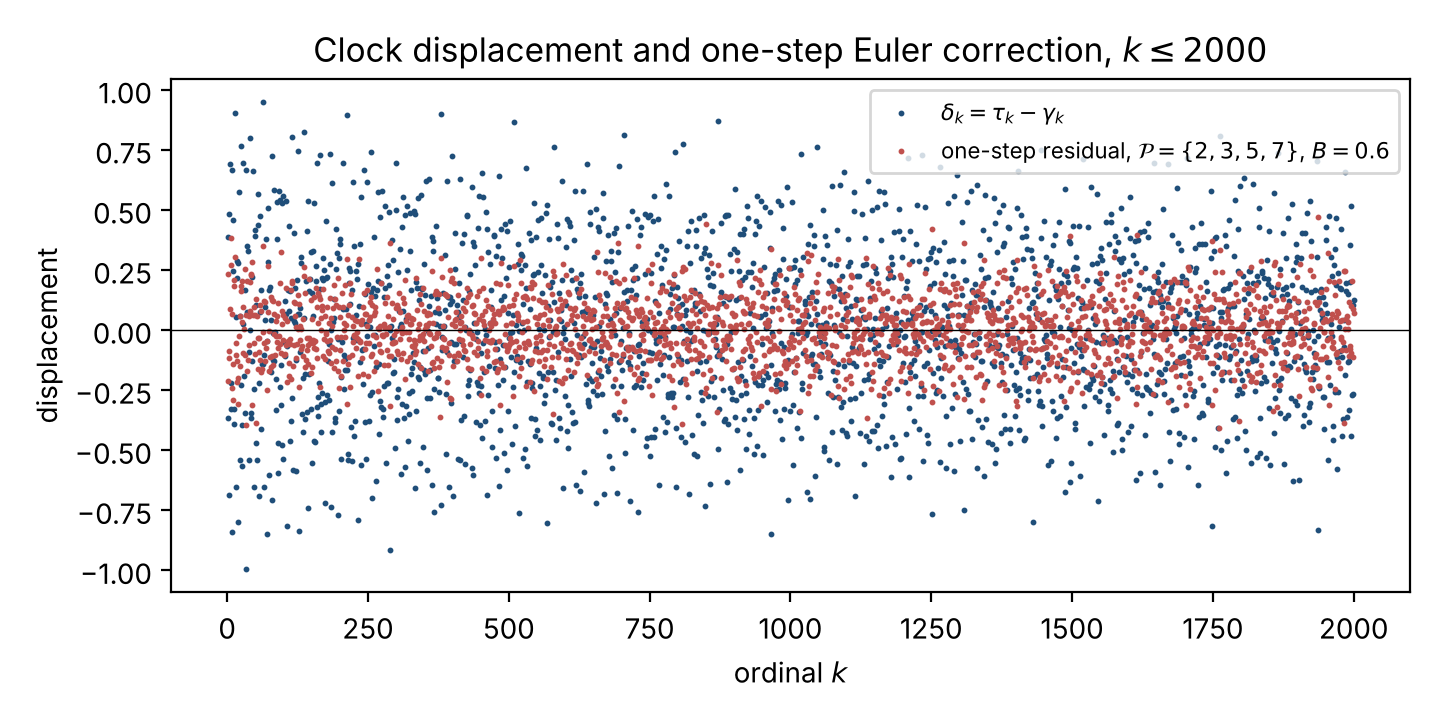
\includegraphics[width=0.92\textwidth]{fig01_displacement_first2000.png}
\caption{The displacement $\delta_k=\tau_k-\gamma_k$ and the residual of the one-step clock with $P=\{2,3,5,7\}$ and $B=0.6$, for $k\le2000$.}
\label{fig:displacement}
\end{figure}

\begin{figure}[htbp]
\centering
\includegraphics[width=0.92\textwidth]{fig02_rms_by_height.png}
\caption{RMS of the residual in logarithmic bins of $k$ for the five methods of Table~\CGref{tab:methods}.}
\label{fig:rms_height}
\end{figure}

\begin{figure}[htbp]
\centering
\includegraphics[width=0.92\textwidth]{fig08_max_by_window.png}
\caption{Maximum of $|$residual$|$ in each window for the five methods of Table~\CGref{tab:methods}; the dotted line is $\frac12$.}
\label{fig:max_window}
\end{figure}

\subsection{The optimal cutoff grows with the height}
\label{subsec:optimal_cutoff}

\begin{experiment}\label{exp:optimal_cutoff}
Object: RMS of $\delta_k^{X}$ (no saturation) as a function of the cutoff $X$, for $40$ cutoffs between $2$ and $1999$, and the minimizing cutoff in each window. Range: the six windows. Expected outcome: by Corollary~\CGref{cor:dichotomy} the cutoff should grow with the height; Heuristic~\CGref{heur:exponent} predicts an exponent $\theta$ slowly decreasing with the height. Observed outcome: Table~\CGref{tab:optimal_cutoff}, Figures~\CGref{fig:rms_cutoff} and \CGref{fig:optimal_cutoff}, and the full scan in Tables~\CGref{tab:scan_rms}--\CGref{tab:scan_max}. The optimal cutoff increases from $7$ to $907$; the least-squares fit $\log X_{\rm opt}=\theta\log(\tau/2\pi)$ over windows $2$--$6$ gives $\theta=0.5744$. Near the optimum the RMS curves are flat: in the top window the RMS is $0.064467$ at $X=701$, $0.064271$ at $X=907$ and $0.064283$ at $X=1009$. We observe that the exponent is not explained quantitatively by Heuristic~\CGref{heur:exponent} (Remark~\CGref{rem:negative_exponent}).
\end{experiment}

\begin{table}[htbp]
\centering
\small
\begin{tabular}{lrrrr}
\toprule
window & $X_{\rm opt}$ & RMS at $X_{\rm opt}$ & median $\log(\tau_k/2\pi)$ & RMS of $\delta_k$\\
\midrule
$(0,10^3]$ & 1e3] & 7 & 0.163507 & 4.8617\\
$(10^3,10^4]$ & 1e4] & 43 & 0.089165 & 6.8465\\
$(10^4,10^5]$ & 1e5] & 151 & 0.076935 & 8.8540\\
$(10^5,5\cdot10^5]$ & 5e5] & 401 & 0.069779 & 10.3736\\
$(5\cdot10^5,10^6]$ & 1e6] & 701 & 0.066360 & 11.2050\\
$(10^6,2001052]$ & 2001052] & 907 & 0.064271 & 11.8382\\
\bottomrule
\end{tabular}
\caption{RMS-optimal prime cutoff of the one-step clock (no saturation) in each window (Experiment~\CGref{exp:optimal_cutoff}).}
\label{tab:optimal_cutoff}
\end{table}

\begin{figure}[htbp]
\centering
\includegraphics[width=0.92\textwidth]{fig03_rms_vs_cutoff.png}
\caption{RMS of the one-step residual against the cutoff $X$ (primes $p\le X$, full local factors), by window; dots mark the minimum of each window.}
\label{fig:rms_cutoff}
\end{figure}

\begin{figure}[htbp]
\centering
\includegraphics[width=0.7\textwidth]{fig04_optimal_cutoff.png}
\caption{Logarithm of the optimal cutoff against the median of $\log(\tau_k/2\pi)$ in each window, with the least-squares line through the origin fitted on windows $2$--$6$.}
\label{fig:optimal_cutoff}
\end{figure}

\begin{experiment}\label{exp:saturation}
Object: global maximum of $|\delta_k^{X,B}|$, its location, the number of residuals $\ge\frac12$, the RMS, and the residual at $k=258318$, for the fixed cutoffs $11\le X\le71$ and $B\in\{0.5,0.6,0.7\}$. Range: $1\le k\le K$. Expected outcome: none from the theory, which says nothing about finite maxima (Proposition~\CGref{prop:fixed_sup} concerns the limit). Observed outcome: Table~\CGref{tab:saturation}. For $B=0.5$ and $X\ge13$ the maximum $0.493711$ at $k=34$ comes from the saturation itself: the bare residual there is $0.993711$. With $B=0.6$, the cutoffs $X\in\{13,17,31\}$ and all $37\le X\le71$ give a maximum below $\frac12$ over the $2\,001\,052$ zeros, the smallest being $0.457259$ for $X=61$.
\end{experiment}

\subsection{Mean-square gain and projections}
\label{subsec:gain_projection}

\begin{experiment}\label{exp:gain}
Object: the gain $\langle s_k^2\rangle-\langle(s_k-S_P(\tau_k))^2\rangle$ for $P=\{2,3,5,7\}$ and $P=\{p\le61\}$ with full local factors, compared with $c_P$ of \CGeqref{eq:cP_def}. Range: the six windows. Expected outcome: by Corollary~\CGref{cor:gain} and Remark~\CGref{rem:gain_full_factors} (conditional on Hypothesis~\CGref{hyp:L}), the gain of each finite truncation tends to its $v_A$, and $v_A\uparrow c_P$. Observed outcome: Table~\CGref{tab:gain} and Figure~\CGref{fig:gain}. The gain increases with the height towards $c_P$, from $0.056957$ to $0.064441$ for $c_P=0.066252$, and from $0.047822$ to $0.087434$ for $c_P=0.093853$. The mean square $\langle s_k^2\rangle$ increases from $0.067170$ to $0.113224$, as Theorem~\CGref{thm:clock_moments} predicts qualitatively; the theorem determines only the leading term $(2\pi^2)^{-1}\log\log T$ and not the constant.
\end{experiment}

\begin{table}[htbp]
\centering
\small
\begin{tabular}{lrrrrr}
\toprule
window & $\langle s_k^2\rangle$ & gain, $P_7$ & $c_{P_7}$ & gain, $P_{61}$ & $c_{P_{61}}$\\
\midrule
$(0,10^3]$ & 1e3] & 0.067170 & 0.056957 & 0.066252 & 0.047822\\
$(10^3,10^4]$ & 1e4] & 0.085195 & 0.063224 & 0.066252 & 0.075868\\
$(10^4,10^5]$ & 1e5] & 0.098097 & 0.063878 & 0.066252 & 0.084636\\
$(10^5,5\cdot10^5]$ & 5e5] & 0.106325 & 0.064185 & 0.066252 & 0.086367\\
$(5\cdot10^5,10^6]$ & 1e6] & 0.110476 & 0.064339 & 0.066252 & 0.087027\\
$(10^6,2001052]$ & 2001052] & 0.113224 & 0.064441 & 0.066252 & 0.087434\\
\bottomrule
\end{tabular}
\caption{Mean-square gain of a fixed Euler phase against its limit $c_P$; $P_7=\{2,3,5,7\}$, $P_{61}=\{p\le61\}$ (Experiment~\CGref{exp:gain}).}
\label{tab:gain}
\end{table}

\begin{figure}[htbp]
\centering
\includegraphics[width=0.92\textwidth]{fig07_gain_vs_theory.png}
\caption{Measured mean-square gain of a fixed Euler phase in each window (markers) and the constants $c_P$ (dashed).}
\label{fig:gain}
\end{figure}

\begin{experiment}\label{exp:projection}
Object: the normalized projections $\rho_n=-2\pi\sqrt n\,\langle s_k\sin(\tau_k\log n)\rangle$ for $2\le n\le64$. Range: $10^6<k\le K$, where the median of $\log(\tau_k/2\pi)$ is $11.8382$. Expected outcome: $\rho_n\to\Lambda(n)/\log n$ by Theorem~\CGref{thm:projection} (conditional on Hypothesis~\CGref{hyp:L}), with the second-order correction \CGeqref{eq:second_order} at finite height (Heuristic~\CGref{heur:second_order}). Observed outcome: Table~\CGref{tab:projection} and Figure~\CGref{fig:projection}. For primes $\rho_p$ lies between $0.864$ and $0.979$; for prime squares between $0.526$ and $0.576$; over $n=p^aq^b\le64$ the largest deviation from \CGeqref{eq:second_order} is $0.0632$; the largest $|\rho_n|$ over integers which are not prime powers is $0.2936$, and the largest deviation from $\Lambda(n)/\log n$ over prime powers is $0.1356$.
\end{experiment}

\begin{figure}[htbp]
\centering
\includegraphics[width=0.92\textwidth]{fig05_projection_coefficients.png}
\caption{Normalized projections $\rho_n$ of the displacement on $\sin(\tau_k\log n)$, $10^6<k\le K$, with the first-order limit $\Lambda(n)/\log n$ and the second-order prediction \CGeqref{eq:second_order}.}
\label{fig:projection}
\end{figure}

\subsection{The extreme residual: a close pair of zeros}
\label{subsec:close_pair}

\begin{experiment}\label{exp:close_pair}
Object: the zero at which the fixed set $P=\{2,3,5,7\}$ with $B=0.6$ attains its largest residual. Range: $258315\le k\le258321$. Expected outcome: a large $|s_k|$, which by \CGeqref{eq:sawtooth_sandwich} forces a large value of $|S|$ nearby. Observed outcome: Table~\CGref{tab:close_pair} and Figure~\CGref{fig:close_pair}. The ordinates $\gamma_{258317}=175681.649131916$ and $\gamma_{258318}=175681.715894456$ form a close pair with normalized gap $0.1088$ (rank $2371$ among $2\,001\,051$ gaps), followed by a normalized gap $2.6587$. The midpoint value is $S(\gamma_{258318})=1.0394$ and $\delta_{258318}=0.6379$. The residuals at $k=258318$ are $0.5223$ ($P=\{2,3,5,7\}$, $B=0.6$), $0.2345$ ($P=\{p\le61\}$, $B=0.6$), $0.3373$ ($P=\{p\le1999\}$) and $0.2031$ (ordinal-dependent cutoff).
\end{experiment}

\begin{table}[htbp]
\centering
\small
\begin{tabular}{rrrrrr}
\toprule
$k$ & $\gamma_k$ & $\tau_k$ & $\delta_k$ & $\gamma_{k+1}-\gamma_k$ & normalized gap\\
\midrule
258315 & 175680.155201189 & 175680.512721900 & $+0.3575$ & 0.8010 & 1.3053\\
258316 & 175680.956210354 & 175681.126401291 & $+0.1702$ & 0.6929 & 1.1291\\
258317 & 175681.649131916 & 175681.740080472 & $+0.0909$ & 0.0668 & 0.1088\\
258318 & 175681.715894456 & 175682.353759444 & $+0.6379$ & 1.6316 & 2.6587\\
258319 & 175683.347455659 & 175682.967438207 & $-0.3800$ & 0.5181 & 0.8443\\
258320 & 175683.865589247 & 175683.581116760 & $-0.2845$ & 0.4856 & 0.7914\\
258321 & 175684.351235152 & 175684.194795104 & $-0.1564$ & 0.3002 & 0.4892\\
\bottomrule
\end{tabular}
\caption{Ordinates, clock and gaps around the close pair $k=258317,258318$; the normalized gap is $(\gamma_{k+1}-\gamma_k)\log(\gamma_k/2\pi)/2\pi$ (Experiment~\CGref{exp:close_pair}).}
\label{tab:close_pair}
\end{table}

\begin{figure}[htbp]
\centering
\includegraphics[width=0.92\textwidth]{fig06_close_pair.png}
\caption{Zeros, clock and one-step clocks around the close pair $k=258317,258318$.}
\label{fig:close_pair}
\end{figure}

\section{Discussion}
\label{sec:discussion}

\subsection{Status of the results}
\label{subsec:status}
Theorems~\CGref{thm:identity_general}, \CGref{thm:clock_moments} and \CGref{thm:main}, their corollaries, and Propositions~\CGref{prop:extremes}, \CGref{prop:fixed_sup}, \CGref{prop:localization} and \CGref{prop:one_step_decomposition} are unconditional. Theorem~\CGref{thm:projection} and Corollary~\CGref{cor:gain} assume Hypothesis~\CGref{hyp:L}, which follows from the Riemann hypothesis. Heuristics~\CGref{heur:exponent} and \CGref{heur:second_order} are heuristic. The value $0.57$ of the exponent and all statements about finite maxima are numerical observations.

\subsection{What is proved about the improvement}
\label{subsec:what_proved}
Theorem~\CGref{thm:main} answers the question whether a number of primes depending on the ordinal improves the truncated Fran\c{c}a--LeClair equation, in the mean-square sense and for the equation itself: a fixed number of primes leaves a defect whose mean square grows like $(2\pi^2)^{-1}\log\log T$, a cutoff $X=T^c$ keeps it bounded, and boundedness requires $\log X\asymp\log T$. The power law is therefore forced by the theorem; the value of the exponent is not. Within $0<c\le\frac12$ the bound \CGeqref{eq:main_theorem} decreases with $c$, which suggests taking $c$ as large as the method allows for the equation itself. For the one-step clock, which evaluates the phase at $\tau_k$, the optimal exponent results from a balance described by Heuristic~\CGref{heur:exponent}, and no theorem is proved.

The sup norm behaves differently. In the $t$-variable, $\limsup|\delta_k|\le0.6331$ unconditionally and $\delta_k\to0$ on the Riemann hypothesis (Proposition~\CGref{prop:extremes}); a fixed set of primes changes no limit superior (Proposition~\CGref{prop:fixed_sup}). The improvement of finite maxima seen in Experiment~\CGref{exp:saturation} is therefore a phenomenon at finite height.

\subsection{Novelty}
\label{subsec:novelty}
Selberg's approximation of $S(t)$ by prime sums up to a power of $T$ is a statement on $t$-averages and is due to Selberg; Selberg and Korolev treat the integer displacement from Gram intervals (Remark~\CGref{rem:korolev}). We have not found in the literature we consulted the identity of Theorem~\CGref{thm:identity_general}, the mean-square theorem for the defect at the zeros (Theorem~\CGref{thm:main}) or the dichotomy of Corollary~\CGref{cor:dichotomy}; the absence of results in a search is weak evidence, and these statements may have antecedents that we missed. In \cite{LeClair2021} the number of primes is subject to $N(t)\to\infty$ and $N<[t^2]$, without a rule selecting it from the ordinal, and the truncated equation is supported by a probabilistic model; we found no proof of its validity in \cite{FrancaLeClair2014,FrancaLeClair2015,LeClair2021}. For finite Euler products near the critical line in a different direction see Gonek \cite{Gonek2012}.

\begin{remark}\label{rem:no_spacing}
The results proved here concern the arithmetic part of the displacement, of size $\sqrt{\log\log T}$, and its removal by primes; they do not address the local spacing statistics of the zeros. For instance, replacing each $\gamma_k$ by $\gamma_k+\epsilon_k$ with $|\epsilon_k|\le\epsilon/\lL(\gamma_k)$ changes each $s_k$ by at most $\epsilon(1+o(1))$, hence the root mean square in Theorem~\CGref{thm:clock_moments} by at most $\epsilon(1+o(1))$, whatever the local statistics of the perturbed sequence. In particular Theorem~\CGref{thm:clock_moments} does not imply random matrix statistics for the zeros.
\end{remark}

\section{Open questions and future work}
\label{sec:open_questions}

\begin{question}\label{q:constant}
Does $\frac1{\#\IT}\sum_{k\in\IT}u_k(T^c)^2=\frac1{2\pi^2}\log\frac1c+\kappa+o(1)$ hold for fixed $c\in(0,\frac12]$, with an explicit constant $\kappa$?
\end{question}

\begin{question}\label{q:large_c}
Does Theorem~\CGref{thm:main} extend to $\frac12<c\le2$, which contains LeClair's range $N<[t^2]$? The proof uses $X^2\le T$ in the fourth-moment step of Lemma~\CGref{lem:D_moments}.
\end{question}

\begin{question}\label{q:per_ordinate}
Does \CGeqref{eq:main_theorem} hold for cutoffs $X_k=(\tau_k/2\pi)^\theta$ that vary from zero to zero? This needs a maximal inequality for partial sums of $S_X$ at the zeros.
\end{question}

\begin{question}\label{q:one_step}
Is the mean square of the one-step residual $r_k(T^c)$ asymptotic to $c^2(2\pi^2)^{-1}\log\log T$ for fixed $c$, as Heuristic~\CGref{heur:exponent} suggests, and what is the optimal exponent $\theta(T)$ of the one-step clock?
\end{question}

\begin{question}\label{q:experiment_uk}
Future experiment: compute $u_k(X)$ for $X=2^{rc}$ on the windows $\mathcal I_{2^r}$ and compare with \CGeqref{eq:main_theorem}; compute the solutions of $F_X(t)=k-\frac12$ by Newton's method for $X\ll\log^2T$ and compare with Proposition~\CGref{prop:localization}.
\end{question}

\begin{question}\label{q:generalization}
Possible generalization: Dirichlet $L$-functions, for which Fran\c{c}a and LeClair give the analogous equation \cite{FrancaLeClair2015} and Selberg's approximation is available in the form of \cite[\S3]{Fujii1974} for primitive characters.
\end{question}

\appendix

\section{Complete tables}
\label{sec:appendix_tables}

\begin{center}
\small
\begin{longtable}{rrrrrrr}
\caption{RMS of $\delta_k^X$ (no saturation) for all cutoffs of the scan of Experiment~\CGref{exp:optimal_cutoff}.}\label{tab:scan_rms}\\
\toprule
$X$ & $(0,10^3]$ & $(10^3,10^4]$ & $(10^4,10^5]$ & $(10^5,5\cdot10^5]$ & $(5\cdot10^5,10^6]$ & $(10^6,K]$\\
\midrule
\endfirsthead
\toprule
$X$ & $(0,10^3]$ & $(10^3,10^4]$ & $(10^4,10^5]$ & $(10^5,5\cdot10^5]$ & $(5\cdot10^5,10^6]$ & $(10^6,K]$\\
\midrule
\endhead
2 & 0.264585 & 0.221853 & 0.189628 & 0.169743 & 0.160181 & 0.154125\\
3 & 0.200546 & 0.182692 & 0.162903 & 0.148543 & 0.141254 & 0.136519\\
5 & 0.175536 & 0.157325 & 0.145975 & 0.135250 & 0.129435 & 0.125551\\
7 & 0.163507 & 0.138018 & 0.133227 & 0.125335 & 0.120648 & 0.117413\\
11 & 0.167491 & 0.125933 & 0.125019 & 0.118978 & 0.115014 & 0.112199\\
13 & 0.180112 & 0.115143 & 0.117861 & 0.113445 & 0.110121 & 0.107676\\
17 & 0.189732 & 0.107018 & 0.112357 & 0.109187 & 0.106362 & 0.104196\\
19 & 0.203848 & 0.099967 & 0.107341 & 0.105291 & 0.102932 & 0.101027\\
23 & 0.207822 & 0.094970 & 0.103192 & 0.102058 & 0.100080 & 0.098398\\
29 & 0.220519 & 0.091980 & 0.099933 & 0.099516 & 0.097835 & 0.096324\\
31 & 0.230788 & 0.089845 & 0.096818 & 0.097113 & 0.095707 & 0.094360\\
37 & 0.233278 & 0.089201 & 0.094209 & 0.095126 & 0.093936 & 0.092724\\
43 & 0.247108 & 0.089165 & 0.089653 & 0.091595 & 0.090813 & 0.089816\\
53 & 0.253280 & 0.090105 & 0.085984 & 0.088604 & 0.088177 & 0.087369\\
61 & 0.261896 & 0.091200 & 0.083253 & 0.086131 & 0.085995 & 0.085356\\
71 & 0.272840 & 0.092404 & 0.081157 & 0.083975 & 0.084099 & 0.083607\\
83 & 0.279043 & 0.094679 & 0.078846 & 0.081114 & 0.081573 & 0.081281\\
97 & 0.279760 & 0.096097 & 0.077984 & 0.079519 & 0.080174 & 0.079986\\
113 & 0.305237 & 0.099735 & 0.077086 & 0.076058 & 0.077117 & 0.077155\\
131 & 0.303814 & 0.101313 & 0.076968 & 0.075024 & 0.076116 & 0.076235\\
151 & 0.309424 & 0.104066 & 0.076935 & 0.073336 & 0.074335 & 0.074579\\
173 & 0.323001 & 0.106809 & 0.077044 & 0.072094 & 0.072794 & 0.073149\\
199 & 0.322057 & 0.110538 & 0.077336 & 0.070915 & 0.070796 & 0.071304\\
229 & 0.322766 & 0.112658 & 0.077638 & 0.070557 & 0.069704 & 0.070261\\
263 & 0.335293 & 0.115531 & 0.078195 & 0.070231 & 0.068448 & 0.068864\\
307 & 0.339800 & 0.119016 & 0.078840 & 0.069985 & 0.067633 & 0.067458\\
353 & 0.342957 & 0.122519 & 0.079635 & 0.069831 & 0.067253 & 0.066262\\
401 & 0.358302 & 0.125367 & 0.080542 & 0.069779 & 0.066961 & 0.065561\\
461 & 0.359151 & 0.128498 & 0.081570 & 0.069855 & 0.066669 & 0.065176\\
523 & 0.354759 & 0.131831 & 0.082601 & 0.069960 & 0.066526 & 0.064877\\
601 & 0.367055 & 0.134709 & 0.083735 & 0.070147 & 0.066431 & 0.064663\\
701 & 0.376638 & 0.138525 & 0.085322 & 0.070484 & 0.066360 & 0.064467\\
809 & 0.367728 & 0.141873 & 0.086526 & 0.070817 & 0.066390 & 0.064353\\
907 & 0.377272 & 0.144454 & 0.087902 & 0.071167 & 0.066521 & 0.064271\\
1009 & 0.387648 & 0.146798 & 0.089073 & 0.071525 & 0.066595 & 0.064283\\
1201 & 0.378526 & 0.151049 & 0.091182 & 0.072272 & 0.066845 & 0.064317\\
1409 & 0.381402 & 0.154503 & 0.092992 & 0.072896 & 0.067167 & 0.064412\\
1601 & 0.399367 & 0.158134 & 0.094832 & 0.073618 & 0.067469 & 0.064584\\
1801 & 0.389913 & 0.161587 & 0.096305 & 0.074283 & 0.067767 & 0.064768\\
1999 & 0.384555 & 0.163764 & 0.097502 & 0.074828 & 0.068088 & 0.064897\\
\bottomrule
\end{longtable}
\end{center}

\begin{center}
\small
\begin{longtable}{rrrrrrr}
\caption{Maximum of $|\delta_k^X|$ (no saturation) for all cutoffs of the scan of Experiment~\CGref{exp:optimal_cutoff}.}\label{tab:scan_max}\\
\toprule
$X$ & $(0,10^3]$ & $(10^3,10^4]$ & $(10^4,10^5]$ & $(10^5,5\cdot10^5]$ & $(5\cdot10^5,10^6]$ & $(10^6,K]$\\
\midrule
\endfirsthead
\toprule
$X$ & $(0,10^3]$ & $(10^3,10^4]$ & $(10^4,10^5]$ & $(10^5,5\cdot10^5]$ & $(5\cdot10^5,10^6]$ & $(10^6,K]$\\
\midrule
\endhead
2 & 0.714732 & 0.769491 & 0.692832 & 0.720658 & 0.661936 & 0.671779\\
3 & 0.778082 & 0.590169 & 0.597440 & 0.601584 & 0.561789 & 0.568719\\
5 & 1.374655 & 0.516964 & 0.542554 & 0.529087 & 0.499111 & 0.519284\\
7 & 1.363459 & 0.470967 & 0.477838 & 0.522347 & 0.484035 & 0.489293\\
11 & 1.508302 & 0.509751 & 0.476272 & 0.484013 & 0.461281 & 0.472383\\
13 & 1.890769 & 0.471351 & 0.485959 & 0.459791 & 0.471622 & 0.445972\\
17 & 2.030160 & 0.462473 & 0.484965 & 0.471862 & 0.452001 & 0.438833\\
19 & 2.579012 & 0.511457 & 0.473939 & 0.436459 & 0.420326 & 0.419404\\
23 & 2.086207 & 0.480575 & 0.516961 & 0.449248 & 0.426305 & 0.396139\\
29 & 2.532059 & 0.517976 & 0.486233 & 0.456782 & 0.425924 & 0.421632\\
31 & 2.731378 & 0.478395 & 0.503207 & 0.436347 & 0.394374 & 0.408531\\
37 & 2.436264 & 0.472277 & 0.467938 & 0.457662 & 0.402816 & 0.408334\\
43 & 2.920237 & 0.445443 & 0.482769 & 0.454351 & 0.425856 & 0.418435\\
53 & 2.844272 & 0.421161 & 0.474280 & 0.499673 & 0.435596 & 0.405677\\
61 & 2.717402 & 0.386775 & 0.457259 & 0.456272 & 0.432954 & 0.400144\\
71 & 3.238857 & 0.440040 & 0.447583 & 0.474087 & 0.436888 & 0.399374\\
83 & 2.963768 & 0.484372 & 0.467632 & 0.463983 & 0.438356 & 0.404333\\
97 & 2.894415 & 0.492464 & 0.483027 & 0.471593 & 0.460266 & 0.426854\\
113 & 3.849430 & 0.505889 & 0.513140 & 0.459718 & 0.483898 & 0.444630\\
131 & 3.439317 & 0.529451 & 0.517859 & 0.460881 & 0.484771 & 0.422286\\
151 & 3.367629 & 0.513247 & 0.525446 & 0.470577 & 0.482027 & 0.452456\\
173 & 3.996564 & 0.501890 & 0.549235 & 0.495148 & 0.456277 & 0.461665\\
199 & 3.365175 & 0.506558 & 0.523619 & 0.495310 & 0.458465 & 0.468141\\
229 & 3.335133 & 0.493618 & 0.528107 & 0.497048 & 0.468220 & 0.469958\\
263 & 4.072437 & 0.509804 & 0.557233 & 0.535397 & 0.479418 & 0.457026\\
307 & 3.875649 & 0.526799 & 0.546887 & 0.526425 & 0.467465 & 0.473187\\
353 & 3.465466 & 0.541694 & 0.561048 & 0.534833 & 0.473423 & 0.477070\\
401 & 4.309564 & 0.517594 & 0.555640 & 0.563591 & 0.504123 & 0.520443\\
461 & 4.028754 & 0.524278 & 0.544453 & 0.564897 & 0.521484 & 0.515423\\
523 & 3.255435 & 0.547997 & 0.577784 & 0.573315 & 0.492713 & 0.513253\\
601 & 4.111242 & 0.510670 & 0.585122 & 0.569968 & 0.507595 & 0.499887\\
701 & 4.359529 & 0.561843 & 0.576930 & 0.548586 & 0.495677 & 0.503530\\
809 & 3.399704 & 0.551479 & 0.599065 & 0.553709 & 0.486320 & 0.525568\\
907 & 4.022965 & 0.520528 & 0.588646 & 0.540603 & 0.524873 & 0.529711\\
1009 & 4.759390 & 0.506597 & 0.574853 & 0.553235 & 0.523729 & 0.521027\\
1201 & 3.414545 & 0.491973 & 0.602652 & 0.560114 & 0.551342 & 0.534354\\
1409 & 3.934751 & 0.472026 & 0.587566 & 0.572365 & 0.566273 & 0.533096\\
1601 & 4.812450 & 0.524598 & 0.593689 & 0.572861 & 0.554297 & 0.526446\\
1801 & 3.551103 & 0.528815 & 0.586851 & 0.576451 & 0.554530 & 0.526215\\
1999 & 3.247397 & 0.491263 & 0.618127 & 0.591452 & 0.552165 & 0.528267\\
\bottomrule
\end{longtable}
\end{center}

\begin{center}
\small
\begin{longtable}{rrrrrrr}
\caption{Fixed cutoffs and saturation levels over all $K$ zeros (Experiment~\CGref{exp:saturation}).}\label{tab:saturation}\\
\toprule
$X$ & $B$ & global max & $k$ at max & $\#\ge\frac12$ & RMS & residual at $k=258318$\\
\midrule
\endfirsthead
\toprule
$X$ & $B$ & global max & $k$ at max & $\#\ge\frac12$ & RMS & residual at $k=258318$\\
\midrule
\endhead
11 & 0.5 & 0.497093 & 1252 & 0 & 0.114954 & +0.468830\\
11 & 0.6 & 0.509751 & 1252 & 1 & 0.114954 & +0.468830\\
11 & 0.7 & 0.509751 & 1252 & 1 & 0.114954 & +0.468830\\
13 & 0.5 & 0.493711 & 34 & 0 & 0.109968 & +0.414562\\
13 & 0.6 & 0.485959 & 28074 & 0 & 0.109974 & +0.414562\\
13 & 0.7 & 0.485959 & 28074 & 0 & 0.109975 & +0.414562\\
17 & 0.5 & 0.493711 & 34 & 0 & 0.106136 & +0.377680\\
17 & 0.6 & 0.484965 & 28075 & 0 & 0.106150 & +0.377680\\
17 & 0.7 & 0.484965 & 28075 & 0 & 0.106153 & +0.377680\\
19 & 0.5 & 0.493711 & 34 & 0 & 0.102639 & +0.351715\\
19 & 0.6 & 0.511457 & 4988 & 1 & 0.102665 & +0.351715\\
19 & 0.7 & 0.511457 & 4988 & 1 & 0.102670 & +0.351715\\
23 & 0.5 & 0.493711 & 34 & 0 & 0.099739 & +0.321005\\
23 & 0.6 & 0.516961 & 28075 & 1 & 0.099777 & +0.321005\\
23 & 0.7 & 0.516961 & 28075 & 1 & 0.099784 & +0.321005\\
29 & 0.5 & 0.493711 & 34 & 0 & 0.097456 & +0.320746\\
29 & 0.6 & 0.517976 & 4988 & 1 & 0.097509 & +0.320746\\
29 & 0.7 & 0.517976 & 4988 & 1 & 0.097518 & +0.320746\\
31 & 0.5 & 0.493711 & 34 & 0 & 0.095297 & +0.286603\\
31 & 0.6 & 0.481293 & 28075 & 0 & 0.095364 & +0.286603\\
31 & 0.7 & 0.503207 & 31812 & 1 & 0.095375 & +0.286603\\
37 & 0.5 & 0.493711 & 34 & 0 & 0.093503 & +0.257718\\
37 & 0.6 & 0.472277 & 6709 & 0 & 0.093584 & +0.257718\\
37 & 0.7 & 0.481833 & 7 & 0 & 0.093598 & +0.257718\\
41 & 0.5 & 0.493711 & 34 & 0 & 0.091884 & +0.282516\\
41 & 0.6 & 0.480998 & 5444 & 0 & 0.091977 & +0.282516\\
41 & 0.7 & 0.481833 & 7 & 0 & 0.091994 & +0.282516\\
43 & 0.5 & 0.493711 & 34 & 0 & 0.090330 & +0.255696\\
43 & 0.6 & 0.482769 & 55259 & 0 & 0.090438 & +0.255696\\
43 & 0.7 & 0.482769 & 55259 & 0 & 0.090456 & +0.255696\\
47 & 0.5 & 0.493711 & 34 & 0 & 0.088909 & +0.233942\\
47 & 0.6 & 0.477323 & 30265 & 0 & 0.089031 & +0.233942\\
47 & 0.7 & 0.489035 & 31812 & 0 & 0.089052 & +0.233942\\
53 & 0.5 & 0.493711 & 34 & 0 & 0.087660 & +0.260451\\
53 & 0.6 & 0.474829 & 100674 & 0 & 0.087797 & +0.260451\\
53 & 0.7 & 0.499673 & 100674 & 0 & 0.087821 & +0.260451\\
59 & 0.5 & 0.493711 & 34 & 0 & 0.086551 & +0.239402\\
59 & 0.6 & 0.474829 & 100674 & 0 & 0.086700 & +0.239402\\
59 & 0.7 & 0.482408 & 100674 & 0 & 0.086726 & +0.239402\\
61 & 0.5 & 0.493711 & 34 & 0 & 0.085471 & +0.234496\\
61 & 0.6 & 0.457259 & 55259 & 0 & 0.085635 & +0.234496\\
61 & 0.7 & 0.481833 & 7 & 0 & 0.085663 & +0.234496\\
67 & 0.5 & 0.493711 & 34 & 0 & 0.084496 & +0.258256\\
67 & 0.6 & 0.474829 & 100674 & 0 & 0.084673 & +0.258256\\
67 & 0.7 & 0.481833 & 7 & 0 & 0.084704 & +0.258256\\
71 & 0.5 & 0.493711 & 34 & 0 & 0.083579 & +0.248477\\
71 & 0.6 & 0.458509 & 100674 & 0 & 0.083769 & +0.248477\\
71 & 0.7 & 0.481833 & 7 & 0 & 0.083803 & +0.248477\\
\bottomrule
\end{longtable}
\end{center}

\begin{center}
\small
\begin{longtable}{rrrrr}
\caption{Projections of the displacement, $10^6<k\le K$ (Experiment~\CGref{exp:projection}). Columns: $n$; $\langle\lL(\tau_k)\delta_k\sin(\tau_k\log n)\rangle$; $\rho_n$; $\Lambda(n)/\log n$; second-order prediction $\log n/(ab\log(\tau/2\pi))$ for $n=p^aq^b$ with the median of $\log(\tau_k/2\pi)$.}\label{tab:projection}\\
\toprule
$n$ & projection & $\rho_n$ & $\Lambda(n)/\log n$ & second order\\
\midrule
\endfirsthead
\toprule
$n$ & projection & $\rho_n$ & $\Lambda(n)/\log n$ & second order\\
\midrule
\endhead
2 & $-1.101798\cdot10^{-1}$ & 0.979032 & 1.000000 & --\\
3 & $-8.948284\cdot10^{-2}$ & 0.973824 & 1.000000 & --\\
4 & $-4.184672\cdot10^{-2}$ & 0.525861 & 0.500000 & --\\
5 & $-6.870881\cdot10^{-2}$ & 0.965333 & 1.000000 & --\\
6 & $-9.026866\cdot10^{-3}$ & 0.138929 & 0.000000 & 0.151353\\
7 & $-5.760368\cdot10^{-2}$ & 0.957589 & 1.000000 & --\\
8 & $-2.155326\cdot10^{-2}$ & 0.383035 & 0.333333 & --\\
9 & $-2.905212\cdot10^{-2}$ & 0.547620 & 0.500000 & --\\
10 & $-8.834723\cdot10^{-3}$ & 0.175539 & 0.000000 & 0.194504\\
11 & $-4.529915\cdot10^{-2}$ & 0.943987 & 1.000000 & --\\
12 & $-5.057500\cdot10^{-3}$ & 0.110079 & 0.000000 & 0.104952\\
13 & $-4.140890\cdot10^{-2}$ & 0.938092 & 1.000000 & --\\
14 & $-8.442033\cdot10^{-3}$ & 0.198468 & 0.000000 & 0.222926\\
15 & $-8.499428\cdot10^{-3}$ & 0.206831 & 0.000000 & 0.228754\\
16 & $-1.262904\cdot10^{-2}$ & 0.317402 & 0.250000 & --\\
17 & $-3.580933\cdot10^{-2}$ & 0.927685 & 1.000000 & --\\
18 & $-4.855880\cdot10^{-3}$ & 0.129445 & 0.000000 & 0.122078\\
19 & $-3.369338\cdot10^{-2}$ & 0.922787 & 1.000000 & --\\
20 & $-4.806896\cdot10^{-3}$ & 0.135070 & 0.000000 & 0.126528\\
21 & $-7.977501\cdot10^{-3}$ & 0.229698 & 0.000000 & 0.257177\\
22 & $-7.712575\cdot10^{-3}$ & 0.227295 & 0.000000 & 0.261106\\
23 & $-3.034556\cdot10^{-2}$ & 0.914406 & 1.000000 & --\\
24 & $-3.431327\cdot10^{-3}$ & 0.105620 & 0.000000 & 0.089486\\
25 & $-1.807767\cdot10^{-2}$ & 0.567927 & 0.500000 & --\\
26 & $-7.409792\cdot10^{-3}$ & 0.237396 & 0.000000 & 0.275218\\
27 & $-1.284469\cdot10^{-2}$ & 0.419359 & 0.333333 & --\\
28 & $-4.547679\cdot10^{-3}$ & 0.151199 & 0.000000 & 0.140739\\
29 & $-2.670938\cdot10^{-2}$ & 0.903738 & 1.000000 & --\\
30 & $-1.996010\cdot10^{-3}$ & 0.068692 & 0.000000 & --\\
31 & $-2.574513\cdot10^{-2}$ & 0.900649 & 1.000000 & --\\
32 & $-7.950979\cdot10^{-3}$ & 0.282602 & 0.200000 & --\\
33 & $-7.157940\cdot10^{-3}$ & 0.258360 & 0.000000 & 0.295357\\
34 & $-6.894815\cdot10^{-3}$ & 0.252605 & 0.000000 & 0.297879\\
35 & $-7.143158\cdot10^{-3}$ & 0.265524 & 0.000000 & 0.300327\\
36 & $-2.718760\cdot10^{-3}$ & 0.102495 & 0.000000 & 0.075677\\
37 & $-2.332464\cdot10^{-2}$ & 0.891447 & 1.000000 & --\\
38 & $-6.689950\cdot10^{-3}$ & 0.259116 & 0.000000 & 0.307274\\
39 & $-6.836467\cdot10^{-3}$ & 0.268253 & 0.000000 & 0.309468\\
40 & $-3.176432\cdot10^{-3}$ & 0.126226 & 0.000000 & 0.103869\\
41 & $-2.204080\cdot10^{-2}$ & 0.886746 & 1.000000 & --\\
42 & $-2.004407\cdot10^{-3}$ & 0.081619 & 0.000000 & --\\
43 & $-2.145466\cdot10^{-2}$ & 0.883966 & 1.000000 & --\\
44 & $-4.148809\cdot10^{-3}$ & 0.172914 & 0.000000 & 0.159829\\
45 & $-4.254161\cdot10^{-3}$ & 0.179308 & 0.000000 & 0.160778\\
46 & $-6.334462\cdot10^{-3}$ & 0.269941 & 0.000000 & 0.323413\\
47 & $-2.040786\cdot10^{-2}$ & 0.879076 & 1.000000 & --\\
48 & $-2.483491\cdot10^{-3}$ & 0.108109 & 0.000000 & 0.081752\\
49 & $-1.309455\cdot10^{-2}$ & 0.575928 & 0.500000 & --\\
50 & $-4.016163\cdot10^{-3}$ & 0.178433 & 0.000000 & 0.165228\\
51 & $-6.336008\cdot10^{-3}$ & 0.284303 & 0.000000 & 0.332129\\
52 & $-3.977664\cdot10^{-3}$ & 0.180223 & 0.000000 & 0.166885\\
53 & $-1.907514\cdot10^{-2}$ & 0.872540 & 1.000000 & --\\
54 & $-2.978449\cdot10^{-3}$ & 0.137520 & 0.000000 & 0.112319\\
55 & $-6.301149\cdot10^{-3}$ & 0.293617 & 0.000000 & 0.338507\\
56 & $-3.008650\cdot10^{-3}$ & 0.141464 & 0.000000 & 0.113343\\
57 & $-6.113419\cdot10^{-3}$ & 0.290002 & 0.000000 & 0.341525\\
58 & $-5.863989\cdot10^{-3}$ & 0.280600 & 0.000000 & 0.342994\\
59 & $-1.796165\cdot10^{-2}$ & 0.866866 & 1.000000 & --\\
60 & $-1.282342\cdot10^{-3}$ & 0.062411 & 0.000000 & --\\
61 & $-1.761495\cdot10^{-2}$ & 0.864423 & 1.000000 & --\\
62 & $-5.768611\cdot10^{-3}$ & 0.285395 & 0.000000 & 0.348627\\
63 & $-3.940823\cdot10^{-3}$ & 0.196534 & 0.000000 & 0.174989\\
64 & $-5.250276\cdot10^{-3}$ & 0.263908 & 0.166667 & --\\
\bottomrule
\end{longtable}
\end{center}

\section{Reproducibility}
\label{sec:reproducibility}
The repository accompanying this paper contains \texttt{code/opc\_analysis.py} (Python~3 with NumPy, SciPy, Matplotlib and mpmath), which produces every table and figure of Section~\CGref{sec:numerical_experiments} in about one minute and is reproduced in full in Appendix~\CGref{sec:python_code} after the bibliography, the outputs in \texttt{outputs/}, and the figures in \texttt{figures/}. The data files \texttt{zeross.bin} (ordinates) and \texttt{zLamb.bin} (clock), each $2\,001\,052$ little-endian double-precision numbers, are not included in the repository because of their size; they are expected in \texttt{data/}.

\begin{thebibliography}{99}

\bibitem{BellottiWong2025}
C.~Bellotti and P.-J. Wong, Improved estimates for the argument and zero-counting function of the Riemann zeta-function, \emph{Math. Comp.} (2025, published online), \href{https://doi.org/10.1090/mcom/4133}{doi:10.1090/mcom/4133}; arXiv:2412.15470.

\bibitem{Billingsley1995}
P.~Billingsley, \emph{Probability and Measure}, 3rd ed., Wiley, New York, 1995. (No DOI.)

\bibitem{Corless1996}
R.~M. Corless, G.~H. Gonnet, D.~E.~G. Hare, D.~J. Jeffrey and D.~E. Knuth, On the Lambert $W$ function, \emph{Adv. Comput. Math.} \textbf{5} (1996), 329--359, \href{https://doi.org/10.1007/BF02124750}{doi:10.1007/BF02124750}.

\bibitem{FrancaLeClair2014}
G.~Fran\c{c}a and A.~LeClair, Statistical and other properties of Riemann zeros based on an explicit equation for the $n$-th zero on the critical line, preprint, arXiv:1307.8395 (2013), \href{https://doi.org/10.48550/arXiv.1307.8395}{doi:10.48550/arXiv.1307.8395}.

\bibitem{FrancaLeClair2015}
G.~Fran\c{c}a and A.~LeClair, Transcendental equations satisfied by the individual zeros of Riemann $\zeta$, Dirichlet and modular $L$-functions, \emph{Commun. Number Theory Phys.} \textbf{9} (2015), no.~1, 1--50, \href{https://doi.org/10.4310/CNTP.2015.v9.n1.a1}{doi:10.4310/CNTP.2015.v9.n1.a1}; arXiv:1502.06003.

\bibitem{Fujii1974}
A.~Fujii, On the zeros of Dirichlet $L$-functions. I, \emph{Trans. Amer. Math. Soc.} \textbf{196} (1974), 225--235, \href{https://doi.org/10.1090/S0002-9947-1974-0349603-2}{doi:10.1090/S0002-9947-1974-0349603-2}.

\bibitem{Gonek1993}
S.~M. Gonek, An explicit formula of Landau and its applications to the theory of the zeta-function, in: \emph{A Tribute to Emil Grosswald: Number Theory and Related Analysis}, Contemp. Math. \textbf{143}, Amer. Math. Soc., Providence, RI, 1993, 395--413, \href{https://doi.org/10.1090/conm/143/1210528}{doi:10.1090/conm/143/1210528}.

\bibitem{Gonek2012}
S.~M. Gonek, Finite Euler products and the Riemann hypothesis, \emph{Trans. Amer. Math. Soc.} \textbf{364} (2012), 2157--2191, \href{https://doi.org/10.1090/S0002-9947-2011-05546-7}{doi:10.1090/S0002-9947-2011-05546-7}; arXiv:0704.3448.

\bibitem{GrahamKolesnik1991}
S.~W. Graham and G.~Kolesnik, \emph{Van der Corput's Method of Exponential Sums}, London Math. Soc. Lecture Note Ser. \textbf{126}, Cambridge University Press, Cambridge, 1991, \href{https://doi.org/10.1017/CBO9780511661976}{doi:10.1017/CBO9780511661976}.

\bibitem{HasanalizadeShenWong2022}
E.~Hasanalizade, Q.~Shen and P.-J. Wong, Counting zeros of the Riemann zeta function, \emph{J. Number Theory} \textbf{235} (2022), 219--241, \href{https://doi.org/10.1016/j.jnt.2021.06.032}{doi:10.1016/j.jnt.2021.06.032}; arXiv:2107.06506.

\bibitem{Korolev2012}
M.~A. Korolev, On Gram's law in the theory of the Riemann zeta function, \emph{Izv. Math.} \textbf{76} (2012), no.~2, 275--309, \href{https://doi.org/10.1070/IM2012v076n02ABEH002583}{doi:10.1070/IM2012v076n02ABEH002583}; Russian original \emph{Izv. Ross. Akad. Nauk Ser. Mat.} \textbf{76} (2012), no.~2, 67--102, \href{https://doi.org/10.4213/im5558}{doi:10.4213/im5558}; arXiv:1011.3997.

\bibitem{Landau1912}
E.~Landau, \"Uber die Nullstellen der Zetafunktion, \emph{Math. Ann.} \textbf{71} (1912), 548--564, \href{https://doi.org/10.1007/BF01456808}{doi:10.1007/BF01456808}.

\bibitem{LeClair2021}
A.~LeClair, Riemann hypothesis and random walks: the zeta case, \emph{Symmetry} \textbf{13} (2021), no.~11, 2014, \href{https://doi.org/10.3390/sym13112014}{doi:10.3390/sym13112014}; arXiv:1601.00914.

\bibitem{Littlewood1924}
J.~E. Littlewood, On the zeros of the Riemann zeta-function, \emph{Proc. Cambridge Philos. Soc.} \textbf{22} (1924), 295--318, \href{https://doi.org/10.1017/S0305004100014225}{doi:10.1017/S0305004100014225}.

\bibitem{Mertens1874}
F.~Mertens, Ein Beitrag zur analytischen Zahlentheorie, \emph{J. Reine Angew. Math.} \textbf{78} (1874), 46--62, \href{https://doi.org/10.1515/crll.1874.78.46}{doi:10.1515/crll.1874.78.46}.

\bibitem{MontgomeryVaughan1974}
H.~L. Montgomery and R.~C. Vaughan, Hilbert's inequality, \emph{J. London Math. Soc. (2)} \textbf{8} (1974), 73--82, \href{https://doi.org/10.1112/jlms/s2-8.1.73}{doi:10.1112/jlms/s2-8.1.73}.

\bibitem{Selberg1946a}
A.~Selberg, Contributions to the theory of the Riemann zeta-function, \emph{Arch. Math. Naturvid.} \textbf{48} (1946), no.~5, 89--155. (No DOI.)

\bibitem{Selberg1946b}
A.~Selberg, Contributions to the theory of Dirichlet's $L$-functions, \emph{Skr. Norske Vid.-Akad. Oslo I} \textbf{1946}, no.~3, 2--62. (No DOI.)

\bibitem{Titchmarsh1986}
E.~C. Titchmarsh, \emph{The Theory of the Riemann Zeta-Function}, 2nd ed., revised by D.~R. Heath-Brown, Clarendon Press, Oxford, 1986. (No DOI.)

\bibitem{Trudgian2014}
T.~S. Trudgian, An improved upper bound for the argument of the Riemann zeta-function on the critical line II, \emph{J. Number Theory} \textbf{134} (2014), 280--292, \href{https://doi.org/10.1016/j.jnt.2013.07.017}{doi:10.1016/j.jnt.2013.07.017}; arXiv:1208.5846.

\end{thebibliography}

\section{Python code}
\label{sec:python_code}
The following script, \texttt{code/opc\_analysis.py}, produces all tables and figures of Section~\CGref{sec:numerical_experiments} from the data files described in Appendix~\CGref{sec:reproducibility}.

\begin{lstlisting}[language=Python]
"""Ordinal-dependent prime cutoffs for the Franca--LeClair approximation of the Riemann zeros.

Numerical companion of the manuscript ordinal_prime_cutoff_v1.

Data (not included in the repository, see README):
  data/zeross.bin : ordinates gamma_k of the zeros of zeta, k = 1..2,001,052 (little-endian float64)
  data/zLamb.bin  : Lambert clock tau_k = 2*pi*(k-11/8)/W((k-11/8)/e), same length (little-endian float64)

Notation (as in the manuscript):
  delta_k   = tau_k - gamma_k                     (displacement of the clock)
  T'(k)     = 2*pi / log(tau_k/(2*pi))            (derivative of the clock in the ordinal)
  S_P(t)    = -(1/pi) sum_{p in P} arg(1 - p^{-1/2-it})     (Euler phase, full local factors)
  tau_k^P   = tau_k - T'(k) S_P(tau_k)            (one-step prime-corrected clock)
  delta_k^P = tau_k^P - gamma_k = delta_k - T'(k) S_P(tau_k)
  saturation with level B: the correction T'(k) S_P(tau_k) is replaced by sgn(.) min(|.|, B).

Outputs: ../outputs/*.csv, *.txt, *.tex and ../figures/*.png
Usage:   python3 opc_analysis.py [path_to_data_dir]
"""
import os
import sys
import time

import numpy as np
import matplotlib
matplotlib.use("Agg")
import matplotlib.pyplot as plt
import mpmath as mp
from scipy.special import lambertw

T0 = time.time()
HERE = os.path.dirname(os.path.abspath(__file__))
DATA = sys.argv[1] if len(sys.argv) > 1 else os.path.join(HERE, "..", "data")
OUT = os.path.join(HERE, "..", "outputs")
FIG = os.path.join(HERE, "..", "figures")
os.makedirs(OUT, exist_ok=True)
os.makedirs(FIG, exist_ok=True)
LOG = open(os.path.join(OUT, "opc_analysis_log.txt"), "w")


def log(*a):
    s = " ".join(str(x) for x in a)
    print(s)
    LOG.write(s + "\n")
    LOG.flush()


# ----------------------------------------------------------------------------- data
tau = np.fromfile(os.path.join(DATA, "zLamb.bin"), dtype="<f8")
gam = np.fromfile(os.path.join(DATA, "zeross.bin"), dtype="<f8")
K = min(len(tau), len(gam))
tau, gam = tau[:K], gam[:K]
k = np.arange(1, K + 1, dtype=float)
Lk = np.log(tau / (2 * np.pi))          # log(tau_k / 2pi) = 1 + W_k
Tp = 2 * np.pi / Lk                     # T'(k)
delta = tau - gam                       # delta_k = tau_k - gamma_k
s_ord = delta / Tp                      # ordinal-normalized displacement
log("K =", K, " tau_K =", tau[-1], " gamma_K =", gam[-1])

# check of the clock formula on a sample of indices
idx = np.array([0, 1, 9, 99, 999, 99999, K - 1])
a = idx + 1 - 11.0 / 8.0
Wv = np.real(lambertw(a / np.e))
tau_chk = 2 * np.pi * a / Wv
log("clock formula check, max |tau_file - 2pi(k-11/8)/W((k-11/8)/e)| on sample:",
    float(np.max(np.abs(tau_chk - tau[idx]))))

EDGES = [0, 1000, 10**4, 10**5, 5 * 10**5, 10**6, K]
WIN = list(zip(EDGES[:-1], EDGES[1:]))
WLAB = ["(0,1e3]", "(1e3,1e4]", "(1e4,1e5]", "(1e5,5e5]", "(5e5,1e6]", "(1e6,%d]" % K]


def rms(x):
    return float(np.sqrt(np.mean(x * x)))


def primes_upto(n):
    sv = np.ones(n + 1, bool)
    sv[:2] = False
    for q in range(2, int(n ** 0.5) + 1):
        if sv[q]:
            sv[q * q::q] = False
    return np.nonzero(sv)[0]


def euler_term(p, t):
    """-(1/pi) arg(1 - p^{-1/2-it}): contribution of the prime p to S_P(t), all powers p^m"""
    return -np.angle(1.0 - p ** -0.5 * np.exp(-1j * t * np.log(p))) / np.pi


def saturate(c, B):
    return np.sign(c) * np.minimum(np.abs(c), B) if B is not None else c


def li2(x, terms=200):
    m = np.arange(1, terms + 1)
    return float(np.sum(x ** m / m ** 2))


def cP(plist):
    """(1/2pi^2) sum_{p in P} Li_2(1/p): asymptotic mean-square gain of the full Euler phase over P"""
    return sum(li2(1.0 / p) for p in plist) / (2 * np.pi ** 2)


PR = primes_upto(2000)
LADDER = [p for p in PR if p in (2, 3, 5, 7, 11, 13, 17, 19, 23, 29, 31, 37, 43, 53, 61, 71, 83, 97, 113, 131,
                                 151, 173, 199, 229, 263, 307, 353, 401, 461, 523, 601, 701, 809, 907, 1009, 1201,
                                 1409, 1601, 1801, 1999)]
SCAN = [p for p in PR if 11 <= p <= 71]
THETA = 0.57                                       # variable rule X_k = max(7, (tau_k/2pi)^THETA)
Xvar = np.maximum(7.0, (tau / (2 * np.pi)) ** THETA)
B0 = 0.6

# ----------------------------------------------------------------------------- one pass over the primes
S = np.zeros(K)          # S_P(tau_k) with P = primes <= current p
Svar = np.zeros(K)       # variable cutoff: prime p used for k with X_k >= p
snap = {}
rms_ladder = {}          # p -> list of RMS per window (no saturation)
max_ladder = {}
scan_rows = []
for p in PR:
    tp = euler_term(p, tau)
    S += tp
    a0 = int(np.searchsorted(Xvar >= p, True)) if Xvar[-1] >= p else K
    if a0 < K:
        Svar[a0:] += tp[a0:]
    if p in LADDER:
        r = delta - Tp * S
        rms_ladder[p] = [rms(r[a:b]) for a, b in WIN]
        max_ladder[p] = [float(np.max(np.abs(r[a:b]))) for a, b in WIN]
    if p in SCAN:
        for B in (0.5, 0.6, 0.7):
            r = delta - saturate(Tp * S, B)
            ar = np.abs(r)
            j = int(np.argmax(ar))
            scan_rows.append((p, B, float(ar[j]), j + 1, int(np.sum(ar >= 0.5)), rms(r), float(r[258317])))
    if p in (7, 61, 1999):
        snap[p] = S.copy()
log("prime loop done, %.0f s" % (time.time() - T0))

# ----------------------------------------------------------------------------- Table A: methods by window
methods = [("bare clock", np.zeros(K), None),
           ("P={2,3,5,7}, B=0.6", Tp * snap[7], B0),
           ("P={p<=61}, B=0.6", Tp * snap[61], B0),
           ("P={p<=1999} (fixed)", Tp * snap[1999], None),
           ("X_k=max(7,(tau_k/2pi)^0.57), B=0.6", Tp * Svar, B0)]
resid = {}
with open(os.path.join(OUT, "table_A_methods_by_window.csv"), "w") as f:
    f.write("method,window,RMS,max_abs,count_ge_half\n")
    for name, c, B in methods:
        r = delta - saturate(c, B)
        resid[name] = r
        for (a, b), wl in zip(WIN, WLAB):
            f.write('"%s",%s,%.6f,%.6f,%d\n' % (name, wl, rms(r[a:b]), np.max(np.abs(r[a:b])),
                                                 np.sum(np.abs(r[a:b]) >= 0.5)))
        j = int(np.argmax(np.abs(r)))
        log("A| %-38s global RMS %.6f  max %.6f at k=%d  #>=1/2: %d" %
            (name, rms(r), abs(r[j]), j + 1, int(np.sum(np.abs(r) >= 0.5))))
        log("   per-window RMS:", " ".join("%.4f" % rms(r[a:b]) for a, b in WIN))
        log("   per-window max:", " ".join("%.4f" % np.max(np.abs(r[a:b])) for a, b in WIN))

# ----------------------------------------------------------------------------- Table B: RMS against the cutoff
with open(os.path.join(OUT, "table_B_rms_vs_cutoff.csv"), "w") as f:
    f.write("X," + ",".join("RMS_" + w for w in WLAB) + "," + ",".join("max_" + w for w in WLAB) + "\n")
    for p in LADDER:
        f.write("%d," % p + ",".join("%.6f" % v for v in rms_ladder[p]) + "," +
                ",".join("%.6f" % v for v in max_ladder[p]) + "\n")
opt = []
for j, ((a, b), wl) in enumerate(zip(WIN, WLAB)):
    pbest = min(LADDER, key=lambda p: rms_ladder[p][j])
    Lmed = float(np.median(Lk[a:b]))
    opt.append((wl, pbest, rms_ladder[pbest][j], Lmed, rms(delta[a:b])))
    log("B| window %-16s optimal X = %5d  RMS = %.4f   median log(tau/2pi) = %.3f  bare RMS = %.4f" %
        (wl, pbest, rms_ladder[pbest][j], Lmed, rms(delta[a:b])))
xs = np.array([o[3] for o in opt[1:]])
ys = np.log(np.array([o[1] for o in opt[1:]], float))
theta_fit = float(np.sum(xs * ys) / np.sum(xs * xs))
log("B| least-squares fit log X_opt = theta * log(tau/2pi) on windows 2-6: theta = %.4f" % theta_fit)
with open(os.path.join(OUT, "table_B_optimal_cutoff.csv"), "w") as f:
    f.write("window,X_opt,RMS_at_opt,median_log_tau_over_2pi,bare_RMS\n")
    for o in opt:
        f.write("%s,%d,%.6f,%.4f,%.6f\n" % o)
    f.write("theta_fit,%.6f\n" % theta_fit)

# ----------------------------------------------------------------------------- Table C: fixed cutoff and saturation, global
with open(os.path.join(OUT, "table_C_fixed_cutoff_saturation.csv"), "w") as f:
    f.write("X,B,global_max,k_at_max,count_ge_half,RMS,residual_at_k258318\n")
    for row in scan_rows:
        f.write("%d,%.1f,%.6f,%d,%d,%.6f,%.6f\n" % row)
for row in scan_rows:
    if row[0] in (11, 13, 31, 61, 71):
        log("C| X=%3d B=%.1f  max %.4f at k=%8d  #>=1/2 %d  RMS %.4f  r(258318) %+.4f" % row)

# ----------------------------------------------------------------------------- Table D: measured mean-square gain against theory
PP = {7: [2, 3, 5, 7], 61: [int(p) for p in PR if p <= 61], 1999: [int(p) for p in PR if p <= 1999]}
with open(os.path.join(OUT, "table_D_gain_vs_theory.csv"), "w") as f:
    f.write("window,mean_s2,gain_P7,c_P7,gain_P61,c_P61\n")
    for (a, b), wl in zip(WIN, WLAB):
        s2 = float(np.mean(s_ord[a:b] ** 2))
        g7 = s2 - float(np.mean((s_ord[a:b] - snap[7][a:b]) ** 2))
        g61 = s2 - float(np.mean((s_ord[a:b] - snap[61][a:b]) ** 2))
        f.write("%s,%.6f,%.6f,%.6f,%.6f,%.6f\n" % (wl, s2, g7, cP(PP[7]), g61, cP(PP[61])))
        log("D| %-16s <s^2> %.4f  gain P7 %.4f (c=%.4f)  gain P61 %.4f (c=%.4f)" %
            (wl, s2, g7, cP(PP[7]), g61, cP(PP[61])))

# ----------------------------------------------------------------------------- Table E: projection coefficients
a, b = 10**6, K
def Lambda(n):
    for p in PR:
        if p > n:
            break
        if n % p == 0:
            m = n
            while m % p == 0:
                m //= p
            return float(np.log(p)) if m == 1 else 0.0
    return 0.0

Lmed_top = float(np.median(Lk[a:b]))


def factor(n):
    out = {}
    for p in PR:
        if p > n:
            break
        while n % p == 0:
            out[p] = out.get(p, 0) + 1
            n //= p
    return out


def second_order(n):
    """second-order prediction log(n)/(a*b*log(tau/2pi)) for n = p^a q^b with two distinct primes, else nan"""
    fz = factor(n)
    if len(fz) != 2:
        return float("nan")
    e = list(fz.values())
    return float(np.log(n)) / (e[0] * e[1] * Lmed_top)


rows_E = []
for n in range(2, 65):
    proj = float(np.mean(s_ord[a:b] * np.sin(tau[a:b] * np.log(n))))
    rho = -2 * np.pi * np.sqrt(n) * proj
    theo = Lambda(n) / np.log(n)
    rows_E.append((n, proj, rho, theo, second_order(n)))
with open(os.path.join(OUT, "table_E_projection_coefficients.csv"), "w") as f:
    f.write("n,projection,rho_n=-2pi*sqrt(n)*projection,Lambda(n)/log(n),second_order_log(n)/(ab*L)\n")
    for r_ in rows_E:
        f.write("%d,%.6e,%.6f,%.6f,%.6f\n" % r_)
so_err = [abs(r_[2] - r_[4]) for r_ in rows_E if r_[4] == r_[4]]
log("E| median log(tau/2pi) in the window: %.4f ; max |rho_n - log n/(ab L)| over n = p^a q^b <= 64: %.4f" %
    (Lmed_top, max(so_err)))
log("E| n, rho_n, first-order, second-order:", " ".join("%d:%.3f/%.3f/%.3f" % (r_[0], r_[2], r_[3], r_[4])
                                                         for r_ in rows_E))
pp_err = [abs(r_[2] - r_[3]) for r_ in rows_E if r_[3] > 0]
np_err = [abs(r_[2]) for r_ in rows_E if r_[3] == 0]
log("E| window k in (1e6, K]: max |rho_n - Lambda(n)/log n| over prime powers n<=64: %.4f ; max |rho_n| over"
    " non-prime-powers: %.4f" % (max(pp_err), max(np_err)))
log("E| rho_2..rho_12:", " ".join("%d:%.3f" % (r_[0], r_[2]) for r_ in rows_E[:11]))

# ----------------------------------------------------------------------------- the extreme residual: a close pair
kk = 258318
i0 = kk - 1
ng = (gam[1:] - gam[:-1]) * np.log(gam[:-1] / (2 * np.pi)) / (2 * np.pi)
rank = int(np.sum(ng < ng[i0 - 1])) + 1
mp.mp.dps = 25
with open(os.path.join(OUT, "close_pair_k258318.txt"), "w") as f:
    f.write("k, gamma_k (zeross.bin), tau_k, delta_k=tau-gamma, gap to next, normalized gap to next\n")
    for j in range(i0 - 3, i0 + 4):
        f.write("%d %.9f %.9f %+.4f %.4f %.4f\n" % (j + 1, gam[j], tau[j], delta[j], gam[j + 1] - gam[j], ng[j]))
    for n in (kk - 1, kk, kk + 1):
        z = mp.zetazero(n)
        f.write("mpmath zetazero(%d) = %s ; difference with zeross.bin = %.3e\n" %
                (n, mp.nstr(z.imag, 18), float(z.imag) - gam[n - 1]))
    f.write("normalized gap (k-1,k) = %.4f, rank %d among %d gaps\n" % (ng[i0 - 1], rank, len(ng)))
    for n in (1, 1000, 100000, 1000000, K):
        z = mp.zetazero(n)
        f.write("data check: mpmath zetazero(%d) - zeross.bin = %.3e\n" % (n, float(z.imag) - gam[n - 1]))
    f.write("S(gamma_k) (midpoint) = %s\n" % mp.nstr(kk - mp.mpf(1) / 2 - mp.siegeltheta(mp.mpf(gam[i0])) / mp.pi - 1, 10))
    for name in resid:
        f.write("residual %-38s %+.4f\n" % (name, resid[name][i0]))
log(open(os.path.join(OUT, "close_pair_k258318.txt")).read())

# ----------------------------------------------------------------------------- figures
plt.rcParams.update({"font.size": 10, "figure.dpi": 200, "savefig.dpi": 200})
C0, C1, C2, C3, C4 = "#1f4e79", "#c0504d", "#4f9a3a", "#8064a2", "#e08a1e"

# fig01: displacement for k <= 2000
fig, ax = plt.subplots(figsize=(7.2, 3.6))
n0 = 2000
ax.plot(k[:n0], delta[:n0], ".", ms=2.2, color=C0, label=r"$\delta_k=\tau_k-\gamma_k$")
ax.plot(k[:n0], resid["P={2,3,5,7}, B=0.6"][:n0], ".", ms=2.2, color=C1,
        label=r"$\delta_k^{P}$, $P=\{2,3,5,7\}$, $B=0.6$")
ax.axhline(0, color="k", lw=0.5)
ax.set_xlabel("ordinal $k$")
ax.set_ylabel("displacement")
ax.legend(loc="upper right", fontsize=8)
ax.set_title("Clock displacement and one-step Euler correction, $k\\leq 2000$")
fig.tight_layout()
fig.savefig(os.path.join(FIG, "fig01_displacement_first2000.png"))

# fig02: binned RMS against log10 k
bins = np.unique(np.round(np.logspace(1, np.log10(K), 36)).astype(int))
mid, curves = [], {nm: [] for nm in resid}
for a_, b_ in zip(bins[:-1], bins[1:]):
    mid.append(np.sqrt(a_ * b_))
    for nm in resid:
        curves[nm].append(rms(resid[nm][a_:b_]))
fig, ax = plt.subplots(figsize=(7.2, 4.0))
for (nm, col) in zip(resid, (C0, C1, C2, C3, C4)):
    ax.plot(mid, curves[nm], "-o", ms=2.5, lw=1.2, color=col, label=nm)
ax.set_xscale("log")
ax.set_xlabel("ordinal $k$ (log scale)")
ax.set_ylabel("RMS of the residual in the bin")
ax.legend(fontsize=7.5)
ax.set_title("Root mean square of the residual, logarithmic bins of $k$")
fig.tight_layout()
fig.savefig(os.path.join(FIG, "fig02_rms_by_height.png"))

# fig03: RMS against the cutoff, per window
fig, ax = plt.subplots(figsize=(7.2, 4.0))
cols = (C0, C1, C2, C3, C4, "#555555")
for j, wl in enumerate(WLAB):
    yv = [rms_ladder[p][j] for p in LADDER]
    ax.plot(LADDER, yv, "-", lw=1.2, color=cols[j], label="$k\\in$" + wl)
    pb = opt[j][1]
    ax.plot([pb], [opt[j][2]], "o", color=cols[j], ms=5)
ax.set_xscale("log")
ax.set_xlabel("prime cutoff $X$ (primes $p\\leq X$, full local factors)")
ax.set_ylabel("RMS of $\\delta_k^{P}$")
ax.legend(fontsize=7.5)
ax.set_title("RMS against the cutoff; dots mark the optimum of each window")
fig.tight_layout()
fig.savefig(os.path.join(FIG, "fig03_rms_vs_cutoff.png"))

# fig04: optimal cutoff against log(tau/2pi)
fig, ax = plt.subplots(figsize=(6.0, 4.0))
xo = np.array([o[3] for o in opt])
yo = np.log(np.array([o[1] for o in opt], float))
ax.plot(xo, yo, "o", color=C0, label="RMS-optimal $\\log X$ per window")
xx = np.linspace(4, 12.5, 50)
ax.plot(xx, theta_fit * xx, "-", color=C1, label="$\\log X=%.3f\\,\\log(\\tau/2\\pi)$" % theta_fit)
ax.set_xlabel("median of $\\log(\\tau_k/2\\pi)$ in the window")
ax.set_ylabel("$\\log X_{\\rm opt}$")
ax.legend(fontsize=8)
ax.set_title("The optimal prime cutoff grows with the height")
fig.tight_layout()
fig.savefig(os.path.join(FIG, "fig04_optimal_cutoff.png"))

# fig05: projection coefficients
fig, ax = plt.subplots(figsize=(7.2, 3.8))
nn = np.array([r_[0] for r_ in rows_E])
rr = np.array([r_[2] for r_ in rows_E])
th = np.array([r_[3] for r_ in rows_E])
ax.bar(nn, rr, width=0.6, color=C0, label="measured $\\rho_n$, $10^6<k\\leq %d$" % K)
ax.plot(nn, th, "_", color=C1, ms=12, mew=2, label="$\\Lambda(n)/\\log n$ (first order)")
so = np.array([r_[4] for r_ in rows_E])
ax.plot(nn, so, "x", color=C2, ms=5, mew=1.2, label="$\\log n/(ab\\,\\log(\\tau/2\\pi))$, $n=p^aq^b$ (second order)")
ax.axhline(0, color="k", lw=0.5)
ax.set_xlabel("$n$")
ax.set_ylabel("$\\rho_n$")
ax.legend(fontsize=8)
ax.set_title("Projection of the displacement on the frequency $\\log n$")
fig.tight_layout()
fig.savefig(os.path.join(FIG, "fig05_projection_coefficients.png"))

# fig06: close pair
fig, ax = plt.subplots(figsize=(7.2, 2.8))
js = np.arange(i0 - 4, i0 + 5)
ax.plot(gam[js], np.zeros_like(js), "o", color="k", ms=6, label="$\\gamma_k$ (zeros)")
ax.plot(tau[js], 0.6 * np.ones_like(js), "s", color=C0, ms=5, label="$\\tau_k$ (clock)")
ax.plot(tau[js] - (Tp * snap[7])[js], 1.2 * np.ones_like(js), "^", color=C1, ms=5, label="$\\tau_k^P$, $P=\\{2,3,5,7\\}$")
ax.plot(tau[js] - (Tp * snap[61])[js], 1.8 * np.ones_like(js), "v", color=C2, ms=5, label="$\\tau_k^P$, $P=\\{p\\leq61\\}$")
for j in js:
    ax.plot([gam[j], tau[j]], [0, 0.6], "-", color="#999999", lw=0.6)
ax.annotate("$k=258317,258318$", xy=(gam[i0 - 1], 0), xytext=(gam[i0 - 1] - 1.2, -0.5), fontsize=8,
            arrowprops=dict(arrowstyle="->", lw=0.6))
ax.set_yticks([])
ax.set_ylim(-0.8, 2.3)
ax.set_xlabel("$t$")
ax.legend(fontsize=7, ncol=4, loc="upper center")
ax.set_title("The extreme residual: a close pair of zeros followed by a large gap")
fig.tight_layout()
fig.savefig(os.path.join(FIG, "fig06_close_pair.png"))

# fig07: measured gain against theory
g7s, g61s, s2s = [], [], []
for a_, b_ in WIN:
    s2 = float(np.mean(s_ord[a_:b_] ** 2))
    s2s.append(s2)
    g7s.append(s2 - float(np.mean((s_ord[a_:b_] - snap[7][a_:b_]) ** 2)))
    g61s.append(s2 - float(np.mean((s_ord[a_:b_] - snap[61][a_:b_]) ** 2)))
fig, ax = plt.subplots(figsize=(7.2, 3.8))
xw = np.arange(len(WLAB))
ax.plot(xw, g7s, "o-", color=C1, label="measured gain, $P=\\{2,3,5,7\\}$")
ax.axhline(cP(PP[7]), color=C1, ls="--", lw=1, label="$c_P=%.5f$" % cP(PP[7]))
ax.plot(xw, g61s, "s-", color=C2, label="measured gain, $P=\\{p\\leq 61\\}$")
ax.axhline(cP(PP[61]), color=C2, ls="--", lw=1, label="$c_P=%.5f$" % cP(PP[61]))
ax.set_xticks(xw)
ax.set_xticklabels(WLAB, fontsize=7)
ax.set_xlabel("window of ordinals")
ax.set_ylabel("$\\langle s^2\\rangle-\\langle (s-S_P(\\tau))^2\\rangle$")
ax.legend(fontsize=7.5)
ax.set_title("Mean-square gain of a fixed prime set against its limit $c_P$")
fig.tight_layout()
fig.savefig(os.path.join(FIG, "fig07_gain_vs_theory.png"))

# fig08: maximum per window
fig, ax = plt.subplots(figsize=(7.2, 3.8))
for (nm, col, mk) in zip(resid, (C0, C1, C2, C3, C4), "osd^v"):
    ax.plot(xw, [np.max(np.abs(resid[nm][a_:b_])) for a_, b_ in WIN], "-" + mk, color=col, ms=4, label=nm)
ax.axhline(0.5, color="k", lw=0.6, ls=":")
ax.set_xticks(xw)
ax.set_xticklabels(WLAB, fontsize=7)
ax.set_ylabel("max $|$residual$|$ in the window")
ax.set_ylim(0, 1.6)
ax.legend(fontsize=7)
ax.set_title("Maximum of the residual per window")
fig.tight_layout()
fig.savefig(os.path.join(FIG, "fig08_max_by_window.png"))

log("total time %.0f s" % (time.time() - T0))
LOG.close()
\end{lstlisting}

\end{document}
